\documentclass[twoside]{book}

% Packages required by doxygen
\usepackage{fixltx2e}
\usepackage{calc}
\usepackage{doxygen}
\usepackage[export]{adjustbox} % also loads graphicx
\usepackage{graphicx}
\usepackage[utf8]{inputenc}
\usepackage{makeidx}
\usepackage{multicol}
\usepackage{multirow}
\PassOptionsToPackage{warn}{textcomp}
\usepackage{textcomp}
\usepackage[nointegrals]{wasysym}
\usepackage[table]{xcolor}

% Font selection
\usepackage[T1]{fontenc}
\usepackage[scaled=.90]{helvet}
\usepackage{courier}
\usepackage{amssymb}
\usepackage{sectsty}
\renewcommand{\familydefault}{\sfdefault}
\allsectionsfont{%
  \fontseries{bc}\selectfont%
  \color{darkgray}%
}
\renewcommand{\DoxyLabelFont}{%
  \fontseries{bc}\selectfont%
  \color{darkgray}%
}
\newcommand{\+}{\discretionary{\mbox{\scriptsize$\hookleftarrow$}}{}{}}

% Page & text layout
\usepackage{geometry}
\geometry{%
  a4paper,%
  top=2.5cm,%
  bottom=2.5cm,%
  left=2.5cm,%
  right=2.5cm%
}
\tolerance=750
\hfuzz=15pt
\hbadness=750
\setlength{\emergencystretch}{15pt}
\setlength{\parindent}{0cm}
\setlength{\parskip}{0.2cm}
\makeatletter
\renewcommand{\paragraph}{%
  \@startsection{paragraph}{4}{0ex}{-1.0ex}{1.0ex}{%
    \normalfont\normalsize\bfseries\SS@parafont%
  }%
}
\renewcommand{\subparagraph}{%
  \@startsection{subparagraph}{5}{0ex}{-1.0ex}{1.0ex}{%
    \normalfont\normalsize\bfseries\SS@subparafont%
  }%
}
\makeatother

% Headers & footers
\usepackage{fancyhdr}
\pagestyle{fancyplain}
\fancyhead[LE]{\fancyplain{}{\bfseries\thepage}}
\fancyhead[CE]{\fancyplain{}{}}
\fancyhead[RE]{\fancyplain{}{\bfseries\leftmark}}
\fancyhead[LO]{\fancyplain{}{\bfseries\rightmark}}
\fancyhead[CO]{\fancyplain{}{}}
\fancyhead[RO]{\fancyplain{}{\bfseries\thepage}}
\fancyfoot[LE]{\fancyplain{}{}}
\fancyfoot[CE]{\fancyplain{}{}}
\fancyfoot[RE]{\fancyplain{}{\bfseries\scriptsize Generated on Tue May 17 2016 02\+:50\+:14 for Jade by Doxygen }}
\fancyfoot[LO]{\fancyplain{}{\bfseries\scriptsize Generated on Tue May 17 2016 02\+:50\+:14 for Jade by Doxygen }}
\fancyfoot[CO]{\fancyplain{}{}}
\fancyfoot[RO]{\fancyplain{}{}}
\renewcommand{\footrulewidth}{0.4pt}
\renewcommand{\chaptermark}[1]{%
  \markboth{#1}{}%
}
\renewcommand{\sectionmark}[1]{%
  \markright{\thesection\ #1}%
}

% Indices & bibliography
\usepackage{natbib}
\usepackage[titles]{tocloft}
\setcounter{tocdepth}{3}
\setcounter{secnumdepth}{5}
\makeindex

% Hyperlinks (required, but should be loaded last)
\usepackage{ifpdf}
\ifpdf
  \usepackage[pdftex,pagebackref=true]{hyperref}
\else
  \usepackage[ps2pdf,pagebackref=true]{hyperref}
\fi
\hypersetup{%
  colorlinks=true,%
  linkcolor=blue,%
  citecolor=blue,%
  unicode%
}

% Custom commands
\newcommand{\clearemptydoublepage}{%
  \newpage{\pagestyle{empty}\cleardoublepage}%
}


%===== C O N T E N T S =====

\begin{document}

% Titlepage & ToC
\hypersetup{pageanchor=false,
             bookmarks=true,
             bookmarksnumbered=true,
             pdfencoding=unicode
            }
\pagenumbering{roman}
\begin{titlepage}
\vspace*{7cm}
\begin{center}%
{\Large Jade }\\
\vspace*{1cm}
{\large Generated by Doxygen 1.8.10}\\
\vspace*{0.5cm}
{\small Tue May 17 2016 02:50:14}\\
\end{center}
\end{titlepage}
\clearemptydoublepage
\tableofcontents
\clearemptydoublepage
\pagenumbering{arabic}
\hypersetup{pageanchor=true}

%--- Begin generated contents ---
\chapter{Hierarchical Index}
\section{Class Hierarchy}
This inheritance list is sorted roughly, but not completely, alphabetically\+:\begin{DoxyCompactList}
\item \contentsline{section}{Jade\+:\+:Audio\+:\+:Audio\+Device}{\pageref{class_jade_1_1_audio_1_1_audio_device}}{}
\item \contentsline{section}{Jade\+:\+:Graphics\+:\+:Blender}{\pageref{class_jade_1_1_graphics_1_1_blender}}{}
\item \contentsline{section}{Jade\+:\+:Graphics\+:\+:Camera}{\pageref{class_jade_1_1_graphics_1_1_camera}}{}
\item \contentsline{section}{Jade\+:\+:Math\+:\+:Color}{\pageref{struct_jade_1_1_math_1_1_color}}{}
\item \contentsline{section}{Jade\+:\+:System\+:\+:Configuration}{\pageref{class_jade_1_1_system_1_1_configuration}}{}
\item \contentsline{section}{Jade\+:\+:Graphics\+:\+:Constant\+Buffer}{\pageref{class_jade_1_1_graphics_1_1_constant_buffer}}{}
\item \contentsline{section}{Jade\+:\+:Graphics\+:\+:Device}{\pageref{class_jade_1_1_graphics_1_1_device}}{}
\item std\+:\+:exception\begin{DoxyCompactList}
\item \contentsline{section}{Jade\+:\+:Core\+:\+:Argument\+Null\+Exception}{\pageref{class_jade_1_1_core_1_1_argument_null_exception}}{}
\item \contentsline{section}{Jade\+:\+:Core\+:\+:Device\+Creation\+Exception}{\pageref{class_jade_1_1_core_1_1_device_creation_exception}}{}
\item \contentsline{section}{Jade\+:\+:Core\+:\+:File\+Not\+Found\+Exception}{\pageref{class_jade_1_1_core_1_1_file_not_found_exception}}{}
\item \contentsline{section}{Jade\+:\+:Core\+:\+:Initialization\+Exception}{\pageref{class_jade_1_1_core_1_1_initialization_exception}}{}
\item std\+:\+:runtime\+\_\+error\begin{DoxyCompactList}
\item \contentsline{section}{Jade\+:\+:Core\+:\+:Shader\+Creation\+Exception}{\pageref{class_jade_1_1_core_1_1_shader_creation_exception}}{}
\end{DoxyCompactList}
\end{DoxyCompactList}
\item \contentsline{section}{Jade\+:\+:System\+:\+:File}{\pageref{class_jade_1_1_system_1_1_file}}{}
\item \contentsline{section}{Jade\+:\+:Graphics\+:\+:Font}{\pageref{class_jade_1_1_graphics_1_1_font}}{}
\item \contentsline{section}{Jade\+:\+:Graphics\+:\+:Glyph}{\pageref{struct_jade_1_1_graphics_1_1_glyph}}{}
\item \contentsline{section}{Jade\+:\+:Math\+:\+:Helper}{\pageref{class_jade_1_1_math_1_1_helper}}{}
\item \contentsline{section}{Jade\+:\+:Graphics\+:\+:I\+Blender}{\pageref{struct_jade_1_1_graphics_1_1_i_blender}}{}
\begin{DoxyCompactList}
\item \contentsline{section}{Jade\+:\+:Graphics\+:\+:D\+X\+Blender}{\pageref{class_jade_1_1_graphics_1_1_d_x_blender}}{}
\end{DoxyCompactList}
\item \contentsline{section}{Jade\+:\+:Graphics\+:\+:I\+Constant\+Buffer}{\pageref{struct_jade_1_1_graphics_1_1_i_constant_buffer}}{}
\begin{DoxyCompactList}
\item \contentsline{section}{Jade\+:\+:Graphics\+:\+:G\+L\+Constant\+Buffer}{\pageref{class_jade_1_1_graphics_1_1_g_l_constant_buffer}}{}
\end{DoxyCompactList}
\item \contentsline{section}{Jade\+:\+:Graphics\+:\+:I\+Device}{\pageref{struct_jade_1_1_graphics_1_1_i_device}}{}
\begin{DoxyCompactList}
\item \contentsline{section}{Jade\+:\+:Graphics\+:\+:G\+L\+Device}{\pageref{class_jade_1_1_graphics_1_1_g_l_device}}{}
\item \contentsline{section}{Jade\+:\+:Graphics\+:\+:V\+K\+Device}{\pageref{class_jade_1_1_graphics_1_1_v_k_device}}{}
\end{DoxyCompactList}
\item \contentsline{section}{Jade\+:\+:Graphics\+:\+:I\+Index\+Buffer}{\pageref{struct_jade_1_1_graphics_1_1_i_index_buffer}}{}
\begin{DoxyCompactList}
\item \contentsline{section}{Jade\+:\+:Graphics\+:\+:G\+L\+Index\+Buffer}{\pageref{class_jade_1_1_graphics_1_1_g_l_index_buffer}}{}
\end{DoxyCompactList}
\item \contentsline{section}{Jade\+:\+:Graphics\+:\+:Index\+Buffer}{\pageref{class_jade_1_1_graphics_1_1_index_buffer}}{}
\item \contentsline{section}{Jade\+:\+:Input\+:\+:Input}{\pageref{struct_jade_1_1_input_1_1_input}}{}
\item \contentsline{section}{Jade\+:\+:Graphics\+:\+:I\+Rasterizer}{\pageref{struct_jade_1_1_graphics_1_1_i_rasterizer}}{}
\begin{DoxyCompactList}
\item \contentsline{section}{Jade\+:\+:Graphics\+:\+:G\+L\+Rasterizer}{\pageref{class_jade_1_1_graphics_1_1_g_l_rasterizer}}{}
\end{DoxyCompactList}
\item \contentsline{section}{Jade\+:\+:Graphics\+:\+:I\+Shader}{\pageref{struct_jade_1_1_graphics_1_1_i_shader}}{}
\begin{DoxyCompactList}
\item \contentsline{section}{Jade\+:\+:Graphics\+:\+:G\+L\+Shader}{\pageref{class_jade_1_1_graphics_1_1_g_l_shader}}{}
\end{DoxyCompactList}
\item \contentsline{section}{Jade\+:\+:Graphics\+:\+:I\+Texture}{\pageref{struct_jade_1_1_graphics_1_1_i_texture}}{}
\item \contentsline{section}{Jade\+:\+:Graphics\+:\+:I\+Vertex\+Buffer}{\pageref{struct_jade_1_1_graphics_1_1_i_vertex_buffer}}{}
\begin{DoxyCompactList}
\item \contentsline{section}{Jade\+:\+:Graphics\+:\+:G\+L\+Vertex\+Buffer}{\pageref{class_jade_1_1_graphics_1_1_g_l_vertex_buffer}}{}
\end{DoxyCompactList}
\item \contentsline{section}{Jade\+:\+:System\+:\+:I\+Window}{\pageref{struct_jade_1_1_system_1_1_i_window}}{}
\begin{DoxyCompactList}
\item \contentsline{section}{Jade\+:\+:System\+:\+:Native\+Window}{\pageref{class_jade_1_1_system_1_1_native_window}}{}
\end{DoxyCompactList}
\item \contentsline{section}{Jade\+:\+:Input\+:\+:Keyboard}{\pageref{class_jade_1_1_input_1_1_keyboard}}{}
\item \contentsline{section}{Jade\+:\+:System\+:\+:Log}{\pageref{class_jade_1_1_system_1_1_log}}{}
\item \contentsline{section}{Jade\+:\+:Math\+:\+:Math}{\pageref{class_jade_1_1_math_1_1_math}}{}
\item \contentsline{section}{Jade\+:\+:Math\+:\+:Matrix}{\pageref{struct_jade_1_1_math_1_1_matrix}}{}
\item \contentsline{section}{Jade\+:\+:Graphics\+:\+:Mesh}{\pageref{class_jade_1_1_graphics_1_1_mesh}}{}
\item \contentsline{section}{Jade\+:\+:Graphics\+:\+:Model}{\pageref{class_jade_1_1_graphics_1_1_model}}{}
\item \contentsline{section}{Jade\+:\+:Input\+:\+:Mouse}{\pageref{class_jade_1_1_input_1_1_mouse}}{}
\item \contentsline{section}{Jade\+:\+:Math\+:\+:Never\+Changes}{\pageref{struct_jade_1_1_math_1_1_never_changes}}{}
\item \contentsline{section}{Jade\+:\+:Math\+:\+:On\+Resize}{\pageref{struct_jade_1_1_math_1_1_on_resize}}{}
\item \contentsline{section}{Jade\+:\+:Math\+:\+:Per\+Object}{\pageref{struct_jade_1_1_math_1_1_per_object}}{}
\item \contentsline{section}{Jade\+:\+:System\+:\+:Platform}{\pageref{class_jade_1_1_system_1_1_platform}}{}
\item \contentsline{section}{Jade\+:\+:Math\+:\+:Point}{\pageref{class_jade_1_1_math_1_1_point}}{}
\item \contentsline{section}{Jade\+:\+:Math\+:\+:Quaternion}{\pageref{struct_jade_1_1_math_1_1_quaternion}}{}
\item \contentsline{section}{Jade\+:\+:Graphics\+:\+:Rasterizer}{\pageref{class_jade_1_1_graphics_1_1_rasterizer}}{}
\item \contentsline{section}{Jade\+:\+:Graphics\+:\+:Rasterizer\+Factory}{\pageref{class_jade_1_1_graphics_1_1_rasterizer_factory}}{}
\item \contentsline{section}{Jade\+:\+:Math\+:\+:Ray}{\pageref{class_jade_1_1_math_1_1_ray}}{}
\item \contentsline{section}{Jade\+:\+:Math\+:\+:Rectangle}{\pageref{class_jade_1_1_math_1_1_rectangle}}{}
\item \contentsline{section}{Jade\+:\+:Graphics\+:\+:Script}{\pageref{class_jade_1_1_graphics_1_1_script}}{}
\item \contentsline{section}{Jade\+:\+:Graphics\+:\+:Shader}{\pageref{class_jade_1_1_graphics_1_1_shader}}{}
\item \contentsline{section}{Jade\+:\+:Graphics\+:\+:Specification}{\pageref{struct_jade_1_1_graphics_1_1_specification}}{}
\item \contentsline{section}{Jade\+:\+:Graphics\+:\+:Texture}{\pageref{class_jade_1_1_graphics_1_1_texture}}{}
\item \contentsline{section}{Jade\+:\+:Graphics\+:\+:Texture\+Factory}{\pageref{class_jade_1_1_graphics_1_1_texture_factory}}{}
\item \contentsline{section}{Jade\+:\+:System\+:\+:Thread}{\pageref{class_jade_1_1_system_1_1_thread}}{}
\item \contentsline{section}{Jade\+:\+:System\+:\+:Timer}{\pageref{class_jade_1_1_system_1_1_timer}}{}
\item \contentsline{section}{Jade\+:\+:Core\+:\+:Utility}{\pageref{class_jade_1_1_core_1_1_utility}}{}
\item \contentsline{section}{Jade\+:\+:Math\+:\+:Vector2}{\pageref{struct_jade_1_1_math_1_1_vector2}}{}
\item \contentsline{section}{Jade\+:\+:Math\+:\+:Vector3}{\pageref{struct_jade_1_1_math_1_1_vector3}}{}
\item \contentsline{section}{Jade\+:\+:Math\+:\+:Vector4}{\pageref{struct_jade_1_1_math_1_1_vector4}}{}
\item \contentsline{section}{Jade\+:\+:Math\+:\+:Vertex}{\pageref{struct_jade_1_1_math_1_1_vertex}}{}
\item \contentsline{section}{Jade\+:\+:Graphics\+:\+:Vertex\+Buffer}{\pageref{class_jade_1_1_graphics_1_1_vertex_buffer}}{}
\item \contentsline{section}{Jade\+:\+:Graphics\+:\+:Widget}{\pageref{class_jade_1_1_graphics_1_1_widget}}{}
\begin{DoxyCompactList}
\item \contentsline{section}{Jade\+:\+:Graphics\+:\+:Canvas}{\pageref{class_jade_1_1_graphics_1_1_canvas}}{}
\end{DoxyCompactList}
\item \contentsline{section}{Jade\+:\+:System\+:\+:Window}{\pageref{class_jade_1_1_system_1_1_window}}{}
\end{DoxyCompactList}

\chapter{Class Index}
\section{Class List}
Here are the classes, structs, unions and interfaces with brief descriptions\+:\begin{DoxyCompactList}
\item\contentsline{section}{\hyperlink{class_jade_1_1_audio_1_1_audio_device}{Jade\+::\+Audio\+::\+Audio\+Device} }{\pageref{class_jade_1_1_audio_1_1_audio_device}}{}
\item\contentsline{section}{\hyperlink{class_jade_1_1_graphics_1_1_blender}{Jade\+::\+Graphics\+::\+Blender} }{\pageref{class_jade_1_1_graphics_1_1_blender}}{}
\item\contentsline{section}{\hyperlink{class_jade_1_1_graphics_1_1_camera}{Jade\+::\+Graphics\+::\+Camera} }{\pageref{class_jade_1_1_graphics_1_1_camera}}{}
\item\contentsline{section}{\hyperlink{struct_jade_1_1_math_1_1_color}{Jade\+::\+Math\+::\+Color} }{\pageref{struct_jade_1_1_math_1_1_color}}{}
\item\contentsline{section}{\hyperlink{class_jade_1_1_system_1_1_configuration}{Jade\+::\+System\+::\+Configuration} }{\pageref{class_jade_1_1_system_1_1_configuration}}{}
\item\contentsline{section}{\hyperlink{class_jade_1_1_graphics_1_1_constant_buffer}{Jade\+::\+Graphics\+::\+Constant\+Buffer} }{\pageref{class_jade_1_1_graphics_1_1_constant_buffer}}{}
\item\contentsline{section}{\hyperlink{class_jade_1_1_graphics_1_1_device}{Jade\+::\+Graphics\+::\+Device} }{\pageref{class_jade_1_1_graphics_1_1_device}}{}
\item\contentsline{section}{\hyperlink{class_jade_1_1_graphics_1_1_draw_buffer}{Jade\+::\+Graphics\+::\+Draw\+Buffer} \\*This class is used to draw to the buffers we have instantiated }{\pageref{class_jade_1_1_graphics_1_1_draw_buffer}}{}
\item\contentsline{section}{\hyperlink{class_jade_1_1_graphics_1_1_d_x_blender}{Jade\+::\+Graphics\+::\+D\+X\+Blender} }{\pageref{class_jade_1_1_graphics_1_1_d_x_blender}}{}
\item\contentsline{section}{\hyperlink{class_jade_1_1_graphics_1_1_d_x_camera}{Jade\+::\+Graphics\+::\+D\+X\+Camera} }{\pageref{class_jade_1_1_graphics_1_1_d_x_camera}}{}
\item\contentsline{section}{\hyperlink{class_jade_1_1_graphics_1_1_d_x_device}{Jade\+::\+Graphics\+::\+D\+X\+Device} }{\pageref{class_jade_1_1_graphics_1_1_d_x_device}}{}
\item\contentsline{section}{\hyperlink{class_jade_1_1_graphics_1_1_d_x_mesh}{Jade\+::\+Graphics\+::\+D\+X\+Mesh} }{\pageref{class_jade_1_1_graphics_1_1_d_x_mesh}}{}
\item\contentsline{section}{\hyperlink{class_jade_1_1_graphics_1_1_d_x_rasterizer}{Jade\+::\+Graphics\+::\+D\+X\+Rasterizer} }{\pageref{class_jade_1_1_graphics_1_1_d_x_rasterizer}}{}
\item\contentsline{section}{\hyperlink{class_jade_1_1_graphics_1_1_d_x_shader}{Jade\+::\+Graphics\+::\+D\+X\+Shader} }{\pageref{class_jade_1_1_graphics_1_1_d_x_shader}}{}
\item\contentsline{section}{\hyperlink{class_jade_1_1_graphics_1_1_d_x_vertex_buffer}{Jade\+::\+Graphics\+::\+D\+X\+Vertex\+Buffer} }{\pageref{class_jade_1_1_graphics_1_1_d_x_vertex_buffer}}{}
\item\contentsline{section}{\hyperlink{class_jade_1_1_system_1_1_file}{Jade\+::\+System\+::\+File} }{\pageref{class_jade_1_1_system_1_1_file}}{}
\item\contentsline{section}{\hyperlink{class_jade_1_1_graphics_1_1_font}{Jade\+::\+Graphics\+::\+Font} }{\pageref{class_jade_1_1_graphics_1_1_font}}{}
\item\contentsline{section}{\hyperlink{class_jade_1_1_graphics_1_1_g_l_device}{Jade\+::\+Graphics\+::\+G\+L\+Device} }{\pageref{class_jade_1_1_graphics_1_1_g_l_device}}{}
\item\contentsline{section}{\hyperlink{class_jade_1_1_graphics_1_1_g_l_index_buffer}{Jade\+::\+Graphics\+::\+G\+L\+Index\+Buffer} }{\pageref{class_jade_1_1_graphics_1_1_g_l_index_buffer}}{}
\item\contentsline{section}{\hyperlink{class_jade_1_1_graphics_1_1_g_l_mesh}{Jade\+::\+Graphics\+::\+G\+L\+Mesh} }{\pageref{class_jade_1_1_graphics_1_1_g_l_mesh}}{}
\item\contentsline{section}{\hyperlink{class_jade_1_1_graphics_1_1_g_l_shader}{Jade\+::\+Graphics\+::\+G\+L\+Shader} }{\pageref{class_jade_1_1_graphics_1_1_g_l_shader}}{}
\item\contentsline{section}{\hyperlink{class_jade_1_1_graphics_1_1_g_l_uniform_buffer}{Jade\+::\+Graphics\+::\+G\+L\+Uniform\+Buffer} }{\pageref{class_jade_1_1_graphics_1_1_g_l_uniform_buffer}}{}
\item\contentsline{section}{\hyperlink{class_jade_1_1_graphics_1_1_g_l_vertex_buffer}{Jade\+::\+Graphics\+::\+G\+L\+Vertex\+Buffer} }{\pageref{class_jade_1_1_graphics_1_1_g_l_vertex_buffer}}{}
\item\contentsline{section}{\hyperlink{struct_jade_1_1_graphics_1_1_glyph}{Jade\+::\+Graphics\+::\+Glyph} }{\pageref{struct_jade_1_1_graphics_1_1_glyph}}{}
\item\contentsline{section}{\hyperlink{class_jade_1_1_math_1_1_helper}{Jade\+::\+Math\+::\+Helper} }{\pageref{class_jade_1_1_math_1_1_helper}}{}
\item\contentsline{section}{\hyperlink{struct_jade_1_1_graphics_1_1_i_blender}{Jade\+::\+Graphics\+::\+I\+Blender} }{\pageref{struct_jade_1_1_graphics_1_1_i_blender}}{}
\item\contentsline{section}{\hyperlink{struct_jade_1_1_graphics_1_1_i_buffer}{Jade\+::\+Graphics\+::\+I\+Buffer} }{\pageref{struct_jade_1_1_graphics_1_1_i_buffer}}{}
\item\contentsline{section}{\hyperlink{struct_jade_1_1_graphics_1_1_i_camera}{Jade\+::\+Graphics\+::\+I\+Camera} }{\pageref{struct_jade_1_1_graphics_1_1_i_camera}}{}
\item\contentsline{section}{\hyperlink{struct_jade_1_1_graphics_1_1_i_device}{Jade\+::\+Graphics\+::\+I\+Device} }{\pageref{struct_jade_1_1_graphics_1_1_i_device}}{}
\item\contentsline{section}{\hyperlink{struct_jade_1_1_graphics_1_1_i_mesh}{Jade\+::\+Graphics\+::\+I\+Mesh} }{\pageref{struct_jade_1_1_graphics_1_1_i_mesh}}{}
\item\contentsline{section}{\hyperlink{class_jade_1_1_graphics_1_1_index_buffer}{Jade\+::\+Graphics\+::\+Index\+Buffer} }{\pageref{class_jade_1_1_graphics_1_1_index_buffer}}{}
\item\contentsline{section}{\hyperlink{struct_jade_1_1_input_1_1_input}{Jade\+::\+Input\+::\+Input} }{\pageref{struct_jade_1_1_input_1_1_input}}{}
\item\contentsline{section}{\hyperlink{struct_jade_1_1_graphics_1_1_i_rasterizer}{Jade\+::\+Graphics\+::\+I\+Rasterizer} }{\pageref{struct_jade_1_1_graphics_1_1_i_rasterizer}}{}
\item\contentsline{section}{\hyperlink{struct_jade_1_1_graphics_1_1_i_shader}{Jade\+::\+Graphics\+::\+I\+Shader} }{\pageref{struct_jade_1_1_graphics_1_1_i_shader}}{}
\item\contentsline{section}{\hyperlink{struct_jade_1_1_graphics_1_1_i_texture}{Jade\+::\+Graphics\+::\+I\+Texture} }{\pageref{struct_jade_1_1_graphics_1_1_i_texture}}{}
\item\contentsline{section}{\hyperlink{struct_jade_1_1_system_1_1_i_window}{Jade\+::\+System\+::\+I\+Window} }{\pageref{struct_jade_1_1_system_1_1_i_window}}{}
\item\contentsline{section}{\hyperlink{class_jade_1_1_input_1_1_keyboard}{Jade\+::\+Input\+::\+Keyboard} }{\pageref{class_jade_1_1_input_1_1_keyboard}}{}
\item\contentsline{section}{\hyperlink{class_jade_1_1_system_1_1_log}{Jade\+::\+System\+::\+Log} }{\pageref{class_jade_1_1_system_1_1_log}}{}
\item\contentsline{section}{\hyperlink{class_jade_1_1_math_1_1_math}{Jade\+::\+Math\+::\+Math} }{\pageref{class_jade_1_1_math_1_1_math}}{}
\item\contentsline{section}{\hyperlink{struct_jade_1_1_math_1_1_matrix}{Jade\+::\+Math\+::\+Matrix} }{\pageref{struct_jade_1_1_math_1_1_matrix}}{}
\item\contentsline{section}{\hyperlink{class_jade_1_1_graphics_1_1_mesh}{Jade\+::\+Graphics\+::\+Mesh} }{\pageref{class_jade_1_1_graphics_1_1_mesh}}{}
\item\contentsline{section}{\hyperlink{class_jade_1_1_graphics_1_1_model}{Jade\+::\+Graphics\+::\+Model} }{\pageref{class_jade_1_1_graphics_1_1_model}}{}
\item\contentsline{section}{\hyperlink{class_jade_1_1_input_1_1_mouse}{Jade\+::\+Input\+::\+Mouse} }{\pageref{class_jade_1_1_input_1_1_mouse}}{}
\item\contentsline{section}{\hyperlink{class_jade_1_1_system_1_1_native_window}{Jade\+::\+System\+::\+Native\+Window} }{\pageref{class_jade_1_1_system_1_1_native_window}}{}
\item\contentsline{section}{\hyperlink{class_jade_1_1_system_1_1_platform}{Jade\+::\+System\+::\+Platform} }{\pageref{class_jade_1_1_system_1_1_platform}}{}
\item\contentsline{section}{\hyperlink{class_jade_1_1_math_1_1_point}{Jade\+::\+Math\+::\+Point} }{\pageref{class_jade_1_1_math_1_1_point}}{}
\item\contentsline{section}{\hyperlink{struct_jade_1_1_math_1_1_quaternion}{Jade\+::\+Math\+::\+Quaternion} }{\pageref{struct_jade_1_1_math_1_1_quaternion}}{}
\item\contentsline{section}{\hyperlink{class_jade_1_1_graphics_1_1_rasterizer}{Jade\+::\+Graphics\+::\+Rasterizer} }{\pageref{class_jade_1_1_graphics_1_1_rasterizer}}{}
\item\contentsline{section}{\hyperlink{class_jade_1_1_math_1_1_ray}{Jade\+::\+Math\+::\+Ray} }{\pageref{class_jade_1_1_math_1_1_ray}}{}
\item\contentsline{section}{\hyperlink{class_jade_1_1_math_1_1_rectangle}{Jade\+::\+Math\+::\+Rectangle} }{\pageref{class_jade_1_1_math_1_1_rectangle}}{}
\item\contentsline{section}{\hyperlink{struct_jade_1_1_graphics_1_1_scene}{Jade\+::\+Graphics\+::\+Scene} }{\pageref{struct_jade_1_1_graphics_1_1_scene}}{}
\item\contentsline{section}{\hyperlink{class_jade_1_1_graphics_1_1_shader}{Jade\+::\+Graphics\+::\+Shader} }{\pageref{class_jade_1_1_graphics_1_1_shader}}{}
\item\contentsline{section}{\hyperlink{struct_jade_1_1_graphics_1_1_specification}{Jade\+::\+Graphics\+::\+Specification} }{\pageref{struct_jade_1_1_graphics_1_1_specification}}{}
\item\contentsline{section}{\hyperlink{class_jade_1_1_graphics_1_1_texture}{Jade\+::\+Graphics\+::\+Texture} }{\pageref{class_jade_1_1_graphics_1_1_texture}}{}
\item\contentsline{section}{\hyperlink{class_jade_1_1_system_1_1_thread}{Jade\+::\+System\+::\+Thread} }{\pageref{class_jade_1_1_system_1_1_thread}}{}
\item\contentsline{section}{\hyperlink{class_jade_1_1_system_1_1_timer}{Jade\+::\+System\+::\+Timer} }{\pageref{class_jade_1_1_system_1_1_timer}}{}
\item\contentsline{section}{\hyperlink{class_jade_1_1_core_1_1_utility}{Jade\+::\+Core\+::\+Utility} }{\pageref{class_jade_1_1_core_1_1_utility}}{}
\item\contentsline{section}{\hyperlink{struct_jade_1_1_math_1_1_vector2}{Jade\+::\+Math\+::\+Vector2} }{\pageref{struct_jade_1_1_math_1_1_vector2}}{}
\item\contentsline{section}{\hyperlink{struct_jade_1_1_math_1_1_vector3}{Jade\+::\+Math\+::\+Vector3} }{\pageref{struct_jade_1_1_math_1_1_vector3}}{}
\item\contentsline{section}{\hyperlink{struct_jade_1_1_math_1_1_vector4}{Jade\+::\+Math\+::\+Vector4} }{\pageref{struct_jade_1_1_math_1_1_vector4}}{}
\item\contentsline{section}{\hyperlink{struct_jade_1_1_math_1_1_vertex}{Jade\+::\+Math\+::\+Vertex} }{\pageref{struct_jade_1_1_math_1_1_vertex}}{}
\item\contentsline{section}{\hyperlink{class_jade_1_1_graphics_1_1_vertex_buffer}{Jade\+::\+Graphics\+::\+Vertex\+Buffer} }{\pageref{class_jade_1_1_graphics_1_1_vertex_buffer}}{}
\item\contentsline{section}{\hyperlink{class_jade_1_1_graphics_1_1_v_k_device}{Jade\+::\+Graphics\+::\+V\+K\+Device} }{\pageref{class_jade_1_1_graphics_1_1_v_k_device}}{}
\item\contentsline{section}{\hyperlink{class_jade_1_1_system_1_1_window}{Jade\+::\+System\+::\+Window} }{\pageref{class_jade_1_1_system_1_1_window}}{}
\end{DoxyCompactList}

\chapter{Class Documentation}
\hypertarget{class_jade_1_1_core_1_1_argument_null_exception}{}\section{Jade\+:\+:Core\+:\+:Argument\+Null\+Exception Class Reference}
\label{class_jade_1_1_core_1_1_argument_null_exception}\index{Jade\+::\+Core\+::\+Argument\+Null\+Exception@{Jade\+::\+Core\+::\+Argument\+Null\+Exception}}
Inheritance diagram for Jade\+:\+:Core\+:\+:Argument\+Null\+Exception\+:\begin{figure}[H]
\begin{center}
\leavevmode
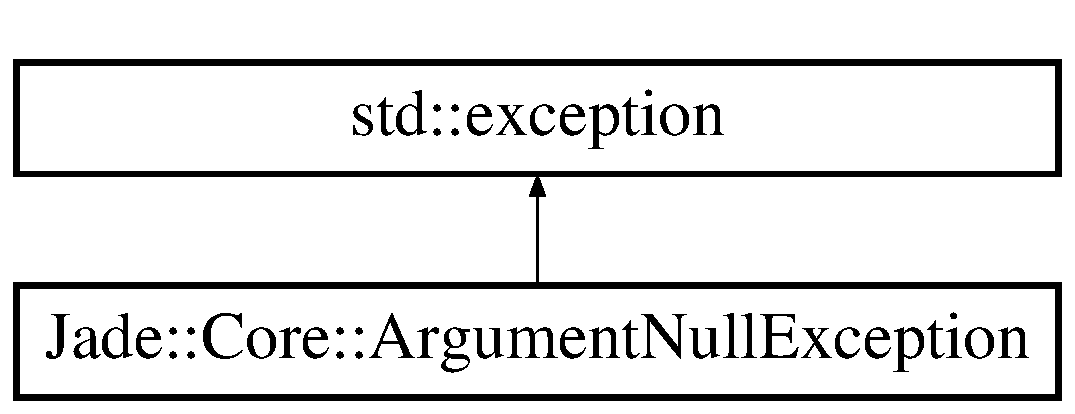
\includegraphics[height=2.000000cm]{class_jade_1_1_core_1_1_argument_null_exception}
\end{center}
\end{figure}
\subsection*{Public Member Functions}
\begin{DoxyCompactItemize}
\item 
\hypertarget{class_jade_1_1_core_1_1_argument_null_exception_a35c3013c192fe3c367e2c86a5dcb27b2}{}{\bfseries Argument\+Null\+Exception} (std\+::string parameter)\label{class_jade_1_1_core_1_1_argument_null_exception_a35c3013c192fe3c367e2c86a5dcb27b2}

\item 
\hypertarget{class_jade_1_1_core_1_1_argument_null_exception_a89ca4df20010e0ce6d64fde9c782af46}{}{\bfseries Argument\+Null\+Exception} (std\+::string parameter, std\+::string filename, int line)\label{class_jade_1_1_core_1_1_argument_null_exception_a89ca4df20010e0ce6d64fde9c782af46}

\item 
\hypertarget{class_jade_1_1_core_1_1_argument_null_exception_a41c747ac08349b4e0ab711a6e19d8553}{}const char $\ast$ {\bfseries what} () const  override  throw ()\label{class_jade_1_1_core_1_1_argument_null_exception_a41c747ac08349b4e0ab711a6e19d8553}

\item 
\hypertarget{class_jade_1_1_core_1_1_argument_null_exception_a750db6a7717709551e1a5542a1d39034}{}std\+::string {\bfseries Get\+Parameter} ()\label{class_jade_1_1_core_1_1_argument_null_exception_a750db6a7717709551e1a5542a1d39034}

\end{DoxyCompactItemize}


The documentation for this class was generated from the following file\+:\begin{DoxyCompactItemize}
\item 
C\+:/\+Users/\+Ben/\+Documents/\+Git\+Hub/\+Jade/\+Jade/\+Source/\+Core/\+Exception/Argument\+Null\+Exception.\+h\end{DoxyCompactItemize}

\hypertarget{class_jade_1_1_audio_1_1_audio_device}{}\section{Jade\+:\+:Audio\+:\+:Audio\+Device Class Reference}
\label{class_jade_1_1_audio_1_1_audio_device}\index{Jade\+::\+Audio\+::\+Audio\+Device@{Jade\+::\+Audio\+::\+Audio\+Device}}


The documentation for this class was generated from the following files\+:\begin{DoxyCompactItemize}
\item 
C\+:/\+Users/\+Ben/\+Documents/\+Git\+Hub/\+Jade/\+Jade/\+Source/\+Audio/Audio\+Device.\+h\item 
C\+:/\+Users/\+Ben/\+Documents/\+Git\+Hub/\+Jade/\+Jade/\+Source/\+Audio/Audio\+Device.\+cpp\end{DoxyCompactItemize}

\hypertarget{class_jade_1_1_graphics_1_1_blender}{}\section{Jade\+:\+:Graphics\+:\+:Blender Class Reference}
\label{class_jade_1_1_graphics_1_1_blender}\index{Jade\+::\+Graphics\+::\+Blender@{Jade\+::\+Graphics\+::\+Blender}}


The documentation for this class was generated from the following file\+:\begin{DoxyCompactItemize}
\item 
C\+:/\+Users/\+Ben/\+Documents/\+Git\+Hub/\+Jade/\+Jade/\+Source/\+Graphics/\+Blender/Blender.\+h\end{DoxyCompactItemize}

\hypertarget{class_jade_1_1_graphics_1_1_camera}{}\section{Jade\+:\+:Graphics\+:\+:Camera Class Reference}
\label{class_jade_1_1_graphics_1_1_camera}\index{Jade\+::\+Graphics\+::\+Camera@{Jade\+::\+Graphics\+::\+Camera}}
\subsection*{Public Member Functions}
\begin{DoxyCompactItemize}
\item 
\hypertarget{class_jade_1_1_graphics_1_1_camera_afde4506f9546df500a78a343877f8b24}{}{\bfseries Camera} (std\+::shared\+\_\+ptr$<$ \hyperlink{class_jade_1_1_graphics_1_1_device}{Device} $>$ device)\label{class_jade_1_1_graphics_1_1_camera_afde4506f9546df500a78a343877f8b24}

\item 
\hypertarget{class_jade_1_1_graphics_1_1_camera_a2d1efb3b8364a7c8fd463979cbacef64}{}void {\bfseries Look\+At} (\hyperlink{struct_jade_1_1_math_1_1_vector3}{Math\+::\+Vector3} position, \hyperlink{struct_jade_1_1_math_1_1_vector3}{Math\+::\+Vector3} target, \hyperlink{struct_jade_1_1_math_1_1_vector3}{Math\+::\+Vector3} direction)\label{class_jade_1_1_graphics_1_1_camera_a2d1efb3b8364a7c8fd463979cbacef64}

\end{DoxyCompactItemize}


The documentation for this class was generated from the following files\+:\begin{DoxyCompactItemize}
\item 
C\+:/\+Users/\+Ben/\+Documents/\+Git\+Hub/\+Jade/\+Jade/\+Source/\+Graphics/\+Camera/Camera.\+h\item 
C\+:/\+Users/\+Ben/\+Documents/\+Git\+Hub/\+Jade/\+Jade/\+Source/\+Graphics/\+Camera/Camera.\+cpp\end{DoxyCompactItemize}

\hypertarget{class_jade_1_1_graphics_1_1_canvas}{}\section{Jade\+:\+:Graphics\+:\+:Canvas Class Reference}
\label{class_jade_1_1_graphics_1_1_canvas}\index{Jade\+::\+Graphics\+::\+Canvas@{Jade\+::\+Graphics\+::\+Canvas}}


Represents a surface that can contain other sub-\/widgets such as buttons.  




{\ttfamily \#include $<$Canvas.\+h$>$}

Inheritance diagram for Jade\+:\+:Graphics\+:\+:Canvas\+:\begin{figure}[H]
\begin{center}
\leavevmode
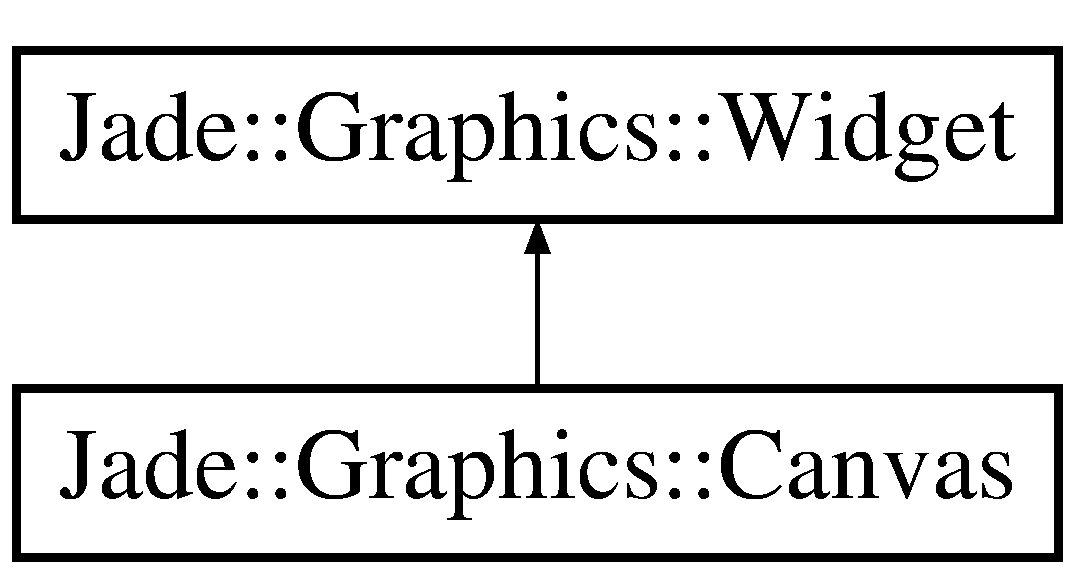
\includegraphics[height=2.000000cm]{class_jade_1_1_graphics_1_1_canvas}
\end{center}
\end{figure}
\subsection*{Public Member Functions}
\begin{DoxyCompactItemize}
\item 
\hypertarget{class_jade_1_1_graphics_1_1_canvas_a01d393cf06c44abfa47a90fd821dc8e6}{}\hyperlink{class_jade_1_1_math_1_1_point}{Math\+::\+Point} {\bfseries Get\+Position} () override\label{class_jade_1_1_graphics_1_1_canvas_a01d393cf06c44abfa47a90fd821dc8e6}

\item 
\hypertarget{class_jade_1_1_graphics_1_1_canvas_a49bd7c325e32d4b33186dd37c99eeaa0}{}void {\bfseries Set\+Position} (int x, int y) override\label{class_jade_1_1_graphics_1_1_canvas_a49bd7c325e32d4b33186dd37c99eeaa0}

\item 
\hypertarget{class_jade_1_1_graphics_1_1_canvas_a751e96de017443e39996dd0b7422b301}{}void {\bfseries Show} () override\label{class_jade_1_1_graphics_1_1_canvas_a751e96de017443e39996dd0b7422b301}

\item 
\hypertarget{class_jade_1_1_graphics_1_1_canvas_a64eb9015cdd78f996fcaa91bd55b37af}{}void {\bfseries Hide} () override\label{class_jade_1_1_graphics_1_1_canvas_a64eb9015cdd78f996fcaa91bd55b37af}

\item 
\hypertarget{class_jade_1_1_graphics_1_1_canvas_a56595e81b3df271caab041a7774d8645}{}void \hyperlink{class_jade_1_1_graphics_1_1_canvas_a56595e81b3df271caab041a7774d8645}{Draw} () override\label{class_jade_1_1_graphics_1_1_canvas_a56595e81b3df271caab041a7774d8645}

\begin{DoxyCompactList}\small\item\em Submits the widget information to the current device for rendering. \end{DoxyCompactList}\end{DoxyCompactItemize}


\subsection{Detailed Description}
Represents a surface that can contain other sub-\/widgets such as buttons. 

The documentation for this class was generated from the following files\+:\begin{DoxyCompactItemize}
\item 
C\+:/\+Users/\+Ben/\+Documents/\+Git\+Hub/\+Jade/\+Jade/\+Source/\+Graphics/\+Widget/Canvas.\+h\item 
C\+:/\+Users/\+Ben/\+Documents/\+Git\+Hub/\+Jade/\+Jade/\+Source/\+Graphics/\+Widget/Canvas.\+cpp\end{DoxyCompactItemize}

\hypertarget{struct_jade_1_1_math_1_1_color}{}\section{Jade\+:\+:Math\+:\+:Color Struct Reference}
\label{struct_jade_1_1_math_1_1_color}\index{Jade\+::\+Math\+::\+Color@{Jade\+::\+Math\+::\+Color}}
\subsection*{Public Member Functions}
\begin{DoxyCompactItemize}
\item 
\hypertarget{struct_jade_1_1_math_1_1_color_a4d6804a2c69e28e33ba7c0b6508d3a13}{}{\bfseries Color} (float red, float green, float blue, float alpha)\label{struct_jade_1_1_math_1_1_color_a4d6804a2c69e28e33ba7c0b6508d3a13}

\item 
\hypertarget{struct_jade_1_1_math_1_1_color_a0902c309c50466a4d091514d1ad185b9}{}float {\bfseries Get\+Red} () const \label{struct_jade_1_1_math_1_1_color_a0902c309c50466a4d091514d1ad185b9}

\item 
\hypertarget{struct_jade_1_1_math_1_1_color_a288ccfc00c16f2fd4f027932671c5d43}{}float {\bfseries Get\+Green} () const \label{struct_jade_1_1_math_1_1_color_a288ccfc00c16f2fd4f027932671c5d43}

\item 
\hypertarget{struct_jade_1_1_math_1_1_color_a06f9cd57dbaa7c4f63a29c0c4ac20002}{}float {\bfseries Get\+Blue} () const \label{struct_jade_1_1_math_1_1_color_a06f9cd57dbaa7c4f63a29c0c4ac20002}

\item 
\hypertarget{struct_jade_1_1_math_1_1_color_a088502e04369cba558d990447d25c56b}{}float {\bfseries Get\+Alpha} () const \label{struct_jade_1_1_math_1_1_color_a088502e04369cba558d990447d25c56b}

\end{DoxyCompactItemize}
\subsection*{Public Attributes}
\begin{DoxyCompactItemize}
\item 
\hypertarget{struct_jade_1_1_math_1_1_color_ab744343e6c623ca9759a6a2956a632d9}{}float {\bfseries red}\label{struct_jade_1_1_math_1_1_color_ab744343e6c623ca9759a6a2956a632d9}

\item 
\hypertarget{struct_jade_1_1_math_1_1_color_a5b4b945ae38e9c946c9e2ff22366d61f}{}float {\bfseries green}\label{struct_jade_1_1_math_1_1_color_a5b4b945ae38e9c946c9e2ff22366d61f}

\item 
\hypertarget{struct_jade_1_1_math_1_1_color_a09e622f39eff03be64ab70216a7a749c}{}float {\bfseries blue}\label{struct_jade_1_1_math_1_1_color_a09e622f39eff03be64ab70216a7a749c}

\item 
\hypertarget{struct_jade_1_1_math_1_1_color_a8abf15123eb28c1bfb3a2a2574d3c3b8}{}float {\bfseries alpha}\label{struct_jade_1_1_math_1_1_color_a8abf15123eb28c1bfb3a2a2574d3c3b8}

\end{DoxyCompactItemize}
\subsection*{Static Public Attributes}
\begin{DoxyCompactItemize}
\item 
\hypertarget{struct_jade_1_1_math_1_1_color_af00a42571acc758deb62c01289048b12}{}static const \hyperlink{struct_jade_1_1_math_1_1_color}{Color} {\bfseries Cornflower\+Blue}\label{struct_jade_1_1_math_1_1_color_af00a42571acc758deb62c01289048b12}

\item 
\hypertarget{struct_jade_1_1_math_1_1_color_a33b6ea31b79e67511383b98115b9de7b}{}static const \hyperlink{struct_jade_1_1_math_1_1_color}{Color} {\bfseries Red}\label{struct_jade_1_1_math_1_1_color_a33b6ea31b79e67511383b98115b9de7b}

\item 
\hypertarget{struct_jade_1_1_math_1_1_color_ab01e6c809ccdbee748e59c3be41548ec}{}static const \hyperlink{struct_jade_1_1_math_1_1_color}{Color} {\bfseries Green}\label{struct_jade_1_1_math_1_1_color_ab01e6c809ccdbee748e59c3be41548ec}

\item 
\hypertarget{struct_jade_1_1_math_1_1_color_a6c9a7df7d124049d5c81d6e426cd547b}{}static const \hyperlink{struct_jade_1_1_math_1_1_color}{Color} {\bfseries Blue}\label{struct_jade_1_1_math_1_1_color_a6c9a7df7d124049d5c81d6e426cd547b}

\item 
\hypertarget{struct_jade_1_1_math_1_1_color_ac198c2b6ba1a22793024bcd5b9585462}{}static const \hyperlink{struct_jade_1_1_math_1_1_color}{Color} {\bfseries Black}\label{struct_jade_1_1_math_1_1_color_ac198c2b6ba1a22793024bcd5b9585462}

\item 
\hypertarget{struct_jade_1_1_math_1_1_color_a1f530f70b7401db720b321de00f62a23}{}static const \hyperlink{struct_jade_1_1_math_1_1_color}{Color} {\bfseries Magenta}\label{struct_jade_1_1_math_1_1_color_a1f530f70b7401db720b321de00f62a23}

\item 
\hypertarget{struct_jade_1_1_math_1_1_color_a132d32c21e63bdd61f73093169756026}{}static const \hyperlink{struct_jade_1_1_math_1_1_color}{Color} {\bfseries Purple}\label{struct_jade_1_1_math_1_1_color_a132d32c21e63bdd61f73093169756026}

\item 
\hypertarget{struct_jade_1_1_math_1_1_color_ac554dd58a718baaad29898d740219a35}{}static const \hyperlink{struct_jade_1_1_math_1_1_color}{Color} {\bfseries White}\label{struct_jade_1_1_math_1_1_color_ac554dd58a718baaad29898d740219a35}

\item 
\hypertarget{struct_jade_1_1_math_1_1_color_a2c49358df2d84873f158ff184e0083bb}{}static const \hyperlink{struct_jade_1_1_math_1_1_color}{Color} {\bfseries Yellow}\label{struct_jade_1_1_math_1_1_color_a2c49358df2d84873f158ff184e0083bb}

\end{DoxyCompactItemize}


The documentation for this struct was generated from the following files\+:\begin{DoxyCompactItemize}
\item 
C\+:/\+Users/\+Ben/\+Documents/\+Git\+Hub/\+Jade/\+Jade/\+Source/\+Math/Color.\+h\item 
C\+:/\+Users/\+Ben/\+Documents/\+Git\+Hub/\+Jade/\+Jade/\+Source/\+Math/Color.\+cpp\end{DoxyCompactItemize}

\hypertarget{class_jade_1_1_system_1_1_configuration}{}\section{Jade\+:\+:System\+:\+:Configuration Class Reference}
\label{class_jade_1_1_system_1_1_configuration}\index{Jade\+::\+System\+::\+Configuration@{Jade\+::\+System\+::\+Configuration}}


The documentation for this class was generated from the following file\+:\begin{DoxyCompactItemize}
\item 
C\+:/\+Users/\+Ben/\+Documents/\+Git\+Hub/\+Jade/\+Jade/\+Source/\+System/Configuration.\+h\end{DoxyCompactItemize}

\hypertarget{class_jade_1_1_graphics_1_1_constant_buffer}{}\section{Jade\+:\+:Graphics\+:\+:Constant\+Buffer Class Reference}
\label{class_jade_1_1_graphics_1_1_constant_buffer}\index{Jade\+::\+Graphics\+::\+Constant\+Buffer@{Jade\+::\+Graphics\+::\+Constant\+Buffer}}
\subsection*{Public Member Functions}
\begin{DoxyCompactItemize}
\item 
\hypertarget{class_jade_1_1_graphics_1_1_constant_buffer_a411c8b44d703ce5a8f27305f9f2499da}{}{\bfseries Constant\+Buffer} (\hyperlink{class_jade_1_1_graphics_1_1_device}{Device} device, std\+::vector$<$ unsigned int $>$ indices, Usage usage)\label{class_jade_1_1_graphics_1_1_constant_buffer_a411c8b44d703ce5a8f27305f9f2499da}

\item 
\hypertarget{class_jade_1_1_graphics_1_1_constant_buffer_ad6543ed0c404a1a28ca498c20597e0dd}{}bool {\bfseries Bind} ()\label{class_jade_1_1_graphics_1_1_constant_buffer_ad6543ed0c404a1a28ca498c20597e0dd}

\item 
\hypertarget{class_jade_1_1_graphics_1_1_constant_buffer_aac9a4053f8e38a4157f7a1e98d37a292}{}bool {\bfseries Unbind} ()\label{class_jade_1_1_graphics_1_1_constant_buffer_aac9a4053f8e38a4157f7a1e98d37a292}

\end{DoxyCompactItemize}


The documentation for this class was generated from the following files\+:\begin{DoxyCompactItemize}
\item 
C\+:/\+Users/\+Ben/\+Documents/\+Git\+Hub/\+Jade/\+Jade/\+Source/\+Graphics/\+Buffer/Constant\+Buffer.\+h\item 
C\+:/\+Users/\+Ben/\+Documents/\+Git\+Hub/\+Jade/\+Jade/\+Source/\+Graphics/\+Buffer/Constant\+Buffer.\+cpp\end{DoxyCompactItemize}

\hypertarget{class_jade_1_1_graphics_1_1_device}{}\section{Jade\+:\+:Graphics\+:\+:Device Class Reference}
\label{class_jade_1_1_graphics_1_1_device}\index{Jade\+::\+Graphics\+::\+Device@{Jade\+::\+Graphics\+::\+Device}}
\subsection*{Public Member Functions}
\begin{DoxyCompactItemize}
\item 
\hypertarget{class_jade_1_1_graphics_1_1_device_ab6401c87d598e78d24406851054d31bf}{}{\bfseries Device} (std\+::shared\+\_\+ptr$<$ \hyperlink{class_jade_1_1_system_1_1_window}{System\+::\+Window} $>$ window, Graphics\+A\+P\+I api)\label{class_jade_1_1_graphics_1_1_device_ab6401c87d598e78d24406851054d31bf}

\item 
\hypertarget{class_jade_1_1_graphics_1_1_device_a44eed8c6de3bf0ea507204eaef8fe88e}{}{\bfseries Device} (std\+::shared\+\_\+ptr$<$ \hyperlink{struct_jade_1_1_system_1_1_i_window}{System\+::\+I\+Window} $>$ window, \hyperlink{struct_jade_1_1_graphics_1_1_specification}{Specification} specification)\label{class_jade_1_1_graphics_1_1_device_a44eed8c6de3bf0ea507204eaef8fe88e}

\item 
\hypertarget{class_jade_1_1_graphics_1_1_device_a95204aaf8684bd12c7a098a90ea0e3a3}{}{\bfseries Device} (std\+::shared\+\_\+ptr$<$ \hyperlink{class_jade_1_1_system_1_1_window}{System\+::\+Window} $>$ window, Graphics\+A\+P\+I api, \hyperlink{struct_jade_1_1_graphics_1_1_specification}{Specification} specification)\label{class_jade_1_1_graphics_1_1_device_a95204aaf8684bd12c7a098a90ea0e3a3}

\item 
\hypertarget{class_jade_1_1_graphics_1_1_device_acf66d5f61f5489f8081fea84b3752ac3}{}void {\bfseries Clear} (\hyperlink{struct_jade_1_1_math_1_1_color}{Math\+::\+Color} color) const \label{class_jade_1_1_graphics_1_1_device_acf66d5f61f5489f8081fea84b3752ac3}

\item 
\hypertarget{class_jade_1_1_graphics_1_1_device_a0808ac953233cdf240789f7e0dd678ce}{}void {\bfseries Hide\+Cursor} (bool toggle)\label{class_jade_1_1_graphics_1_1_device_a0808ac953233cdf240789f7e0dd678ce}

\item 
\hypertarget{class_jade_1_1_graphics_1_1_device_a037cd57e0e544caf0aaa793162cd23b3}{}void {\bfseries Present} () const \label{class_jade_1_1_graphics_1_1_device_a037cd57e0e544caf0aaa793162cd23b3}

\item 
\hypertarget{class_jade_1_1_graphics_1_1_device_a635de94382dbe1b6072d34bbc3222616}{}std\+::shared\+\_\+ptr$<$ \hyperlink{struct_jade_1_1_graphics_1_1_i_device}{I\+Device} $>$ {\bfseries Get\+I\+Device} () const \label{class_jade_1_1_graphics_1_1_device_a635de94382dbe1b6072d34bbc3222616}

\item 
\hypertarget{class_jade_1_1_graphics_1_1_device_add64b3329cc1039e842f4b9f67b7110d}{}Graphics\+A\+P\+I {\bfseries Get\+Graphics\+A\+P\+I} () const \label{class_jade_1_1_graphics_1_1_device_add64b3329cc1039e842f4b9f67b7110d}

\end{DoxyCompactItemize}


The documentation for this class was generated from the following files\+:\begin{DoxyCompactItemize}
\item 
C\+:/\+Users/\+Ben/\+Documents/\+Git\+Hub/\+Jade/\+Jade/\+Source/\+Graphics/\+Device/Device.\+h\item 
C\+:/\+Users/\+Ben/\+Documents/\+Git\+Hub/\+Jade/\+Jade/\+Source/\+Graphics/\+Device/Device.\+cpp\end{DoxyCompactItemize}

\hypertarget{class_jade_1_1_core_1_1_device_creation_exception}{}\section{Jade\+:\+:Core\+:\+:Device\+Creation\+Exception Class Reference}
\label{class_jade_1_1_core_1_1_device_creation_exception}\index{Jade\+::\+Core\+::\+Device\+Creation\+Exception@{Jade\+::\+Core\+::\+Device\+Creation\+Exception}}
Inheritance diagram for Jade\+:\+:Core\+:\+:Device\+Creation\+Exception\+:\begin{figure}[H]
\begin{center}
\leavevmode
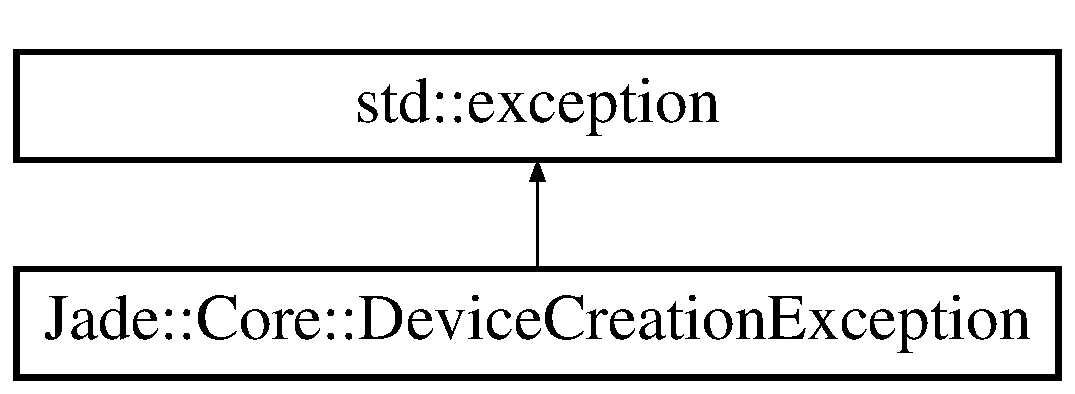
\includegraphics[height=2.000000cm]{class_jade_1_1_core_1_1_device_creation_exception}
\end{center}
\end{figure}
\subsection*{Public Member Functions}
\begin{DoxyCompactItemize}
\item 
\hypertarget{class_jade_1_1_core_1_1_device_creation_exception_a7cd301967a6f371f22028d7545997193}{}const char $\ast$ {\bfseries what} () const  override  throw ()\label{class_jade_1_1_core_1_1_device_creation_exception_a7cd301967a6f371f22028d7545997193}

\end{DoxyCompactItemize}


The documentation for this class was generated from the following file\+:\begin{DoxyCompactItemize}
\item 
C\+:/\+Users/\+Ben/\+Documents/\+Git\+Hub/\+Jade/\+Jade/\+Source/\+Core/\+Exception/Device\+Creation\+Exception.\+h\end{DoxyCompactItemize}

\hypertarget{class_jade_1_1_graphics_1_1_d_x_blender}{}\section{Jade\+:\+:Graphics\+:\+:D\+X\+Blender Class Reference}
\label{class_jade_1_1_graphics_1_1_d_x_blender}\index{Jade\+::\+Graphics\+::\+D\+X\+Blender@{Jade\+::\+Graphics\+::\+D\+X\+Blender}}
Inheritance diagram for Jade\+:\+:Graphics\+:\+:D\+X\+Blender\+:\begin{figure}[H]
\begin{center}
\leavevmode
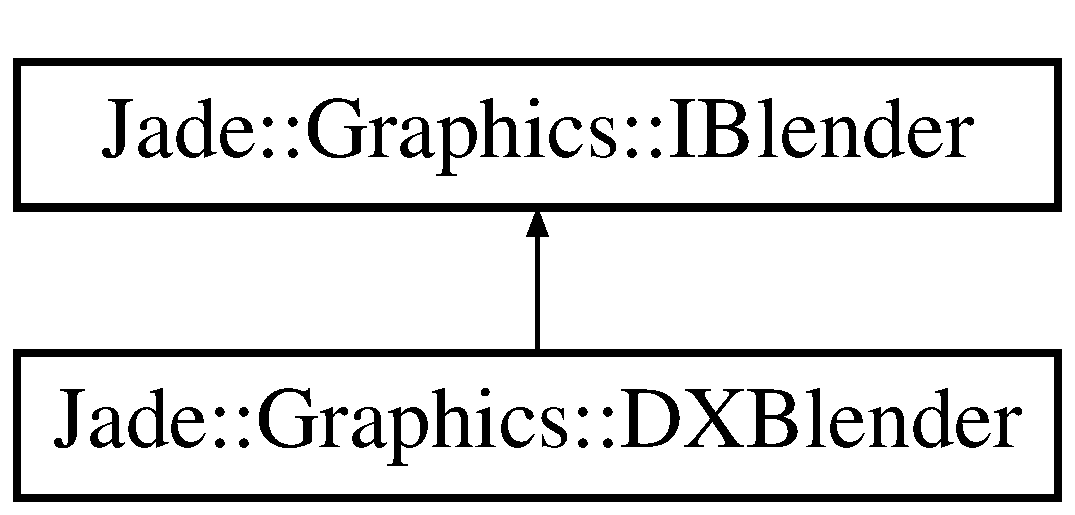
\includegraphics[height=2.000000cm]{class_jade_1_1_graphics_1_1_d_x_blender}
\end{center}
\end{figure}
\subsection*{Public Member Functions}
\begin{DoxyCompactItemize}
\item 
\hypertarget{class_jade_1_1_graphics_1_1_d_x_blender_a61676202a6e4ac9fe2120bb51f729f5e}{}{\bfseries D\+X\+Blender} (std\+::shared\+\_\+ptr$<$ D\+X\+Device $>$ device)\label{class_jade_1_1_graphics_1_1_d_x_blender_a61676202a6e4ac9fe2120bb51f729f5e}

\item 
\hypertarget{class_jade_1_1_graphics_1_1_d_x_blender_af73d473e115c375593a9985f6b310004}{}bool \hyperlink{class_jade_1_1_graphics_1_1_d_x_blender_af73d473e115c375593a9985f6b310004}{Set\+Blend\+State} (unsigned int mask) override\label{class_jade_1_1_graphics_1_1_d_x_blender_af73d473e115c375593a9985f6b310004}

\begin{DoxyCompactList}\small\item\em Sets the blend state for the specified mask value in hexadecimal. Example\+: 0xffffffff is the mask for enabling alpha blending. \end{DoxyCompactList}\end{DoxyCompactItemize}


The documentation for this class was generated from the following files\+:\begin{DoxyCompactItemize}
\item 
C\+:/\+Users/\+Ben/\+Documents/\+Git\+Hub/\+Jade/\+Jade/\+Source/\+Graphics/\+Blender/D\+X\+Blender.\+h\item 
C\+:/\+Users/\+Ben/\+Documents/\+Git\+Hub/\+Jade/\+Jade/\+Source/\+Graphics/\+Blender/D\+X\+Blender.\+cpp\end{DoxyCompactItemize}

\hypertarget{class_jade_1_1_system_1_1_file}{}\section{Jade\+:\+:System\+:\+:File Class Reference}
\label{class_jade_1_1_system_1_1_file}\index{Jade\+::\+System\+::\+File@{Jade\+::\+System\+::\+File}}
\subsection*{Public Member Functions}
\begin{DoxyCompactItemize}
\item 
\hypertarget{class_jade_1_1_system_1_1_file_a01eddcc244a22eaa378143b391d86204}{}{\bfseries File} (std\+::string filename)\label{class_jade_1_1_system_1_1_file_a01eddcc244a22eaa378143b391d86204}

\item 
\hypertarget{class_jade_1_1_system_1_1_file_a9c33a1c82a59eecd7b9f046a2e8f6e3c}{}std\+::string {\bfseries Read} ()\label{class_jade_1_1_system_1_1_file_a9c33a1c82a59eecd7b9f046a2e8f6e3c}

\item 
\hypertarget{class_jade_1_1_system_1_1_file_a899a6baf153ab70bc6d5f1bf000c3888}{}void {\bfseries Write} (std\+::string text)\label{class_jade_1_1_system_1_1_file_a899a6baf153ab70bc6d5f1bf000c3888}

\end{DoxyCompactItemize}


The documentation for this class was generated from the following file\+:\begin{DoxyCompactItemize}
\item 
C\+:/\+Users/\+Ben/\+Documents/\+Git\+Hub/\+Jade/\+Jade/\+Source/\+System/File.\+h\end{DoxyCompactItemize}

\hypertarget{class_jade_1_1_core_1_1_file_not_found_exception}{}\section{Jade\+:\+:Core\+:\+:File\+Not\+Found\+Exception Class Reference}
\label{class_jade_1_1_core_1_1_file_not_found_exception}\index{Jade\+::\+Core\+::\+File\+Not\+Found\+Exception@{Jade\+::\+Core\+::\+File\+Not\+Found\+Exception}}
Inheritance diagram for Jade\+:\+:Core\+:\+:File\+Not\+Found\+Exception\+:\begin{figure}[H]
\begin{center}
\leavevmode
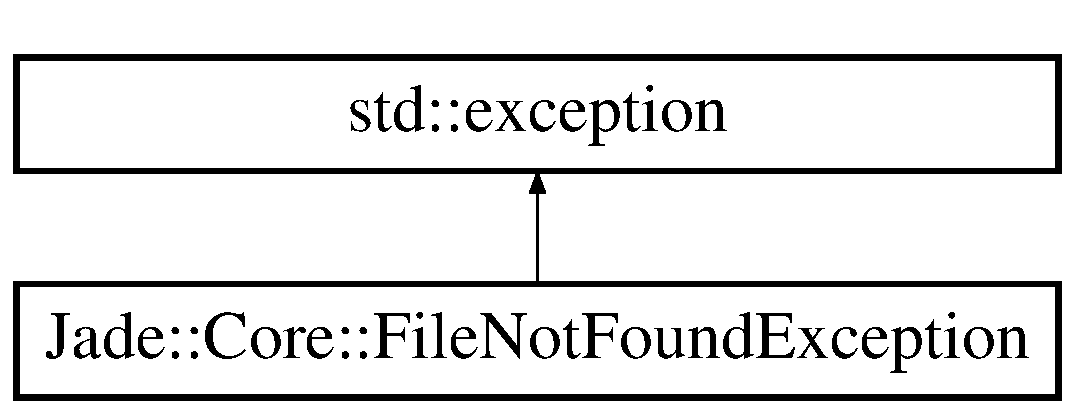
\includegraphics[height=2.000000cm]{class_jade_1_1_core_1_1_file_not_found_exception}
\end{center}
\end{figure}
\subsection*{Public Member Functions}
\begin{DoxyCompactItemize}
\item 
\hypertarget{class_jade_1_1_core_1_1_file_not_found_exception_ab236472ab38c52e761d895179205b847}{}\hyperlink{class_jade_1_1_core_1_1_file_not_found_exception_ab236472ab38c52e761d895179205b847}{File\+Not\+Found\+Exception} ()\label{class_jade_1_1_core_1_1_file_not_found_exception_ab236472ab38c52e761d895179205b847}

\begin{DoxyCompactList}\small\item\em Default error message. \end{DoxyCompactList}\item 
\hypertarget{class_jade_1_1_core_1_1_file_not_found_exception_aaf22ce3ffc2535d362755638a90a0196}{}\hyperlink{class_jade_1_1_core_1_1_file_not_found_exception_aaf22ce3ffc2535d362755638a90a0196}{File\+Not\+Found\+Exception} (std\+::string filename)\label{class_jade_1_1_core_1_1_file_not_found_exception_aaf22ce3ffc2535d362755638a90a0196}

\begin{DoxyCompactList}\small\item\em Error message with specified file name. \end{DoxyCompactList}\item 
\hypertarget{class_jade_1_1_core_1_1_file_not_found_exception_ad6478590ecd5056fac36a45f02a21b8f}{}const char $\ast$ {\bfseries what} () const  override  throw ()\label{class_jade_1_1_core_1_1_file_not_found_exception_ad6478590ecd5056fac36a45f02a21b8f}

\item 
\hypertarget{class_jade_1_1_core_1_1_file_not_found_exception_ae58c1710126d769e0cd895659cfa0af3}{}std\+::string {\bfseries Get\+Filename} ()\label{class_jade_1_1_core_1_1_file_not_found_exception_ae58c1710126d769e0cd895659cfa0af3}

\end{DoxyCompactItemize}


The documentation for this class was generated from the following file\+:\begin{DoxyCompactItemize}
\item 
C\+:/\+Users/\+Ben/\+Documents/\+Git\+Hub/\+Jade/\+Jade/\+Source/\+Core/\+Exception/File\+Not\+Found\+Exception.\+h\end{DoxyCompactItemize}

\hypertarget{class_jade_1_1_graphics_1_1_font}{}\section{Jade\+:\+:Graphics\+:\+:Font Class Reference}
\label{class_jade_1_1_graphics_1_1_font}\index{Jade\+::\+Graphics\+::\+Font@{Jade\+::\+Graphics\+::\+Font}}
\subsection*{Public Member Functions}
\begin{DoxyCompactItemize}
\item 
\hypertarget{class_jade_1_1_graphics_1_1_font_a74d474ba1237cad9f3a7127e84dcf13b}{}{\bfseries Font} (std\+::string filename)\label{class_jade_1_1_graphics_1_1_font_a74d474ba1237cad9f3a7127e84dcf13b}

\item 
\hypertarget{class_jade_1_1_graphics_1_1_font_a321193a4a9244e568bdaf344d65785c4}{}bool {\bfseries Load} ()\label{class_jade_1_1_graphics_1_1_font_a321193a4a9244e568bdaf344d65785c4}

\end{DoxyCompactItemize}


The documentation for this class was generated from the following files\+:\begin{DoxyCompactItemize}
\item 
C\+:/\+Users/\+Ben/\+Documents/\+Git\+Hub/\+Jade/\+Jade/\+Source/\+Graphics/\+Font/Font.\+h\item 
C\+:/\+Users/\+Ben/\+Documents/\+Git\+Hub/\+Jade/\+Jade/\+Source/\+Graphics/\+Font/Font.\+cpp\end{DoxyCompactItemize}

\hypertarget{class_jade_1_1_graphics_1_1_g_l_constant_buffer}{}\section{Jade\+:\+:Graphics\+:\+:G\+L\+Constant\+Buffer Class Reference}
\label{class_jade_1_1_graphics_1_1_g_l_constant_buffer}\index{Jade\+::\+Graphics\+::\+G\+L\+Constant\+Buffer@{Jade\+::\+Graphics\+::\+G\+L\+Constant\+Buffer}}
Inheritance diagram for Jade\+:\+:Graphics\+:\+:G\+L\+Constant\+Buffer\+:\begin{figure}[H]
\begin{center}
\leavevmode
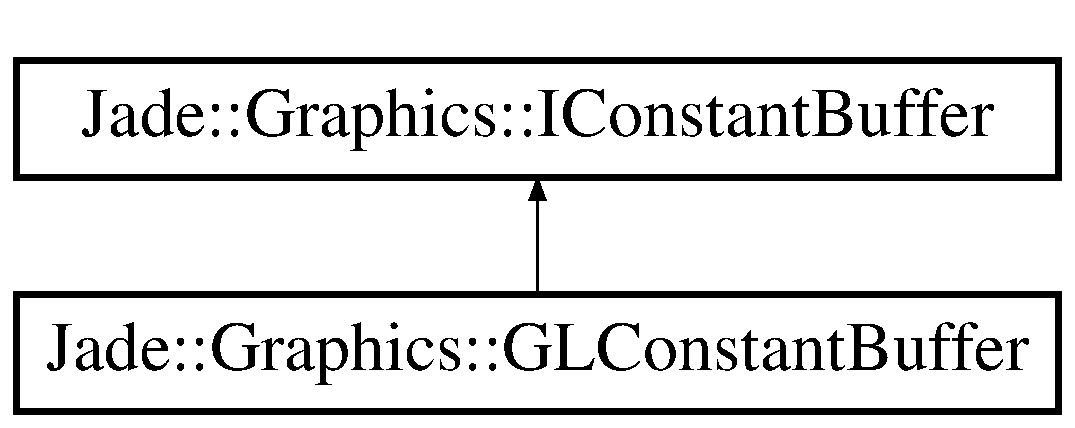
\includegraphics[height=2.000000cm]{class_jade_1_1_graphics_1_1_g_l_constant_buffer}
\end{center}
\end{figure}
\subsection*{Public Member Functions}
\begin{DoxyCompactItemize}
\item 
\hypertarget{class_jade_1_1_graphics_1_1_g_l_constant_buffer_a248bd27c22ec0bb6a0914d7c316eda43}{}bool {\bfseries Create\+View\+Matrix} () override\label{class_jade_1_1_graphics_1_1_g_l_constant_buffer_a248bd27c22ec0bb6a0914d7c316eda43}

\item 
\hypertarget{class_jade_1_1_graphics_1_1_g_l_constant_buffer_ac157f03e820e98b2b5487e55c3d8e57d}{}bool {\bfseries Create\+Projection\+Matrix} () override\label{class_jade_1_1_graphics_1_1_g_l_constant_buffer_ac157f03e820e98b2b5487e55c3d8e57d}

\item 
\hypertarget{class_jade_1_1_graphics_1_1_g_l_constant_buffer_a43f861a52e5112cc105db445bbe88600}{}bool {\bfseries Create\+World\+Matrix} () override\label{class_jade_1_1_graphics_1_1_g_l_constant_buffer_a43f861a52e5112cc105db445bbe88600}

\item 
\hypertarget{class_jade_1_1_graphics_1_1_g_l_constant_buffer_afdeb34f7b45223956976b31f764c5219}{}\hyperlink{struct_jade_1_1_math_1_1_matrix}{Math\+::\+Matrix} {\bfseries Get\+Projection\+Matrix} () override\label{class_jade_1_1_graphics_1_1_g_l_constant_buffer_afdeb34f7b45223956976b31f764c5219}

\item 
\hypertarget{class_jade_1_1_graphics_1_1_g_l_constant_buffer_a157d6fbeb07de79f61849487fe5ce083}{}\hyperlink{struct_jade_1_1_math_1_1_matrix}{Math\+::\+Matrix} {\bfseries Get\+View\+Matrix} () override\label{class_jade_1_1_graphics_1_1_g_l_constant_buffer_a157d6fbeb07de79f61849487fe5ce083}

\item 
\hypertarget{class_jade_1_1_graphics_1_1_g_l_constant_buffer_aefbb9b1883f7291bfa7bf6dbfc8afdca}{}\hyperlink{struct_jade_1_1_math_1_1_matrix}{Math\+::\+Matrix} {\bfseries Get\+World\+Matrix} () override\label{class_jade_1_1_graphics_1_1_g_l_constant_buffer_aefbb9b1883f7291bfa7bf6dbfc8afdca}

\item 
\hypertarget{class_jade_1_1_graphics_1_1_g_l_constant_buffer_a3c71669d4a5c5e322fa79136418bdd2d}{}void {\bfseries Set\+Projection\+Matrix} (\hyperlink{struct_jade_1_1_math_1_1_matrix}{Math\+::\+Matrix} matrix) override\label{class_jade_1_1_graphics_1_1_g_l_constant_buffer_a3c71669d4a5c5e322fa79136418bdd2d}

\item 
\hypertarget{class_jade_1_1_graphics_1_1_g_l_constant_buffer_a3f1b19332e2c9c722fefda645cc17bd7}{}void {\bfseries Set\+View\+Matrix} (\hyperlink{struct_jade_1_1_math_1_1_matrix}{Math\+::\+Matrix} matrix) override\label{class_jade_1_1_graphics_1_1_g_l_constant_buffer_a3f1b19332e2c9c722fefda645cc17bd7}

\item 
\hypertarget{class_jade_1_1_graphics_1_1_g_l_constant_buffer_abb593360ab818e716b23b034261e3809}{}void {\bfseries Set\+World\+Matrix} (\hyperlink{struct_jade_1_1_math_1_1_matrix}{Math\+::\+Matrix} matrix) override\label{class_jade_1_1_graphics_1_1_g_l_constant_buffer_abb593360ab818e716b23b034261e3809}

\item 
\hypertarget{class_jade_1_1_graphics_1_1_g_l_constant_buffer_a87e7d38c386290df46739be6dcf8410b}{}void {\bfseries Update} () override\label{class_jade_1_1_graphics_1_1_g_l_constant_buffer_a87e7d38c386290df46739be6dcf8410b}

\end{DoxyCompactItemize}


The documentation for this class was generated from the following files\+:\begin{DoxyCompactItemize}
\item 
C\+:/\+Users/\+Ben/\+Documents/\+Git\+Hub/\+Jade/\+Jade/\+Source/\+Graphics/\+Buffer/G\+L\+Constant\+Buffer.\+h\item 
C\+:/\+Users/\+Ben/\+Documents/\+Git\+Hub/\+Jade/\+Jade/\+Source/\+Graphics/\+Buffer/G\+L\+Constant\+Buffer.\+cpp\end{DoxyCompactItemize}

\hypertarget{class_jade_1_1_graphics_1_1_g_l_device}{}\section{Jade\+:\+:Graphics\+:\+:G\+L\+Device Class Reference}
\label{class_jade_1_1_graphics_1_1_g_l_device}\index{Jade\+::\+Graphics\+::\+G\+L\+Device@{Jade\+::\+Graphics\+::\+G\+L\+Device}}
Inheritance diagram for Jade\+:\+:Graphics\+:\+:G\+L\+Device\+:\begin{figure}[H]
\begin{center}
\leavevmode
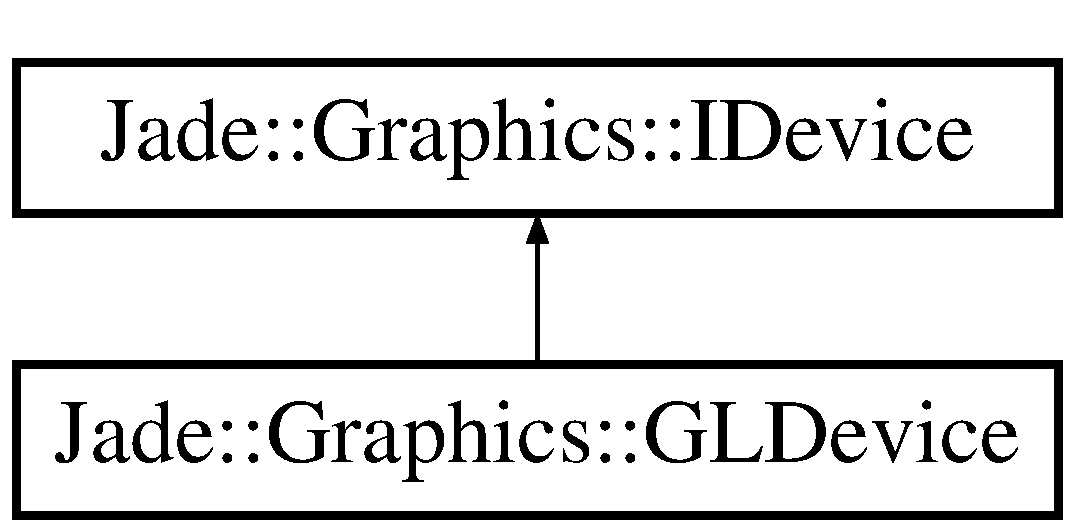
\includegraphics[height=2.000000cm]{class_jade_1_1_graphics_1_1_g_l_device}
\end{center}
\end{figure}
\subsection*{Public Member Functions}
\begin{DoxyCompactItemize}
\item 
\hypertarget{class_jade_1_1_graphics_1_1_g_l_device_af62110c6a84a1ef415f1ae17a2a78424}{}{\bfseries G\+L\+Device} (std\+::shared\+\_\+ptr$<$ \hyperlink{struct_jade_1_1_system_1_1_i_window}{System\+::\+I\+Window} $>$ window, \hyperlink{struct_jade_1_1_graphics_1_1_specification}{Specification} specification)\label{class_jade_1_1_graphics_1_1_g_l_device_af62110c6a84a1ef415f1ae17a2a78424}

\item 
\hypertarget{class_jade_1_1_graphics_1_1_g_l_device_a3787d704d6525c4bee4ed0596a83f739}{}void {\bfseries Clear} (\hyperlink{struct_jade_1_1_math_1_1_color}{Math\+::\+Color} color) override\label{class_jade_1_1_graphics_1_1_g_l_device_a3787d704d6525c4bee4ed0596a83f739}

\item 
\hypertarget{class_jade_1_1_graphics_1_1_g_l_device_a427a46a9d12fac4d130cf8dc656fb13d}{}void {\bfseries Present} () override\label{class_jade_1_1_graphics_1_1_g_l_device_a427a46a9d12fac4d130cf8dc656fb13d}

\item 
\hypertarget{class_jade_1_1_graphics_1_1_g_l_device_a17c8e8a20dc5689bc231fc3ead268be1}{}char $\ast$ {\bfseries Device\+Information} () override\label{class_jade_1_1_graphics_1_1_g_l_device_a17c8e8a20dc5689bc231fc3ead268be1}

\end{DoxyCompactItemize}


The documentation for this class was generated from the following files\+:\begin{DoxyCompactItemize}
\item 
C\+:/\+Users/\+Ben/\+Documents/\+Git\+Hub/\+Jade/\+Jade/\+Source/\+Graphics/\+Device/G\+L\+Device.\+h\item 
C\+:/\+Users/\+Ben/\+Documents/\+Git\+Hub/\+Jade/\+Jade/\+Source/\+Graphics/\+Device/G\+L\+Device.\+cpp\end{DoxyCompactItemize}

\hypertarget{class_jade_1_1_graphics_1_1_g_l_index_buffer}{}\section{Jade\+:\+:Graphics\+:\+:G\+L\+Index\+Buffer Class Reference}
\label{class_jade_1_1_graphics_1_1_g_l_index_buffer}\index{Jade\+::\+Graphics\+::\+G\+L\+Index\+Buffer@{Jade\+::\+Graphics\+::\+G\+L\+Index\+Buffer}}
Inheritance diagram for Jade\+:\+:Graphics\+:\+:G\+L\+Index\+Buffer\+:\begin{figure}[H]
\begin{center}
\leavevmode
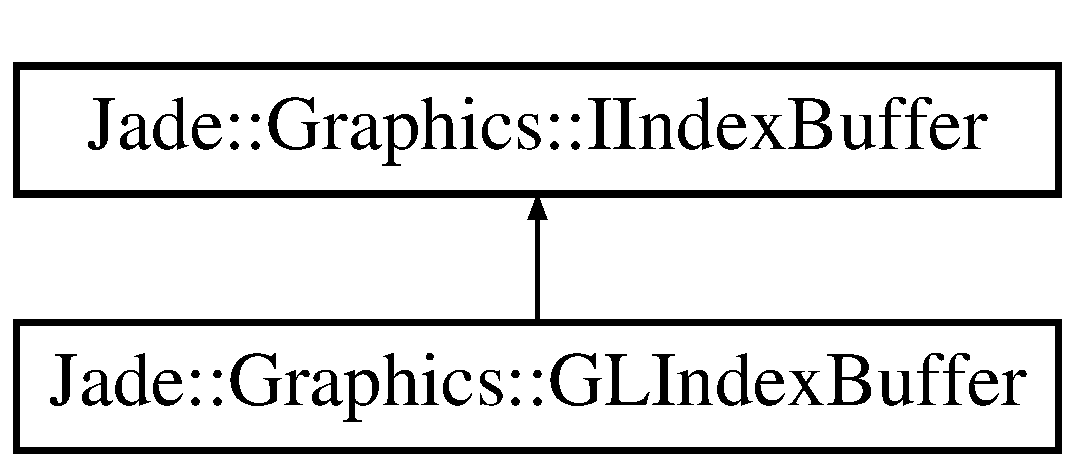
\includegraphics[height=2.000000cm]{class_jade_1_1_graphics_1_1_g_l_index_buffer}
\end{center}
\end{figure}
\subsection*{Public Member Functions}
\begin{DoxyCompactItemize}
\item 
\hypertarget{class_jade_1_1_graphics_1_1_g_l_index_buffer_a3e8a319cdbe847920db4c139de7b7cf4}{}{\bfseries G\+L\+Index\+Buffer} (std\+::vector$<$ unsigned int $>$ indices, Usage usage)\label{class_jade_1_1_graphics_1_1_g_l_index_buffer_a3e8a319cdbe847920db4c139de7b7cf4}

\item 
\hypertarget{class_jade_1_1_graphics_1_1_g_l_index_buffer_ae0408893f184bf928e981c82e2abdebf}{}bool {\bfseries Bind} () override\label{class_jade_1_1_graphics_1_1_g_l_index_buffer_ae0408893f184bf928e981c82e2abdebf}

\item 
\hypertarget{class_jade_1_1_graphics_1_1_g_l_index_buffer_ac41109d5752e2b18de21ef8827c04bc2}{}bool {\bfseries Unbind} () override\label{class_jade_1_1_graphics_1_1_g_l_index_buffer_ac41109d5752e2b18de21ef8827c04bc2}

\end{DoxyCompactItemize}


The documentation for this class was generated from the following files\+:\begin{DoxyCompactItemize}
\item 
C\+:/\+Users/\+Ben/\+Documents/\+Git\+Hub/\+Jade/\+Jade/\+Source/\+Graphics/\+Buffer/G\+L\+Index\+Buffer.\+h\item 
C\+:/\+Users/\+Ben/\+Documents/\+Git\+Hub/\+Jade/\+Jade/\+Source/\+Graphics/\+Buffer/G\+L\+Index\+Buffer.\+cpp\end{DoxyCompactItemize}

\hypertarget{class_jade_1_1_graphics_1_1_g_l_rasterizer}{}\section{Jade\+:\+:Graphics\+:\+:G\+L\+Rasterizer Class Reference}
\label{class_jade_1_1_graphics_1_1_g_l_rasterizer}\index{Jade\+::\+Graphics\+::\+G\+L\+Rasterizer@{Jade\+::\+Graphics\+::\+G\+L\+Rasterizer}}
Inheritance diagram for Jade\+:\+:Graphics\+:\+:G\+L\+Rasterizer\+:\begin{figure}[H]
\begin{center}
\leavevmode
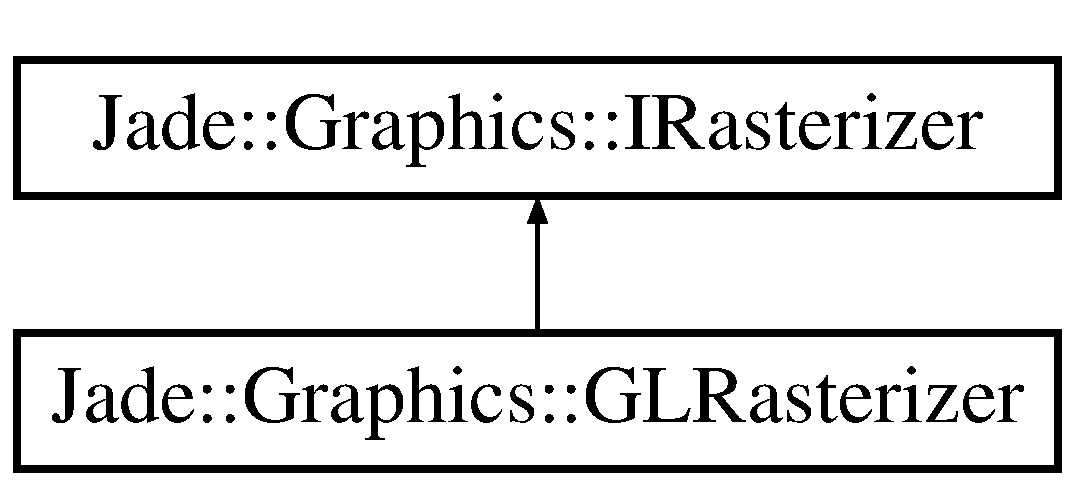
\includegraphics[height=2.000000cm]{class_jade_1_1_graphics_1_1_g_l_rasterizer}
\end{center}
\end{figure}
\subsection*{Public Member Functions}
\begin{DoxyCompactItemize}
\item 
\hypertarget{class_jade_1_1_graphics_1_1_g_l_rasterizer_a69b9b5adae0b32f4fb319b5d1557476e}{}bool {\bfseries Set\+Rasterizer\+State} (Cull\+Mode cull\+Mode, Fill\+Mode fill\+Mode, Wind\+Mode wind\+Mode) override\label{class_jade_1_1_graphics_1_1_g_l_rasterizer_a69b9b5adae0b32f4fb319b5d1557476e}

\item 
\hypertarget{class_jade_1_1_graphics_1_1_g_l_rasterizer_a8aff8db0e1955ca1de3d9bc01ab2e6d3}{}Cull\+Mode {\bfseries Get\+Cull\+Mode} () override\label{class_jade_1_1_graphics_1_1_g_l_rasterizer_a8aff8db0e1955ca1de3d9bc01ab2e6d3}

\item 
\hypertarget{class_jade_1_1_graphics_1_1_g_l_rasterizer_a4e9a2243d277a9222398c65446706a82}{}Fill\+Mode {\bfseries Get\+Fill\+Mode} () override\label{class_jade_1_1_graphics_1_1_g_l_rasterizer_a4e9a2243d277a9222398c65446706a82}

\item 
\hypertarget{class_jade_1_1_graphics_1_1_g_l_rasterizer_ab3b6b605967d04e3ee1b7cbcd8aad608}{}Wind\+Mode {\bfseries Get\+Wind\+Mode} () override\label{class_jade_1_1_graphics_1_1_g_l_rasterizer_ab3b6b605967d04e3ee1b7cbcd8aad608}

\end{DoxyCompactItemize}


The documentation for this class was generated from the following files\+:\begin{DoxyCompactItemize}
\item 
C\+:/\+Users/\+Ben/\+Documents/\+Git\+Hub/\+Jade/\+Jade/\+Source/\+Graphics/\+Rasterizer/G\+L\+Rasterizer.\+h\item 
C\+:/\+Users/\+Ben/\+Documents/\+Git\+Hub/\+Jade/\+Jade/\+Source/\+Graphics/\+Rasterizer/G\+L\+Rasterizer.\+cpp\end{DoxyCompactItemize}

\hypertarget{class_jade_1_1_graphics_1_1_g_l_shader}{}\section{Jade\+:\+:Graphics\+:\+:G\+L\+Shader Class Reference}
\label{class_jade_1_1_graphics_1_1_g_l_shader}\index{Jade\+::\+Graphics\+::\+G\+L\+Shader@{Jade\+::\+Graphics\+::\+G\+L\+Shader}}
Inheritance diagram for Jade\+:\+:Graphics\+:\+:G\+L\+Shader\+:\begin{figure}[H]
\begin{center}
\leavevmode
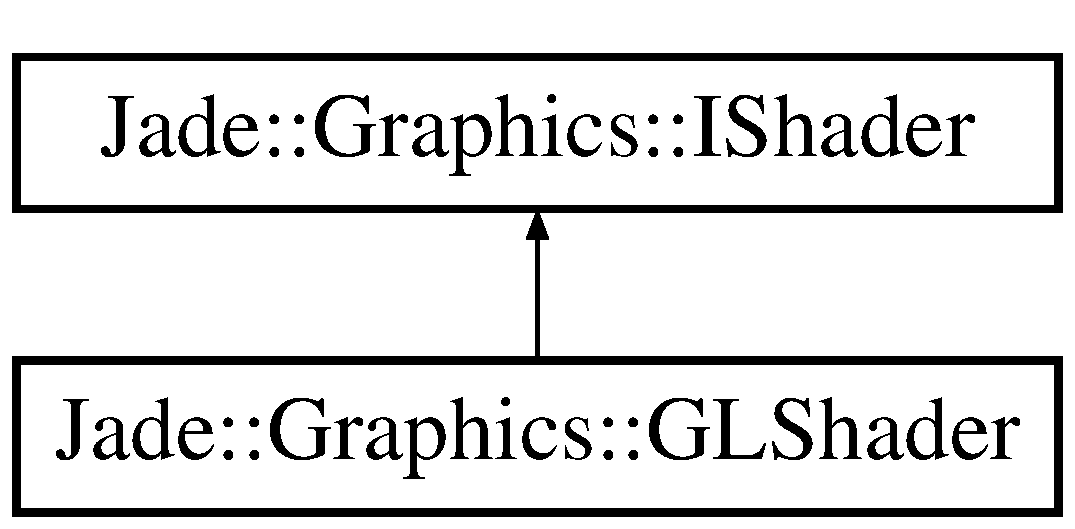
\includegraphics[height=2.000000cm]{class_jade_1_1_graphics_1_1_g_l_shader}
\end{center}
\end{figure}
\subsection*{Public Member Functions}
\begin{DoxyCompactItemize}
\item 
\hypertarget{class_jade_1_1_graphics_1_1_g_l_shader_a5428ee0d0ff44a8d18139ca7d9f86ce6}{}{\bfseries G\+L\+Shader} (std\+::string filename, Shader\+Type type)\label{class_jade_1_1_graphics_1_1_g_l_shader_a5428ee0d0ff44a8d18139ca7d9f86ce6}

\item 
\hypertarget{class_jade_1_1_graphics_1_1_g_l_shader_aa6d54ae78440642e692de0dad54f5940}{}bool {\bfseries Compile} () override\label{class_jade_1_1_graphics_1_1_g_l_shader_aa6d54ae78440642e692de0dad54f5940}

\end{DoxyCompactItemize}


The documentation for this class was generated from the following files\+:\begin{DoxyCompactItemize}
\item 
C\+:/\+Users/\+Ben/\+Documents/\+Git\+Hub/\+Jade/\+Jade/\+Source/\+Graphics/\+Shader/G\+L\+Shader.\+h\item 
C\+:/\+Users/\+Ben/\+Documents/\+Git\+Hub/\+Jade/\+Jade/\+Source/\+Graphics/\+Shader/G\+L\+Shader.\+cpp\end{DoxyCompactItemize}

\hypertarget{class_jade_1_1_graphics_1_1_g_l_vertex_buffer}{}\section{Jade\+:\+:Graphics\+:\+:G\+L\+Vertex\+Buffer Class Reference}
\label{class_jade_1_1_graphics_1_1_g_l_vertex_buffer}\index{Jade\+::\+Graphics\+::\+G\+L\+Vertex\+Buffer@{Jade\+::\+Graphics\+::\+G\+L\+Vertex\+Buffer}}
Inheritance diagram for Jade\+:\+:Graphics\+:\+:G\+L\+Vertex\+Buffer\+:\begin{figure}[H]
\begin{center}
\leavevmode
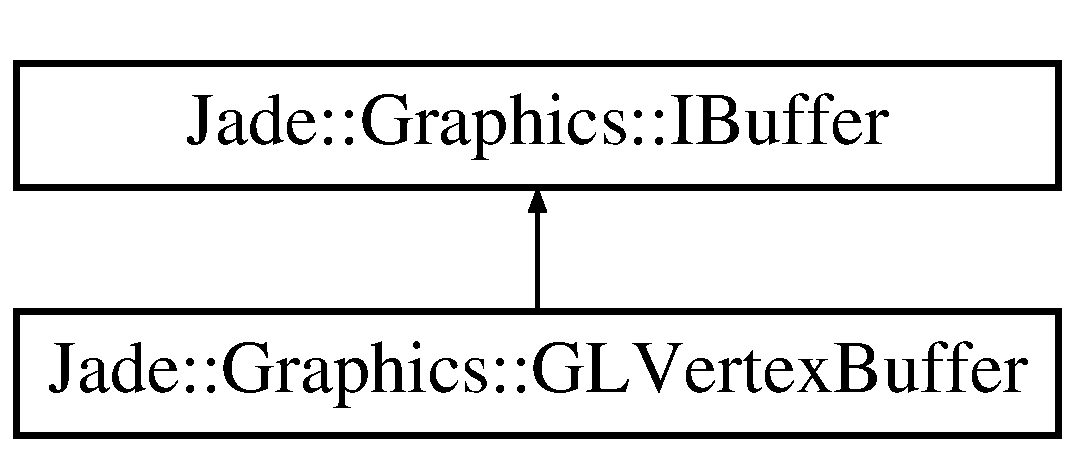
\includegraphics[height=2.000000cm]{class_jade_1_1_graphics_1_1_g_l_vertex_buffer}
\end{center}
\end{figure}
\subsection*{Public Member Functions}
\begin{DoxyCompactItemize}
\item 
\hypertarget{class_jade_1_1_graphics_1_1_g_l_vertex_buffer_af79d4779d5d4822bb0de36f03878b457}{}void {\bfseries Bind} () override\label{class_jade_1_1_graphics_1_1_g_l_vertex_buffer_af79d4779d5d4822bb0de36f03878b457}

\item 
\hypertarget{class_jade_1_1_graphics_1_1_g_l_vertex_buffer_acca109fdff3d6206217301eca1c1b9f2}{}bool {\bfseries Create} () override\label{class_jade_1_1_graphics_1_1_g_l_vertex_buffer_acca109fdff3d6206217301eca1c1b9f2}

\item 
\hypertarget{class_jade_1_1_graphics_1_1_g_l_vertex_buffer_a6d716c8443a36212e067b9b00b5206c8}{}std\+::vector$<$ \hyperlink{struct_jade_1_1_math_1_1_vertex}{Math\+::\+Vertex} $>$ {\bfseries Get\+Vertices} () override\label{class_jade_1_1_graphics_1_1_g_l_vertex_buffer_a6d716c8443a36212e067b9b00b5206c8}

\item 
\hypertarget{class_jade_1_1_graphics_1_1_g_l_vertex_buffer_a7b72fb56d2d741ebfdfe65e6a1df2963}{}void {\bfseries Set\+Vertices} (std\+::vector$<$ \hyperlink{struct_jade_1_1_math_1_1_vertex}{Math\+::\+Vertex} $>$ vertices) override\label{class_jade_1_1_graphics_1_1_g_l_vertex_buffer_a7b72fb56d2d741ebfdfe65e6a1df2963}

\item 
\hypertarget{class_jade_1_1_graphics_1_1_g_l_vertex_buffer_ae2b294bf5e590262e32a33e6223bf581}{}void {\bfseries Unbind} () override\label{class_jade_1_1_graphics_1_1_g_l_vertex_buffer_ae2b294bf5e590262e32a33e6223bf581}

\item 
\hypertarget{class_jade_1_1_graphics_1_1_g_l_vertex_buffer_ae2d6ee6503cd4a060ea8e03d2ecd3f00}{}void {\bfseries Update} () override\label{class_jade_1_1_graphics_1_1_g_l_vertex_buffer_ae2d6ee6503cd4a060ea8e03d2ecd3f00}

\end{DoxyCompactItemize}


The documentation for this class was generated from the following files\+:\begin{DoxyCompactItemize}
\item 
C\+:/\+Users/\+Ben/\+Documents/\+Git\+Hub/\+Jade/\+Jade/\+Source/\+Graphics/\+Buffer/G\+L\+Vertex\+Buffer.\+h\item 
C\+:/\+Users/\+Ben/\+Documents/\+Git\+Hub/\+Jade/\+Jade/\+Source/\+Graphics/\+Buffer/G\+L\+Vertex\+Buffer.\+cpp\end{DoxyCompactItemize}

\hypertarget{struct_jade_1_1_graphics_1_1_glyph}{}\section{Jade\+:\+:Graphics\+:\+:Glyph Struct Reference}
\label{struct_jade_1_1_graphics_1_1_glyph}\index{Jade\+::\+Graphics\+::\+Glyph@{Jade\+::\+Graphics\+::\+Glyph}}
\subsection*{Public Attributes}
\begin{DoxyCompactItemize}
\item 
\hypertarget{struct_jade_1_1_graphics_1_1_glyph_af138396cfdec108c776fa599a14ba1e4}{}char {\bfseries character}\label{struct_jade_1_1_graphics_1_1_glyph_af138396cfdec108c776fa599a14ba1e4}

\item 
\hypertarget{struct_jade_1_1_graphics_1_1_glyph_a9b2276dc59b681731d0514a518fc672b}{}int {\bfseries width}\label{struct_jade_1_1_graphics_1_1_glyph_a9b2276dc59b681731d0514a518fc672b}

\item 
\hypertarget{struct_jade_1_1_graphics_1_1_glyph_a184d5d7e52652dedc12e22daf1aba744}{}int {\bfseries height}\label{struct_jade_1_1_graphics_1_1_glyph_a184d5d7e52652dedc12e22daf1aba744}

\item 
\hypertarget{struct_jade_1_1_graphics_1_1_glyph_a7622231925e54848d31ebbf3285bec61}{}int {\bfseries x\+Offset}\label{struct_jade_1_1_graphics_1_1_glyph_a7622231925e54848d31ebbf3285bec61}

\item 
\hypertarget{struct_jade_1_1_graphics_1_1_glyph_a5f16756ac11d5dfd697ad877c208dd96}{}int {\bfseries y\+Offset}\label{struct_jade_1_1_graphics_1_1_glyph_a5f16756ac11d5dfd697ad877c208dd96}

\item 
\hypertarget{struct_jade_1_1_graphics_1_1_glyph_a081f1bbf645e08811dea4bcf50a60c59}{}int {\bfseries advance}\label{struct_jade_1_1_graphics_1_1_glyph_a081f1bbf645e08811dea4bcf50a60c59}

\item 
\hypertarget{struct_jade_1_1_graphics_1_1_glyph_a83aa50d0eba411475adebb795d731b2e}{}float {\bfseries u}\label{struct_jade_1_1_graphics_1_1_glyph_a83aa50d0eba411475adebb795d731b2e}

\item 
\hypertarget{struct_jade_1_1_graphics_1_1_glyph_a3b15cafd58a0dd8b9aff8261e69e2946}{}float {\bfseries v}\label{struct_jade_1_1_graphics_1_1_glyph_a3b15cafd58a0dd8b9aff8261e69e2946}

\end{DoxyCompactItemize}


The documentation for this struct was generated from the following file\+:\begin{DoxyCompactItemize}
\item 
C\+:/\+Users/\+Ben/\+Documents/\+Git\+Hub/\+Jade/\+Jade/\+Source/\+Graphics/\+Font/Glyph.\+h\end{DoxyCompactItemize}

\hypertarget{class_jade_1_1_math_1_1_helper}{}\section{Jade\+:\+:Math\+:\+:Helper Class Reference}
\label{class_jade_1_1_math_1_1_helper}\index{Jade\+::\+Math\+::\+Helper@{Jade\+::\+Math\+::\+Helper}}
\subsection*{Static Public Member Functions}
\begin{DoxyCompactItemize}
\item 
\hypertarget{class_jade_1_1_math_1_1_helper_a659eb850509ac325edf5f9f43745cffd}{}static float {\bfseries Fast\+Inv\+Sqrt} (float x)\label{class_jade_1_1_math_1_1_helper_a659eb850509ac325edf5f9f43745cffd}

\item 
\hypertarget{class_jade_1_1_math_1_1_helper_a81040c88535f64bc41143ad3be058c74}{}static float {\bfseries Wrap\+Angle} (float angle)\label{class_jade_1_1_math_1_1_helper_a81040c88535f64bc41143ad3be058c74}

\end{DoxyCompactItemize}


The documentation for this class was generated from the following files\+:\begin{DoxyCompactItemize}
\item 
C\+:/\+Users/\+Ben/\+Documents/\+Git\+Hub/\+Jade/\+Jade/\+Source/\+Math/Helper.\+h\item 
C\+:/\+Users/\+Ben/\+Documents/\+Git\+Hub/\+Jade/\+Jade/\+Source/\+Math/Helper.\+cpp\end{DoxyCompactItemize}

\hypertarget{struct_jade_1_1_graphics_1_1_i_blender}{}\section{Jade\+:\+:Graphics\+:\+:I\+Blender Struct Reference}
\label{struct_jade_1_1_graphics_1_1_i_blender}\index{Jade\+::\+Graphics\+::\+I\+Blender@{Jade\+::\+Graphics\+::\+I\+Blender}}
Inheritance diagram for Jade\+:\+:Graphics\+:\+:I\+Blender\+:\begin{figure}[H]
\begin{center}
\leavevmode
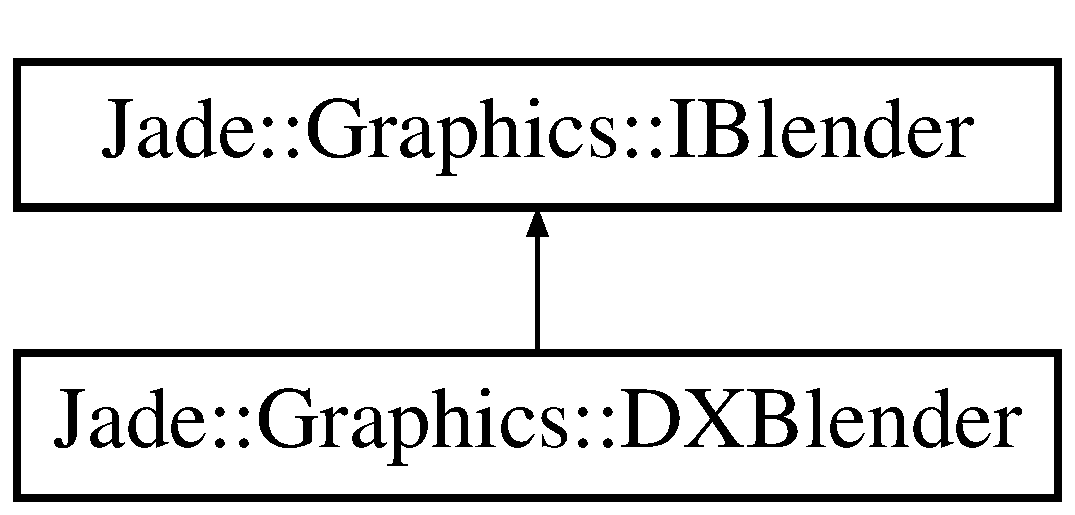
\includegraphics[height=2.000000cm]{struct_jade_1_1_graphics_1_1_i_blender}
\end{center}
\end{figure}
\subsection*{Public Member Functions}
\begin{DoxyCompactItemize}
\item 
\hypertarget{struct_jade_1_1_graphics_1_1_i_blender_a9319325ed247f55038d21afc73b11cca}{}virtual bool {\bfseries Set\+Blend\+State} (unsigned int mask)=0\label{struct_jade_1_1_graphics_1_1_i_blender_a9319325ed247f55038d21afc73b11cca}

\end{DoxyCompactItemize}


The documentation for this struct was generated from the following file\+:\begin{DoxyCompactItemize}
\item 
C\+:/\+Users/\+Ben/\+Documents/\+Git\+Hub/\+Jade/\+Jade/\+Source/\+Graphics/\+Blender/I\+Blender.\+h\end{DoxyCompactItemize}

\hypertarget{struct_jade_1_1_graphics_1_1_i_constant_buffer}{}\section{Jade\+:\+:Graphics\+:\+:I\+Constant\+Buffer Struct Reference}
\label{struct_jade_1_1_graphics_1_1_i_constant_buffer}\index{Jade\+::\+Graphics\+::\+I\+Constant\+Buffer@{Jade\+::\+Graphics\+::\+I\+Constant\+Buffer}}
Inheritance diagram for Jade\+:\+:Graphics\+:\+:I\+Constant\+Buffer\+:\begin{figure}[H]
\begin{center}
\leavevmode
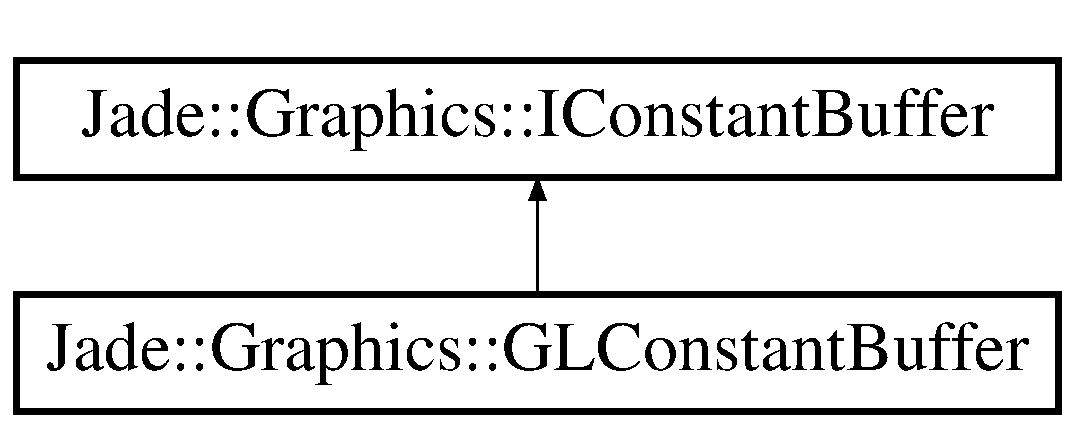
\includegraphics[height=2.000000cm]{struct_jade_1_1_graphics_1_1_i_constant_buffer}
\end{center}
\end{figure}
\subsection*{Public Member Functions}
\begin{DoxyCompactItemize}
\item 
\hypertarget{struct_jade_1_1_graphics_1_1_i_constant_buffer_a431d36b403634475b18ff34d8160f417}{}virtual bool {\bfseries Create\+Projection\+Matrix} ()=0\label{struct_jade_1_1_graphics_1_1_i_constant_buffer_a431d36b403634475b18ff34d8160f417}

\item 
\hypertarget{struct_jade_1_1_graphics_1_1_i_constant_buffer_af2097d8df9756fe2dbcfa5e73a7b623d}{}virtual bool {\bfseries Create\+View\+Matrix} ()=0\label{struct_jade_1_1_graphics_1_1_i_constant_buffer_af2097d8df9756fe2dbcfa5e73a7b623d}

\item 
\hypertarget{struct_jade_1_1_graphics_1_1_i_constant_buffer_adb6345c5c452cae4bc17e53e04babb81}{}virtual bool {\bfseries Create\+World\+Matrix} ()=0\label{struct_jade_1_1_graphics_1_1_i_constant_buffer_adb6345c5c452cae4bc17e53e04babb81}

\item 
\hypertarget{struct_jade_1_1_graphics_1_1_i_constant_buffer_aa7eaa1c2225706c56ffe845aac858021}{}virtual \hyperlink{struct_jade_1_1_math_1_1_matrix}{Math\+::\+Matrix} {\bfseries Get\+Projection\+Matrix} ()=0\label{struct_jade_1_1_graphics_1_1_i_constant_buffer_aa7eaa1c2225706c56ffe845aac858021}

\item 
\hypertarget{struct_jade_1_1_graphics_1_1_i_constant_buffer_a916256650c5abc057f6718573a16e24c}{}virtual \hyperlink{struct_jade_1_1_math_1_1_matrix}{Math\+::\+Matrix} {\bfseries Get\+View\+Matrix} ()=0\label{struct_jade_1_1_graphics_1_1_i_constant_buffer_a916256650c5abc057f6718573a16e24c}

\item 
\hypertarget{struct_jade_1_1_graphics_1_1_i_constant_buffer_af1b121fd9ced9db28491a9260de012ce}{}virtual \hyperlink{struct_jade_1_1_math_1_1_matrix}{Math\+::\+Matrix} {\bfseries Get\+World\+Matrix} ()=0\label{struct_jade_1_1_graphics_1_1_i_constant_buffer_af1b121fd9ced9db28491a9260de012ce}

\item 
\hypertarget{struct_jade_1_1_graphics_1_1_i_constant_buffer_afd72c1014e5cc1f90d76b4cdf0233a6a}{}virtual void {\bfseries Set\+Projection\+Matrix} (\hyperlink{struct_jade_1_1_math_1_1_matrix}{Math\+::\+Matrix} matrix)=0\label{struct_jade_1_1_graphics_1_1_i_constant_buffer_afd72c1014e5cc1f90d76b4cdf0233a6a}

\item 
\hypertarget{struct_jade_1_1_graphics_1_1_i_constant_buffer_a259c407613711ee0fd5158f51f492556}{}virtual void {\bfseries Set\+View\+Matrix} (\hyperlink{struct_jade_1_1_math_1_1_matrix}{Math\+::\+Matrix} matrix)=0\label{struct_jade_1_1_graphics_1_1_i_constant_buffer_a259c407613711ee0fd5158f51f492556}

\item 
\hypertarget{struct_jade_1_1_graphics_1_1_i_constant_buffer_a4d7aca82baa2d5a549f87bac337b01db}{}virtual void {\bfseries Set\+World\+Matrix} (\hyperlink{struct_jade_1_1_math_1_1_matrix}{Math\+::\+Matrix} matrix)=0\label{struct_jade_1_1_graphics_1_1_i_constant_buffer_a4d7aca82baa2d5a549f87bac337b01db}

\item 
\hypertarget{struct_jade_1_1_graphics_1_1_i_constant_buffer_ace4b76bd5cd1524562c6ea4abd1a8579}{}virtual void {\bfseries Update} ()=0\label{struct_jade_1_1_graphics_1_1_i_constant_buffer_ace4b76bd5cd1524562c6ea4abd1a8579}

\end{DoxyCompactItemize}


The documentation for this struct was generated from the following file\+:\begin{DoxyCompactItemize}
\item 
C\+:/\+Users/\+Ben/\+Documents/\+Git\+Hub/\+Jade/\+Jade/\+Source/\+Graphics/\+Buffer/I\+Constant\+Buffer.\+h\end{DoxyCompactItemize}

\hypertarget{struct_jade_1_1_graphics_1_1_i_device}{}\section{Jade\+:\+:Graphics\+:\+:I\+Device Struct Reference}
\label{struct_jade_1_1_graphics_1_1_i_device}\index{Jade\+::\+Graphics\+::\+I\+Device@{Jade\+::\+Graphics\+::\+I\+Device}}
Inheritance diagram for Jade\+:\+:Graphics\+:\+:I\+Device\+:\begin{figure}[H]
\begin{center}
\leavevmode
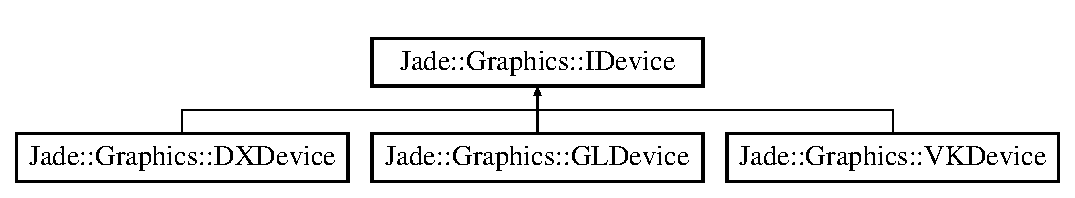
\includegraphics[height=2.000000cm]{struct_jade_1_1_graphics_1_1_i_device}
\end{center}
\end{figure}
\subsection*{Public Member Functions}
\begin{DoxyCompactItemize}
\item 
\hypertarget{struct_jade_1_1_graphics_1_1_i_device_ab898bda6f3b99c18b4c4dd939ec3b138}{}virtual void {\bfseries Clear} (\hyperlink{struct_jade_1_1_math_1_1_color}{Math\+::\+Color} color)=0\label{struct_jade_1_1_graphics_1_1_i_device_ab898bda6f3b99c18b4c4dd939ec3b138}

\item 
\hypertarget{struct_jade_1_1_graphics_1_1_i_device_a67c38c0ca3031f1e959cf569ba25fec3}{}virtual void {\bfseries Present} ()=0\label{struct_jade_1_1_graphics_1_1_i_device_a67c38c0ca3031f1e959cf569ba25fec3}

\item 
\hypertarget{struct_jade_1_1_graphics_1_1_i_device_a4ef23421fe5c8bcd09731a1d38eda78f}{}virtual char $\ast$ {\bfseries Device\+Information} ()=0\label{struct_jade_1_1_graphics_1_1_i_device_a4ef23421fe5c8bcd09731a1d38eda78f}

\end{DoxyCompactItemize}


The documentation for this struct was generated from the following file\+:\begin{DoxyCompactItemize}
\item 
C\+:/\+Users/\+Ben/\+Documents/\+Git\+Hub/\+Jade/\+Jade/\+Source/\+Graphics/\+Device/I\+Device.\+h\end{DoxyCompactItemize}

\hypertarget{struct_jade_1_1_graphics_1_1_i_index_buffer}{}\section{Jade\+:\+:Graphics\+:\+:I\+Index\+Buffer Struct Reference}
\label{struct_jade_1_1_graphics_1_1_i_index_buffer}\index{Jade\+::\+Graphics\+::\+I\+Index\+Buffer@{Jade\+::\+Graphics\+::\+I\+Index\+Buffer}}
Inheritance diagram for Jade\+:\+:Graphics\+:\+:I\+Index\+Buffer\+:\begin{figure}[H]
\begin{center}
\leavevmode
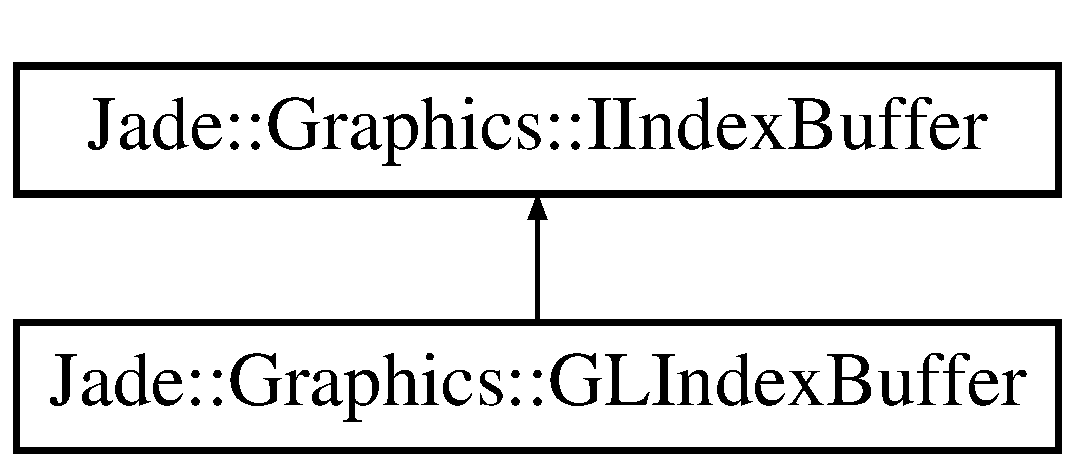
\includegraphics[height=2.000000cm]{struct_jade_1_1_graphics_1_1_i_index_buffer}
\end{center}
\end{figure}
\subsection*{Public Member Functions}
\begin{DoxyCompactItemize}
\item 
\hypertarget{struct_jade_1_1_graphics_1_1_i_index_buffer_a3be2d4a86df4b74a12f9a9143beb7719}{}virtual void {\bfseries Bind} ()=0\label{struct_jade_1_1_graphics_1_1_i_index_buffer_a3be2d4a86df4b74a12f9a9143beb7719}

\item 
\hypertarget{struct_jade_1_1_graphics_1_1_i_index_buffer_ae3e3e519a3f71f92b25f45d84a40e2d0}{}virtual bool {\bfseries Create} ()=0\label{struct_jade_1_1_graphics_1_1_i_index_buffer_ae3e3e519a3f71f92b25f45d84a40e2d0}

\item 
\hypertarget{struct_jade_1_1_graphics_1_1_i_index_buffer_a15aec0fcb1b301c43ca181631c966fdd}{}virtual std\+::vector$<$ unsigned short $>$ {\bfseries Get\+Indices} ()=0\label{struct_jade_1_1_graphics_1_1_i_index_buffer_a15aec0fcb1b301c43ca181631c966fdd}

\item 
\hypertarget{struct_jade_1_1_graphics_1_1_i_index_buffer_a099e502c707522af54532e365626c4d3}{}virtual void {\bfseries Set\+Indices} (std\+::vector$<$ unsigned short $>$ indices)=0\label{struct_jade_1_1_graphics_1_1_i_index_buffer_a099e502c707522af54532e365626c4d3}

\item 
\hypertarget{struct_jade_1_1_graphics_1_1_i_index_buffer_a1bd3c981a87bf63434d5a858def2c63a}{}virtual void {\bfseries Unbind} ()=0\label{struct_jade_1_1_graphics_1_1_i_index_buffer_a1bd3c981a87bf63434d5a858def2c63a}

\item 
\hypertarget{struct_jade_1_1_graphics_1_1_i_index_buffer_a15a6b13ff2f5c63c6c83c5d142bc26ac}{}virtual void {\bfseries Update} ()=0\label{struct_jade_1_1_graphics_1_1_i_index_buffer_a15a6b13ff2f5c63c6c83c5d142bc26ac}

\end{DoxyCompactItemize}


The documentation for this struct was generated from the following file\+:\begin{DoxyCompactItemize}
\item 
C\+:/\+Users/\+Ben/\+Documents/\+Git\+Hub/\+Jade/\+Jade/\+Source/\+Graphics/\+Buffer/I\+Index\+Buffer.\+h\end{DoxyCompactItemize}

\hypertarget{class_jade_1_1_graphics_1_1_index_buffer}{}\section{Jade\+:\+:Graphics\+:\+:Index\+Buffer Class Reference}
\label{class_jade_1_1_graphics_1_1_index_buffer}\index{Jade\+::\+Graphics\+::\+Index\+Buffer@{Jade\+::\+Graphics\+::\+Index\+Buffer}}
\subsection*{Public Member Functions}
\begin{DoxyCompactItemize}
\item 
\hypertarget{class_jade_1_1_graphics_1_1_index_buffer_a5ee1d8d465fb994fd7ddbe24e3f1ac3e}{}{\bfseries Index\+Buffer} (std\+::shared\+\_\+ptr$<$ \hyperlink{class_jade_1_1_graphics_1_1_device}{Device} $>$ device, std\+::vector$<$ unsigned int $>$ indices, Usage usage)\label{class_jade_1_1_graphics_1_1_index_buffer_a5ee1d8d465fb994fd7ddbe24e3f1ac3e}

\item 
\hypertarget{class_jade_1_1_graphics_1_1_index_buffer_a0020156990c8c19bc17ebe6c5340866c}{}bool {\bfseries Bind} ()\label{class_jade_1_1_graphics_1_1_index_buffer_a0020156990c8c19bc17ebe6c5340866c}

\item 
\hypertarget{class_jade_1_1_graphics_1_1_index_buffer_a0d8c31d5335824573cf287a3e5ea8272}{}bool {\bfseries Unbind} ()\label{class_jade_1_1_graphics_1_1_index_buffer_a0d8c31d5335824573cf287a3e5ea8272}

\end{DoxyCompactItemize}


The documentation for this class was generated from the following files\+:\begin{DoxyCompactItemize}
\item 
C\+:/\+Users/\+Ben/\+Documents/\+Git\+Hub/\+Jade/\+Jade/\+Source/\+Graphics/\+Buffer/Index\+Buffer.\+h\item 
C\+:/\+Users/\+Ben/\+Documents/\+Git\+Hub/\+Jade/\+Jade/\+Source/\+Graphics/\+Buffer/Index\+Buffer.\+cpp\end{DoxyCompactItemize}

\hypertarget{class_jade_1_1_core_1_1_initialization_exception}{}\section{Jade\+:\+:Core\+:\+:Initialization\+Exception Class Reference}
\label{class_jade_1_1_core_1_1_initialization_exception}\index{Jade\+::\+Core\+::\+Initialization\+Exception@{Jade\+::\+Core\+::\+Initialization\+Exception}}
Inheritance diagram for Jade\+:\+:Core\+:\+:Initialization\+Exception\+:\begin{figure}[H]
\begin{center}
\leavevmode
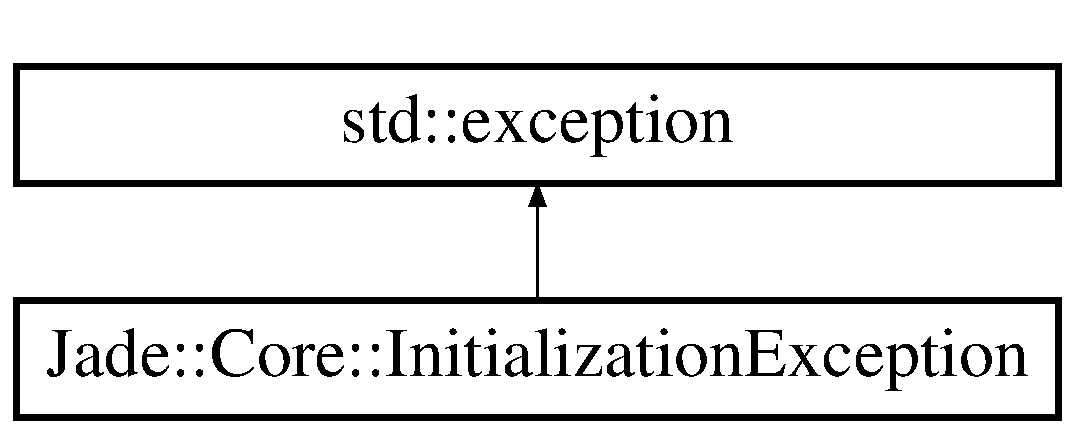
\includegraphics[height=2.000000cm]{class_jade_1_1_core_1_1_initialization_exception}
\end{center}
\end{figure}
\subsection*{Public Member Functions}
\begin{DoxyCompactItemize}
\item 
\hypertarget{class_jade_1_1_core_1_1_initialization_exception_ac5f8c44049f3c21b91cf7fd101dd0832}{}{\bfseries Initialization\+Exception} (std\+::string message)\label{class_jade_1_1_core_1_1_initialization_exception_ac5f8c44049f3c21b91cf7fd101dd0832}

\item 
\hypertarget{class_jade_1_1_core_1_1_initialization_exception_a7ed1653564bf8c76baad021bd1929ccc}{}const char $\ast$ {\bfseries what} () const  override  throw ()\label{class_jade_1_1_core_1_1_initialization_exception_a7ed1653564bf8c76baad021bd1929ccc}

\end{DoxyCompactItemize}


The documentation for this class was generated from the following file\+:\begin{DoxyCompactItemize}
\item 
C\+:/\+Users/\+Ben/\+Documents/\+Git\+Hub/\+Jade/\+Jade/\+Source/\+Core/\+Exception/Initialization\+Exception.\+h\end{DoxyCompactItemize}

\hypertarget{struct_jade_1_1_input_1_1_input}{}\section{Jade\+:\+:Input\+:\+:Input Struct Reference}
\label{struct_jade_1_1_input_1_1_input}\index{Jade\+::\+Input\+::\+Input@{Jade\+::\+Input\+::\+Input}}
\subsection*{Public Attributes}
\begin{DoxyCompactItemize}
\item 
\hypertarget{struct_jade_1_1_input_1_1_input_aca95e2a903215ba70da065dccc7e31a4}{}\hyperlink{class_jade_1_1_input_1_1_keyboard}{Keyboard} {\bfseries keyboard}\label{struct_jade_1_1_input_1_1_input_aca95e2a903215ba70da065dccc7e31a4}

\item 
\hypertarget{struct_jade_1_1_input_1_1_input_a00a7550d803462e03f3e6984a351d130}{}\hyperlink{class_jade_1_1_input_1_1_mouse}{Mouse} {\bfseries mouse}\label{struct_jade_1_1_input_1_1_input_a00a7550d803462e03f3e6984a351d130}

\end{DoxyCompactItemize}


The documentation for this struct was generated from the following file\+:\begin{DoxyCompactItemize}
\item 
C\+:/\+Users/\+Ben/\+Documents/\+Git\+Hub/\+Jade/\+Jade/\+Source/\+Input/Input.\+h\end{DoxyCompactItemize}

\hypertarget{struct_jade_1_1_graphics_1_1_i_rasterizer}{}\section{Jade\+:\+:Graphics\+:\+:I\+Rasterizer Struct Reference}
\label{struct_jade_1_1_graphics_1_1_i_rasterizer}\index{Jade\+::\+Graphics\+::\+I\+Rasterizer@{Jade\+::\+Graphics\+::\+I\+Rasterizer}}
Inheritance diagram for Jade\+:\+:Graphics\+:\+:I\+Rasterizer\+:\begin{figure}[H]
\begin{center}
\leavevmode
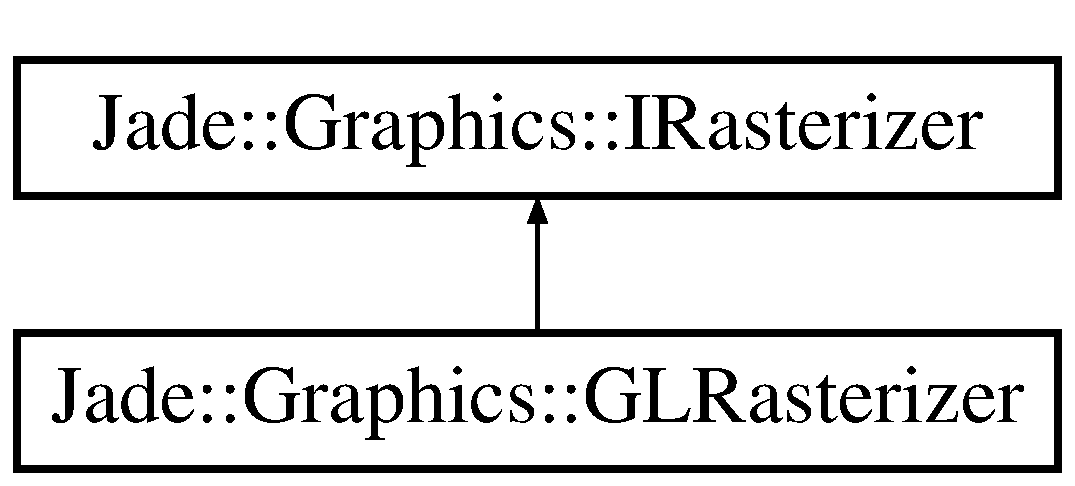
\includegraphics[height=2.000000cm]{struct_jade_1_1_graphics_1_1_i_rasterizer}
\end{center}
\end{figure}
\subsection*{Public Member Functions}
\begin{DoxyCompactItemize}
\item 
\hypertarget{struct_jade_1_1_graphics_1_1_i_rasterizer_a4063c858e345ceaca3ce995af411c4d0}{}virtual bool {\bfseries Set\+Rasterizer\+State} (Cull\+Mode cull\+Mode, Fill\+Mode fill\+Mode)=0\label{struct_jade_1_1_graphics_1_1_i_rasterizer_a4063c858e345ceaca3ce995af411c4d0}

\end{DoxyCompactItemize}


The documentation for this struct was generated from the following file\+:\begin{DoxyCompactItemize}
\item 
C\+:/\+Users/\+Ben/\+Documents/\+Git\+Hub/\+Jade/\+Jade/\+Source/\+Graphics/\+Rasterizer/I\+Rasterizer.\+h\end{DoxyCompactItemize}

\hypertarget{struct_jade_1_1_graphics_1_1_i_shader}{}\section{Jade\+:\+:Graphics\+:\+:I\+Shader Struct Reference}
\label{struct_jade_1_1_graphics_1_1_i_shader}\index{Jade\+::\+Graphics\+::\+I\+Shader@{Jade\+::\+Graphics\+::\+I\+Shader}}
Inheritance diagram for Jade\+:\+:Graphics\+:\+:I\+Shader\+:\begin{figure}[H]
\begin{center}
\leavevmode
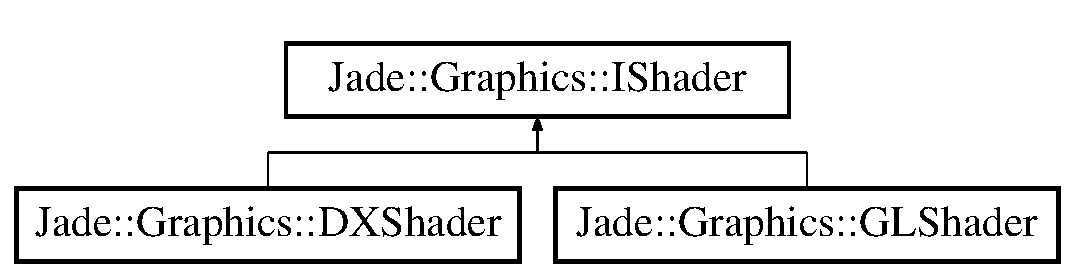
\includegraphics[height=2.000000cm]{struct_jade_1_1_graphics_1_1_i_shader}
\end{center}
\end{figure}
\subsection*{Public Member Functions}
\begin{DoxyCompactItemize}
\item 
\hypertarget{struct_jade_1_1_graphics_1_1_i_shader_a0c7e4a24b2618363efb6eb11442f7589}{}virtual void {\bfseries Make\+Active} ()=0\label{struct_jade_1_1_graphics_1_1_i_shader_a0c7e4a24b2618363efb6eb11442f7589}

\end{DoxyCompactItemize}


The documentation for this struct was generated from the following file\+:\begin{DoxyCompactItemize}
\item 
C\+:/\+Users/\+Ben/\+Documents/\+Git\+Hub/\+Jade/\+Jade/\+Source/\+Graphics/\+Shader/I\+Shader.\+h\end{DoxyCompactItemize}

\hypertarget{struct_jade_1_1_graphics_1_1_i_texture}{}\section{Jade\+:\+:Graphics\+:\+:I\+Texture Struct Reference}
\label{struct_jade_1_1_graphics_1_1_i_texture}\index{Jade\+::\+Graphics\+::\+I\+Texture@{Jade\+::\+Graphics\+::\+I\+Texture}}
\subsection*{Public Member Functions}
\begin{DoxyCompactItemize}
\item 
\hypertarget{struct_jade_1_1_graphics_1_1_i_texture_af55656b5b19dc7c930498cd657e5a71f}{}virtual bool {\bfseries Create\+Texture\+From\+File} ()=0\label{struct_jade_1_1_graphics_1_1_i_texture_af55656b5b19dc7c930498cd657e5a71f}

\item 
\hypertarget{struct_jade_1_1_graphics_1_1_i_texture_a5f13651306a080d172402bf3c3816467}{}virtual bool {\bfseries Create\+Texture\+From\+Memory} ()=0\label{struct_jade_1_1_graphics_1_1_i_texture_a5f13651306a080d172402bf3c3816467}

\end{DoxyCompactItemize}


The documentation for this struct was generated from the following file\+:\begin{DoxyCompactItemize}
\item 
C\+:/\+Users/\+Ben/\+Documents/\+Git\+Hub/\+Jade/\+Jade/\+Source/\+Graphics/\+Texture/I\+Texture.\+h\end{DoxyCompactItemize}

\hypertarget{struct_jade_1_1_graphics_1_1_i_vertex_buffer}{}\section{Jade\+:\+:Graphics\+:\+:I\+Vertex\+Buffer Struct Reference}
\label{struct_jade_1_1_graphics_1_1_i_vertex_buffer}\index{Jade\+::\+Graphics\+::\+I\+Vertex\+Buffer@{Jade\+::\+Graphics\+::\+I\+Vertex\+Buffer}}
Inheritance diagram for Jade\+:\+:Graphics\+:\+:I\+Vertex\+Buffer\+:\begin{figure}[H]
\begin{center}
\leavevmode
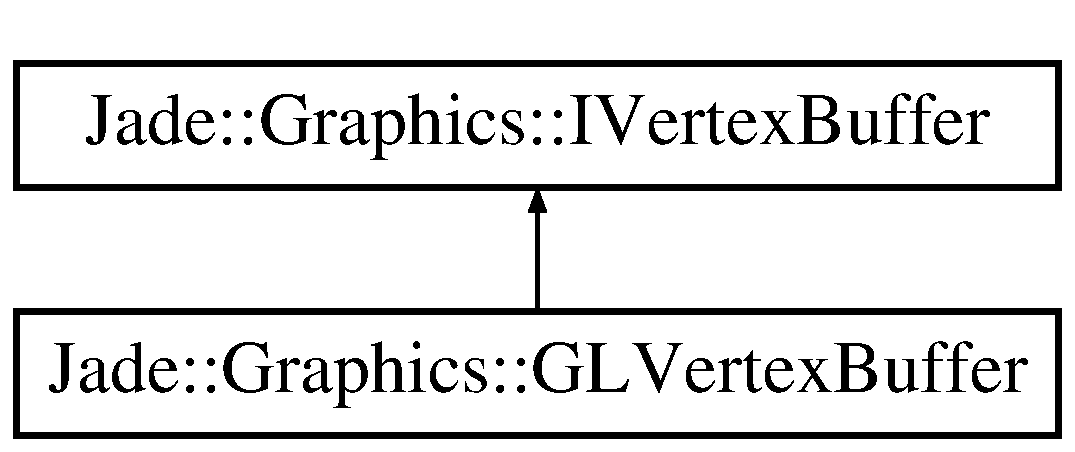
\includegraphics[height=2.000000cm]{struct_jade_1_1_graphics_1_1_i_vertex_buffer}
\end{center}
\end{figure}
\subsection*{Public Member Functions}
\begin{DoxyCompactItemize}
\item 
\hypertarget{struct_jade_1_1_graphics_1_1_i_vertex_buffer_a9b715c32b88c9825b143cae785cd36df}{}virtual void {\bfseries Bind} ()=0\label{struct_jade_1_1_graphics_1_1_i_vertex_buffer_a9b715c32b88c9825b143cae785cd36df}

\item 
\hypertarget{struct_jade_1_1_graphics_1_1_i_vertex_buffer_a11bdde3c98e13758b261de9c7b9ccc17}{}virtual bool {\bfseries Create} ()=0\label{struct_jade_1_1_graphics_1_1_i_vertex_buffer_a11bdde3c98e13758b261de9c7b9ccc17}

\item 
\hypertarget{struct_jade_1_1_graphics_1_1_i_vertex_buffer_a2c3432b5a173d533a9d4d22ccdde8c25}{}virtual std\+::vector$<$ \hyperlink{struct_jade_1_1_math_1_1_vertex}{Math\+::\+Vertex} $>$ {\bfseries Get\+Vertices} ()=0\label{struct_jade_1_1_graphics_1_1_i_vertex_buffer_a2c3432b5a173d533a9d4d22ccdde8c25}

\item 
\hypertarget{struct_jade_1_1_graphics_1_1_i_vertex_buffer_a12d631e9c2f6b0270fc3d727933a538e}{}virtual void {\bfseries Set\+Vertices} (std\+::vector$<$ \hyperlink{struct_jade_1_1_math_1_1_vertex}{Math\+::\+Vertex} $>$ vertices)=0\label{struct_jade_1_1_graphics_1_1_i_vertex_buffer_a12d631e9c2f6b0270fc3d727933a538e}

\item 
\hypertarget{struct_jade_1_1_graphics_1_1_i_vertex_buffer_a7352d3a1aed4d79a200cec3f1b7a77d7}{}virtual void {\bfseries Unbind} ()=0\label{struct_jade_1_1_graphics_1_1_i_vertex_buffer_a7352d3a1aed4d79a200cec3f1b7a77d7}

\item 
\hypertarget{struct_jade_1_1_graphics_1_1_i_vertex_buffer_a09a901410d43406272907cce3f8f67d5}{}virtual void {\bfseries Update} ()=0\label{struct_jade_1_1_graphics_1_1_i_vertex_buffer_a09a901410d43406272907cce3f8f67d5}

\end{DoxyCompactItemize}


The documentation for this struct was generated from the following file\+:\begin{DoxyCompactItemize}
\item 
C\+:/\+Users/\+Ben/\+Documents/\+Git\+Hub/\+Jade/\+Jade/\+Source/\+Graphics/\+Buffer/I\+Vertex\+Buffer.\+h\end{DoxyCompactItemize}

\hypertarget{struct_jade_1_1_system_1_1_i_window}{}\section{Jade\+:\+:System\+:\+:I\+Window Struct Reference}
\label{struct_jade_1_1_system_1_1_i_window}\index{Jade\+::\+System\+::\+I\+Window@{Jade\+::\+System\+::\+I\+Window}}
Inheritance diagram for Jade\+:\+:System\+:\+:I\+Window\+:\begin{figure}[H]
\begin{center}
\leavevmode
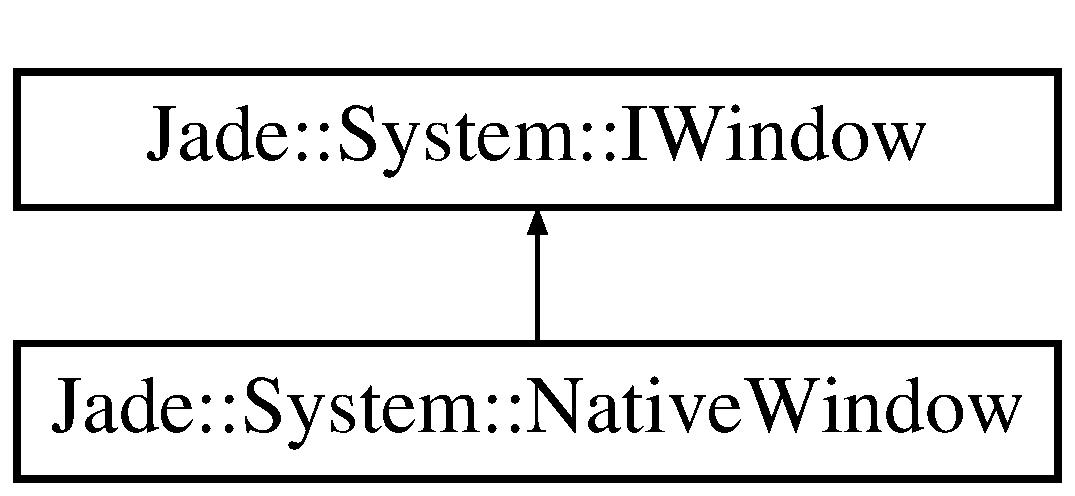
\includegraphics[height=2.000000cm]{struct_jade_1_1_system_1_1_i_window}
\end{center}
\end{figure}
\subsection*{Public Member Functions}
\begin{DoxyCompactItemize}
\item 
\hypertarget{struct_jade_1_1_system_1_1_i_window_a6e039061e47c6d533e7aae7e3335aeff}{}virtual int {\bfseries Get\+Width} ()=0\label{struct_jade_1_1_system_1_1_i_window_a6e039061e47c6d533e7aae7e3335aeff}

\item 
\hypertarget{struct_jade_1_1_system_1_1_i_window_ae5294c899b398a8efe912c06f5eda0ec}{}virtual void {\bfseries Set\+Width} (int value)=0\label{struct_jade_1_1_system_1_1_i_window_ae5294c899b398a8efe912c06f5eda0ec}

\item 
\hypertarget{struct_jade_1_1_system_1_1_i_window_acec7abf3182935e654dd9e8271c6e2b5}{}virtual int {\bfseries Get\+Height} ()=0\label{struct_jade_1_1_system_1_1_i_window_acec7abf3182935e654dd9e8271c6e2b5}

\item 
\hypertarget{struct_jade_1_1_system_1_1_i_window_acd96618872a2a2b8f195c2cc5b19ac9e}{}virtual void {\bfseries Set\+Height} (int value)=0\label{struct_jade_1_1_system_1_1_i_window_acd96618872a2a2b8f195c2cc5b19ac9e}

\item 
\hypertarget{struct_jade_1_1_system_1_1_i_window_a6def5292c72237c393577207c5a8f907}{}virtual float {\bfseries Get\+Aspect\+Ratio} ()=0\label{struct_jade_1_1_system_1_1_i_window_a6def5292c72237c393577207c5a8f907}

\item 
\hypertarget{struct_jade_1_1_system_1_1_i_window_a1bad223d4ed74c9014a06ddf4bf9b583}{}virtual int {\bfseries Get\+X} ()=0\label{struct_jade_1_1_system_1_1_i_window_a1bad223d4ed74c9014a06ddf4bf9b583}

\item 
\hypertarget{struct_jade_1_1_system_1_1_i_window_a84c1ffac1f65157d9d94bf94679ed21d}{}virtual void {\bfseries Set\+X} (int value)=0\label{struct_jade_1_1_system_1_1_i_window_a84c1ffac1f65157d9d94bf94679ed21d}

\item 
\hypertarget{struct_jade_1_1_system_1_1_i_window_ab09f4572cfcb28360160824af3cb7d5e}{}virtual int {\bfseries Get\+Y} ()=0\label{struct_jade_1_1_system_1_1_i_window_ab09f4572cfcb28360160824af3cb7d5e}

\item 
\hypertarget{struct_jade_1_1_system_1_1_i_window_a638ac54cc8c927a7f2aa02c5e0a9088c}{}virtual void {\bfseries Set\+Y} (int value)=0\label{struct_jade_1_1_system_1_1_i_window_a638ac54cc8c927a7f2aa02c5e0a9088c}

\item 
\hypertarget{struct_jade_1_1_system_1_1_i_window_a70c6852ee995e25919975b390d2471ea}{}virtual std\+::string {\bfseries Get\+Title} ()=0\label{struct_jade_1_1_system_1_1_i_window_a70c6852ee995e25919975b390d2471ea}

\item 
\hypertarget{struct_jade_1_1_system_1_1_i_window_a73e658c6cbde5d24393a5e6b7eba7a89}{}virtual void {\bfseries Set\+Title} (std\+::string value)=0\label{struct_jade_1_1_system_1_1_i_window_a73e658c6cbde5d24393a5e6b7eba7a89}

\item 
\hypertarget{struct_jade_1_1_system_1_1_i_window_aaf65dcd80219f81971e6df332e287ca7}{}virtual \hyperlink{class_jade_1_1_math_1_1_point}{Math\+::\+Point} {\bfseries Get\+Position} ()=0\label{struct_jade_1_1_system_1_1_i_window_aaf65dcd80219f81971e6df332e287ca7}

\item 
\hypertarget{struct_jade_1_1_system_1_1_i_window_ab2ac292666b47abc176ee06555ec408a}{}virtual void {\bfseries Set\+Position} (int x, int y)=0\label{struct_jade_1_1_system_1_1_i_window_ab2ac292666b47abc176ee06555ec408a}

\item 
\hypertarget{struct_jade_1_1_system_1_1_i_window_a2eb7b946f98f26b6a96bda0a86d613c3}{}virtual void {\bfseries Set\+Icon} (std\+::string filename)=0\label{struct_jade_1_1_system_1_1_i_window_a2eb7b946f98f26b6a96bda0a86d613c3}

\item 
\hypertarget{struct_jade_1_1_system_1_1_i_window_a7b60d7548c9fb03537b56ab3adc10248}{}virtual bool {\bfseries Poll\+Window\+Events} ()=0\label{struct_jade_1_1_system_1_1_i_window_a7b60d7548c9fb03537b56ab3adc10248}

\item 
\hypertarget{struct_jade_1_1_system_1_1_i_window_a6de41f70337a08edc07dcbe0fef09851}{}virtual void {\bfseries Close} ()=0\label{struct_jade_1_1_system_1_1_i_window_a6de41f70337a08edc07dcbe0fef09851}

\item 
\hypertarget{struct_jade_1_1_system_1_1_i_window_a39fa1e856f35bbca63780d84601da47f}{}virtual void $\ast$ {\bfseries Handle} ()=0\label{struct_jade_1_1_system_1_1_i_window_a39fa1e856f35bbca63780d84601da47f}

\item 
\hypertarget{struct_jade_1_1_system_1_1_i_window_abdae35c83a2ca0bf26b6d4f7eb4926c6}{}virtual bool {\bfseries Init\+Window} ()=0\label{struct_jade_1_1_system_1_1_i_window_abdae35c83a2ca0bf26b6d4f7eb4926c6}

\item 
\hypertarget{struct_jade_1_1_system_1_1_i_window_a643fd6ea7e006923a945c1307d6be267}{}virtual void {\bfseries Show} ()=0\label{struct_jade_1_1_system_1_1_i_window_a643fd6ea7e006923a945c1307d6be267}

\item 
\hypertarget{struct_jade_1_1_system_1_1_i_window_a3a66cdae81b5254fd255e841af0d3d57}{}virtual void {\bfseries Hide} ()=0\label{struct_jade_1_1_system_1_1_i_window_a3a66cdae81b5254fd255e841af0d3d57}

\item 
\hypertarget{struct_jade_1_1_system_1_1_i_window_a88639ad2ce017e15c61aa2fdfa5c5d52}{}virtual void {\bfseries Restore} ()=0\label{struct_jade_1_1_system_1_1_i_window_a88639ad2ce017e15c61aa2fdfa5c5d52}

\item 
\hypertarget{struct_jade_1_1_system_1_1_i_window_a3f4acb7462be46b808e5099493683054}{}virtual void {\bfseries Maximize} ()=0\label{struct_jade_1_1_system_1_1_i_window_a3f4acb7462be46b808e5099493683054}

\item 
\hypertarget{struct_jade_1_1_system_1_1_i_window_a008ef55b26224bd95b46b1319ddb5914}{}virtual bool {\bfseries Is\+Minimized} ()=0\label{struct_jade_1_1_system_1_1_i_window_a008ef55b26224bd95b46b1319ddb5914}

\item 
\hypertarget{struct_jade_1_1_system_1_1_i_window_aa237b7dbadd43f2baf2fec704ee4ee38}{}virtual void {\bfseries Minimize} ()=0\label{struct_jade_1_1_system_1_1_i_window_aa237b7dbadd43f2baf2fec704ee4ee38}

\item 
\hypertarget{struct_jade_1_1_system_1_1_i_window_a38470abade82778582f529c3eabe4fe0}{}virtual bool {\bfseries Is\+Maximized} ()=0\label{struct_jade_1_1_system_1_1_i_window_a38470abade82778582f529c3eabe4fe0}

\item 
\hypertarget{struct_jade_1_1_system_1_1_i_window_a68f6d58c9e450bf837a5099c44ce8adf}{}virtual bool {\bfseries Is\+Visible} ()=0\label{struct_jade_1_1_system_1_1_i_window_a68f6d58c9e450bf837a5099c44ce8adf}

\item 
\hypertarget{struct_jade_1_1_system_1_1_i_window_a334e475db667839044a87d17452c85e8}{}virtual bool {\bfseries Is\+Open} ()=0\label{struct_jade_1_1_system_1_1_i_window_a334e475db667839044a87d17452c85e8}

\item 
\hypertarget{struct_jade_1_1_system_1_1_i_window_a1431c2abbaf150947bbd2321d194c298}{}virtual bool {\bfseries Is\+Fullscreen} ()=0\label{struct_jade_1_1_system_1_1_i_window_a1431c2abbaf150947bbd2321d194c298}

\item 
\hypertarget{struct_jade_1_1_system_1_1_i_window_a2ed18cb232956c62866a853c7f99355d}{}virtual bool {\bfseries Is\+Active} ()=0\label{struct_jade_1_1_system_1_1_i_window_a2ed18cb232956c62866a853c7f99355d}

\item 
\hypertarget{struct_jade_1_1_system_1_1_i_window_a7ec89541f3839eba001150de210d365a}{}virtual \hyperlink{class_jade_1_1_core_1_1_time}{Core\+::\+Time} {\bfseries Get\+Time} ()=0\label{struct_jade_1_1_system_1_1_i_window_a7ec89541f3839eba001150de210d365a}

\item 
\hypertarget{struct_jade_1_1_system_1_1_i_window_a117186f37258b80db6018f87ee0ae9dd}{}virtual \hyperlink{struct_jade_1_1_core_1_1_input}{Core\+::\+Input} {\bfseries Get\+Input} ()=0\label{struct_jade_1_1_system_1_1_i_window_a117186f37258b80db6018f87ee0ae9dd}

\end{DoxyCompactItemize}


The documentation for this struct was generated from the following file\+:\begin{DoxyCompactItemize}
\item 
C\+:/\+Users/\+Ben/\+Documents/\+Git\+Hub/\+Jade/\+Jade/\+Source/\+System/\+Window/I\+Window.\+h\end{DoxyCompactItemize}

\hypertarget{class_jade_1_1_input_1_1_keyboard}{}\section{Jade\+:\+:Input\+:\+:Keyboard Class Reference}
\label{class_jade_1_1_input_1_1_keyboard}\index{Jade\+::\+Input\+::\+Keyboard@{Jade\+::\+Input\+::\+Keyboard}}
\subsection*{Public Member Functions}
\begin{DoxyCompactItemize}
\item 
\hypertarget{class_jade_1_1_input_1_1_keyboard_abaf81f9db47f2b5e4e3a571330b24e93}{}bool {\bfseries Is\+Key\+Up} (Key key)\label{class_jade_1_1_input_1_1_keyboard_abaf81f9db47f2b5e4e3a571330b24e93}

\item 
\hypertarget{class_jade_1_1_input_1_1_keyboard_a65572b44109b1567626f2cc205059ba8}{}bool {\bfseries Is\+Key\+Down} (Key key)\label{class_jade_1_1_input_1_1_keyboard_a65572b44109b1567626f2cc205059ba8}

\item 
\hypertarget{class_jade_1_1_input_1_1_keyboard_a01b1e08a3c7bd4c7a7de7e4022625caa}{}std\+::vector$<$ Key $>$ {\bfseries Get\+Keys\+Pressed} ()\label{class_jade_1_1_input_1_1_keyboard_a01b1e08a3c7bd4c7a7de7e4022625caa}

\item 
\hypertarget{class_jade_1_1_input_1_1_keyboard_af036a724df0841b08ef85ab304afe6b3}{}void {\bfseries Set\+Key\+State} (Key key, Input\+State state)\label{class_jade_1_1_input_1_1_keyboard_af036a724df0841b08ef85ab304afe6b3}

\end{DoxyCompactItemize}


The documentation for this class was generated from the following files\+:\begin{DoxyCompactItemize}
\item 
C\+:/\+Users/\+Ben/\+Documents/\+Git\+Hub/\+Jade/\+Jade/\+Source/\+Input/Keyboard.\+h\item 
C\+:/\+Users/\+Ben/\+Documents/\+Git\+Hub/\+Jade/\+Jade/\+Source/\+Input/Keyboard.\+cpp\end{DoxyCompactItemize}

\hypertarget{class_jade_1_1_system_1_1_log}{}\section{Jade\+:\+:System\+:\+:Log Class Reference}
\label{class_jade_1_1_system_1_1_log}\index{Jade\+::\+System\+::\+Log@{Jade\+::\+System\+::\+Log}}
\subsection*{Public Member Functions}
\begin{DoxyCompactItemize}
\item 
\hypertarget{class_jade_1_1_system_1_1_log_a0ae495557ee5be6096556c2ea5d7480c}{}void {\bfseries Write} (std\+::string text)\label{class_jade_1_1_system_1_1_log_a0ae495557ee5be6096556c2ea5d7480c}

\end{DoxyCompactItemize}


The documentation for this class was generated from the following files\+:\begin{DoxyCompactItemize}
\item 
C\+:/\+Users/\+Ben/\+Documents/\+Git\+Hub/\+Jade/\+Jade/\+Source/\+System/Log.\+h\item 
C\+:/\+Users/\+Ben/\+Documents/\+Git\+Hub/\+Jade/\+Jade/\+Source/\+System/Log.\+cpp\end{DoxyCompactItemize}

\hypertarget{class_jade_1_1_math_1_1_math}{}\section{Jade\+:\+:Math\+:\+:Math Class Reference}
\label{class_jade_1_1_math_1_1_math}\index{Jade\+::\+Math\+::\+Math@{Jade\+::\+Math\+::\+Math}}
\subsection*{Static Public Member Functions}
\begin{DoxyCompactItemize}
\item 
\hypertarget{class_jade_1_1_math_1_1_math_aa3bdd4851ec832772ad60b305bf65d59}{}static float {\bfseries Min} (float x, float y)\label{class_jade_1_1_math_1_1_math_aa3bdd4851ec832772ad60b305bf65d59}

\item 
\hypertarget{class_jade_1_1_math_1_1_math_a7987b2173867b9b819f7c45885f5d82c}{}static float {\bfseries Max} (float x, float y)\label{class_jade_1_1_math_1_1_math_a7987b2173867b9b819f7c45885f5d82c}

\item 
\hypertarget{class_jade_1_1_math_1_1_math_a551d0bcc4301eb52c19634cc953c8cff}{}static float {\bfseries Sqrt} (float x)\label{class_jade_1_1_math_1_1_math_a551d0bcc4301eb52c19634cc953c8cff}

\item 
\hypertarget{class_jade_1_1_math_1_1_math_ad41fbf7624c853027b90901945f4c9f7}{}static float {\bfseries Inv\+Sqrt} (float x)\label{class_jade_1_1_math_1_1_math_ad41fbf7624c853027b90901945f4c9f7}

\item 
\hypertarget{class_jade_1_1_math_1_1_math_a3ee50eb9d237aeeb6a90ea0d60cc499d}{}static float {\bfseries A\+Sin} (float a)\label{class_jade_1_1_math_1_1_math_a3ee50eb9d237aeeb6a90ea0d60cc499d}

\item 
\hypertarget{class_jade_1_1_math_1_1_math_a863e6bcc5d3100fc23d18ac6a6cc1233}{}static float {\bfseries Sin} (float a)\label{class_jade_1_1_math_1_1_math_a863e6bcc5d3100fc23d18ac6a6cc1233}

\item 
\hypertarget{class_jade_1_1_math_1_1_math_a5157d7c0f20fd993d698af51fb8d82a8}{}static float {\bfseries A\+Cos} (float a)\label{class_jade_1_1_math_1_1_math_a5157d7c0f20fd993d698af51fb8d82a8}

\item 
\hypertarget{class_jade_1_1_math_1_1_math_a3ba179503e6682f8d8411f2da7986af0}{}static float {\bfseries Cos} (float a)\label{class_jade_1_1_math_1_1_math_a3ba179503e6682f8d8411f2da7986af0}

\item 
\hypertarget{class_jade_1_1_math_1_1_math_a3eafcc411a389707a5a7d8ca895ea684}{}static float {\bfseries A\+Tan} (float a)\label{class_jade_1_1_math_1_1_math_a3eafcc411a389707a5a7d8ca895ea684}

\item 
\hypertarget{class_jade_1_1_math_1_1_math_adc8931d197b3c8c3f5f5c478fe0e310c}{}static float {\bfseries Tan} (float a)\label{class_jade_1_1_math_1_1_math_adc8931d197b3c8c3f5f5c478fe0e310c}

\item 
\hypertarget{class_jade_1_1_math_1_1_math_a6dffaca84a57f964ad1704873a1908a8}{}static float {\bfseries Pow} (float x, float y)\label{class_jade_1_1_math_1_1_math_a6dffaca84a57f964ad1704873a1908a8}

\item 
\hypertarget{class_jade_1_1_math_1_1_math_a57a5db205c2fe696d01227f497589694}{}static float {\bfseries Exp} (float x)\label{class_jade_1_1_math_1_1_math_a57a5db205c2fe696d01227f497589694}

\item 
\hypertarget{class_jade_1_1_math_1_1_math_a31655f598ee80904a5041f4a66c9b7d1}{}static float {\bfseries Log} (float x)\label{class_jade_1_1_math_1_1_math_a31655f598ee80904a5041f4a66c9b7d1}

\item 
\hypertarget{class_jade_1_1_math_1_1_math_ae66af6a1b131a2098989df688bc1c7e7}{}static float {\bfseries Log10} (float x)\label{class_jade_1_1_math_1_1_math_ae66af6a1b131a2098989df688bc1c7e7}

\item 
\hypertarget{class_jade_1_1_math_1_1_math_ac32dfb7a32c05fc93723f7603e85c0b9}{}static float {\bfseries Abs} (float x)\label{class_jade_1_1_math_1_1_math_ac32dfb7a32c05fc93723f7603e85c0b9}

\item 
\hypertarget{class_jade_1_1_math_1_1_math_afe16745ed5df71eb03afa85c96f41a8f}{}static float {\bfseries Remainder} (float x, float y)\label{class_jade_1_1_math_1_1_math_afe16745ed5df71eb03afa85c96f41a8f}

\item 
\hypertarget{class_jade_1_1_math_1_1_math_a122e6605d252e605c2ff9e076e7ae7bd}{}static float {\bfseries Round} (float x)\label{class_jade_1_1_math_1_1_math_a122e6605d252e605c2ff9e076e7ae7bd}

\item 
\hypertarget{class_jade_1_1_math_1_1_math_a495b05e63389a95e70a05884314638b8}{}static int {\bfseries Random} ()\label{class_jade_1_1_math_1_1_math_a495b05e63389a95e70a05884314638b8}

\item 
\hypertarget{class_jade_1_1_math_1_1_math_acd68cb76d88b962d51b25332f7bea61d}{}static float {\bfseries Floor} (float x)\label{class_jade_1_1_math_1_1_math_acd68cb76d88b962d51b25332f7bea61d}

\item 
\hypertarget{class_jade_1_1_math_1_1_math_a75b2a6c69bce01a5e6949dc677b563de}{}static float {\bfseries Ceiling} (float x)\label{class_jade_1_1_math_1_1_math_a75b2a6c69bce01a5e6949dc677b563de}

\item 
\hypertarget{class_jade_1_1_math_1_1_math_a2208198c2e42102c6c5ccb11303a55c3}{}static bool {\bfseries Is\+Nan} (float x)\label{class_jade_1_1_math_1_1_math_a2208198c2e42102c6c5ccb11303a55c3}

\end{DoxyCompactItemize}
\subsection*{Static Public Attributes}
\begin{DoxyCompactItemize}
\item 
\hypertarget{class_jade_1_1_math_1_1_math_aa4783d6e94daa65971af2a6083aa0e34}{}static const float {\bfseries Pi} = 3.\+14159265359f\label{class_jade_1_1_math_1_1_math_aa4783d6e94daa65971af2a6083aa0e34}

\item 
\hypertarget{class_jade_1_1_math_1_1_math_a504d91ccd24079aac65abf030e624d33}{}static const float {\bfseries Two\+Pi} = 6.\+28318530718f\label{class_jade_1_1_math_1_1_math_a504d91ccd24079aac65abf030e624d33}

\item 
\hypertarget{class_jade_1_1_math_1_1_math_a1e7da29eb5899a70b57ee363ee376adc}{}static const float {\bfseries Pi\+Over\+Two} = 1.\+57079632679f\label{class_jade_1_1_math_1_1_math_a1e7da29eb5899a70b57ee363ee376adc}

\item 
\hypertarget{class_jade_1_1_math_1_1_math_af9a8a8c8fc5705196e27379f5191b732}{}static const float {\bfseries E} = 2.\+71828182845f\label{class_jade_1_1_math_1_1_math_af9a8a8c8fc5705196e27379f5191b732}

\item 
\hypertarget{class_jade_1_1_math_1_1_math_a7abe61f38af714e22baebd5d09aa7549}{}static const float {\bfseries Epsilon} = 0.\+00000000001f\label{class_jade_1_1_math_1_1_math_a7abe61f38af714e22baebd5d09aa7549}

\item 
\hypertarget{class_jade_1_1_math_1_1_math_ab14316866c81009fa35ce450b319b9e0}{}static const float {\bfseries Deg2\+Rad} = Math\+::\+Pi / 180.\+0f\label{class_jade_1_1_math_1_1_math_ab14316866c81009fa35ce450b319b9e0}

\item 
\hypertarget{class_jade_1_1_math_1_1_math_ac5850dc52c0c262a4fbfbd3652e68ccb}{}static const float {\bfseries Rad2\+Deg} = 180.\+0f / Math\+::\+Pi\label{class_jade_1_1_math_1_1_math_ac5850dc52c0c262a4fbfbd3652e68ccb}

\end{DoxyCompactItemize}


The documentation for this class was generated from the following files\+:\begin{DoxyCompactItemize}
\item 
C\+:/\+Users/\+Ben/\+Documents/\+Git\+Hub/\+Jade/\+Jade/\+Source/\+Math/Math.\+h\item 
C\+:/\+Users/\+Ben/\+Documents/\+Git\+Hub/\+Jade/\+Jade/\+Source/\+Math/Math.\+cpp\end{DoxyCompactItemize}

\hypertarget{struct_jade_1_1_math_1_1_matrix}{}\section{Jade\+:\+:Math\+:\+:Matrix Struct Reference}
\label{struct_jade_1_1_math_1_1_matrix}\index{Jade\+::\+Math\+::\+Matrix@{Jade\+::\+Math\+::\+Matrix}}
\subsection*{Public Member Functions}
\begin{DoxyCompactItemize}
\item 
\hypertarget{struct_jade_1_1_math_1_1_matrix_a1c9fccf66e7b1c1342513dba15cb5bda}{}\hyperlink{struct_jade_1_1_math_1_1_matrix}{Matrix} {\bfseries operator+} (\hyperlink{struct_jade_1_1_math_1_1_matrix}{Matrix} matrix) const \label{struct_jade_1_1_math_1_1_matrix_a1c9fccf66e7b1c1342513dba15cb5bda}

\item 
\hypertarget{struct_jade_1_1_math_1_1_matrix_aa298abd956e6475c098f6c6a15ad4f46}{}\hyperlink{struct_jade_1_1_math_1_1_matrix}{Matrix} {\bfseries operator-\/} (\hyperlink{struct_jade_1_1_math_1_1_matrix}{Matrix} matrix) const \label{struct_jade_1_1_math_1_1_matrix_aa298abd956e6475c098f6c6a15ad4f46}

\item 
\hypertarget{struct_jade_1_1_math_1_1_matrix_a650e8d6309890483dd1cac8501a6bc8a}{}\hyperlink{struct_jade_1_1_math_1_1_matrix}{Matrix} {\bfseries operator$\ast$} (\hyperlink{struct_jade_1_1_math_1_1_matrix}{Matrix} matrix) const \label{struct_jade_1_1_math_1_1_matrix_a650e8d6309890483dd1cac8501a6bc8a}

\item 
\hypertarget{struct_jade_1_1_math_1_1_matrix_a4568fc14ba54c95f6b7b13a9485622cb}{}\hyperlink{struct_jade_1_1_math_1_1_matrix}{Matrix} {\bfseries operator/} (\hyperlink{struct_jade_1_1_math_1_1_matrix}{Matrix} matrix) const \label{struct_jade_1_1_math_1_1_matrix_a4568fc14ba54c95f6b7b13a9485622cb}

\item 
\hypertarget{struct_jade_1_1_math_1_1_matrix_a114c08bf64318686c8cc5aa463ebe638}{}{\bfseries Matrix} (float m00, float m01, float m02, float m03, float m10, float m11, float m12, float m13, float m20, float m21, float m22, float m23, float m30, float m31, float m32, float m33)\label{struct_jade_1_1_math_1_1_matrix_a114c08bf64318686c8cc5aa463ebe638}

\item 
\hypertarget{struct_jade_1_1_math_1_1_matrix_aa06e1c797c397f4ef041e0f1d9e5b572}{}\hyperlink{struct_jade_1_1_math_1_1_matrix}{Matrix} \hyperlink{struct_jade_1_1_math_1_1_matrix_aa06e1c797c397f4ef041e0f1d9e5b572}{Add} (\hyperlink{struct_jade_1_1_math_1_1_matrix}{Matrix} other) const \label{struct_jade_1_1_math_1_1_matrix_aa06e1c797c397f4ef041e0f1d9e5b572}

\begin{DoxyCompactList}\small\item\em Adds two matrices and returns a matrix as a result. \end{DoxyCompactList}\item 
\hypertarget{struct_jade_1_1_math_1_1_matrix_ad463c28a746f11e6e39bce0c3c8bae7d}{}\hyperlink{struct_jade_1_1_math_1_1_matrix}{Matrix} \hyperlink{struct_jade_1_1_math_1_1_matrix_ad463c28a746f11e6e39bce0c3c8bae7d}{Create\+Look\+At} (\hyperlink{struct_jade_1_1_math_1_1_vector3}{Vector3} eye, \hyperlink{struct_jade_1_1_math_1_1_vector3}{Vector3} at, \hyperlink{struct_jade_1_1_math_1_1_vector3}{Vector3} up)\label{struct_jade_1_1_math_1_1_matrix_ad463c28a746f11e6e39bce0c3c8bae7d}

\begin{DoxyCompactList}\small\item\em Returns a matrix with the camera vectors. \end{DoxyCompactList}\item 
\hypertarget{struct_jade_1_1_math_1_1_matrix_ae3ea05edfb34a8fef4453e96c830b994}{}\hyperlink{struct_jade_1_1_math_1_1_matrix}{Matrix} \hyperlink{struct_jade_1_1_math_1_1_matrix_ae3ea05edfb34a8fef4453e96c830b994}{Create\+Orthographic\+View} (float field\+Of\+View, float aspect\+Ratio, float near\+Plane\+Distance, float far\+Plane\+Distance)\label{struct_jade_1_1_math_1_1_matrix_ae3ea05edfb34a8fef4453e96c830b994}

\begin{DoxyCompactList}\small\item\em Returns a matrix that is of an Orthographic view. \end{DoxyCompactList}\item 
\hypertarget{struct_jade_1_1_math_1_1_matrix_a2ee438ed4038bb5565050054308c80a9}{}\hyperlink{struct_jade_1_1_math_1_1_matrix}{Matrix} \hyperlink{struct_jade_1_1_math_1_1_matrix_a2ee438ed4038bb5565050054308c80a9}{Create\+Perspective\+View} (float field\+Of\+View, float aspect\+Ratio, float near\+Plane\+Distance, float far\+Plane\+Distance)\label{struct_jade_1_1_math_1_1_matrix_a2ee438ed4038bb5565050054308c80a9}

\begin{DoxyCompactList}\small\item\em Returns a matrix that is of a Perspective view. \end{DoxyCompactList}\item 
\hypertarget{struct_jade_1_1_math_1_1_matrix_a23ed117800c7c6734930f84a7c864c1a}{}float(\& \hyperlink{struct_jade_1_1_math_1_1_matrix_a23ed117800c7c6734930f84a7c864c1a}{Data} ())\mbox{[}4\mbox{]}\label{struct_jade_1_1_math_1_1_matrix_a23ed117800c7c6734930f84a7c864c1a}

\begin{DoxyCompactList}\small\item\em Returns a reference to the raw data contained within the matrix. \end{DoxyCompactList}\item 
\hypertarget{struct_jade_1_1_math_1_1_matrix_a8b030138c16b571491ec6880269a9bed}{}float \hyperlink{struct_jade_1_1_math_1_1_matrix_a8b030138c16b571491ec6880269a9bed}{Determinant} ()\label{struct_jade_1_1_math_1_1_matrix_a8b030138c16b571491ec6880269a9bed}

\begin{DoxyCompactList}\small\item\em Returns the determinant of the matrix. \end{DoxyCompactList}\item 
\hypertarget{struct_jade_1_1_math_1_1_matrix_a6dff4eaa15baad168ba91920b1ceaf93}{}\hyperlink{struct_jade_1_1_math_1_1_matrix}{Matrix} \hyperlink{struct_jade_1_1_math_1_1_matrix_a6dff4eaa15baad168ba91920b1ceaf93}{Divide} (\hyperlink{struct_jade_1_1_math_1_1_matrix}{Matrix} other) const \label{struct_jade_1_1_math_1_1_matrix_a6dff4eaa15baad168ba91920b1ceaf93}

\begin{DoxyCompactList}\small\item\em Divides two matrices and returns a matrix as a result. \end{DoxyCompactList}\item 
\hypertarget{struct_jade_1_1_math_1_1_matrix_a922429ce3242f0df5d2987dfe7de238b}{}\hyperlink{struct_jade_1_1_math_1_1_matrix}{Matrix} \hyperlink{struct_jade_1_1_math_1_1_matrix_a922429ce3242f0df5d2987dfe7de238b}{Inverse} ()\label{struct_jade_1_1_math_1_1_matrix_a922429ce3242f0df5d2987dfe7de238b}

\begin{DoxyCompactList}\small\item\em Returns a matrix that is the inverse. \end{DoxyCompactList}\item 
\hypertarget{struct_jade_1_1_math_1_1_matrix_a449adacaa4ef60d602e95f73d0d12c8a}{}\hyperlink{struct_jade_1_1_math_1_1_matrix}{Matrix} \hyperlink{struct_jade_1_1_math_1_1_matrix_a449adacaa4ef60d602e95f73d0d12c8a}{Multiply} (\hyperlink{struct_jade_1_1_math_1_1_matrix}{Matrix} other) const \label{struct_jade_1_1_math_1_1_matrix_a449adacaa4ef60d602e95f73d0d12c8a}

\begin{DoxyCompactList}\small\item\em Multiplies two matrices and returns a matrix as a result. \end{DoxyCompactList}\item 
\hypertarget{struct_jade_1_1_math_1_1_matrix_a93092c82d04a623e9da883b5288b20b1}{}\hyperlink{struct_jade_1_1_math_1_1_matrix}{Matrix} \hyperlink{struct_jade_1_1_math_1_1_matrix_a93092c82d04a623e9da883b5288b20b1}{Negate} ()\label{struct_jade_1_1_math_1_1_matrix_a93092c82d04a623e9da883b5288b20b1}

\begin{DoxyCompactList}\small\item\em Returns a matrix with the values negated. \end{DoxyCompactList}\item 
\hypertarget{struct_jade_1_1_math_1_1_matrix_a930c8e6f7409fbab5f4d30946fc411a5}{}\hyperlink{struct_jade_1_1_math_1_1_matrix}{Matrix} \hyperlink{struct_jade_1_1_math_1_1_matrix_a930c8e6f7409fbab5f4d30946fc411a5}{Rotate\+Along\+X} (float radians) const \label{struct_jade_1_1_math_1_1_matrix_a930c8e6f7409fbab5f4d30946fc411a5}

\begin{DoxyCompactList}\small\item\em Rotates the matrix along the x-\/axis by a specified amount in radians. \end{DoxyCompactList}\item 
\hypertarget{struct_jade_1_1_math_1_1_matrix_a874b086183562b6d3c206d3aa89357a2}{}\hyperlink{struct_jade_1_1_math_1_1_matrix}{Matrix} \hyperlink{struct_jade_1_1_math_1_1_matrix_a874b086183562b6d3c206d3aa89357a2}{Rotate\+Along\+Y} (float radians) const \label{struct_jade_1_1_math_1_1_matrix_a874b086183562b6d3c206d3aa89357a2}

\begin{DoxyCompactList}\small\item\em Rotates the matrix along the y -\/ axis by a specified amount in radians. \end{DoxyCompactList}\item 
\hypertarget{struct_jade_1_1_math_1_1_matrix_a4e611999b9d39fb3027f2c9007a1f930}{}\hyperlink{struct_jade_1_1_math_1_1_matrix}{Matrix} \hyperlink{struct_jade_1_1_math_1_1_matrix_a4e611999b9d39fb3027f2c9007a1f930}{Rotate\+Along\+Z} (float radians) const \label{struct_jade_1_1_math_1_1_matrix_a4e611999b9d39fb3027f2c9007a1f930}

\begin{DoxyCompactList}\small\item\em Rotates the matrix along the z -\/ axis by a specified amount in radians. \end{DoxyCompactList}\item 
\hypertarget{struct_jade_1_1_math_1_1_matrix_af5c307e7450771500c0b1199f7f04096}{}\hyperlink{struct_jade_1_1_math_1_1_matrix}{Matrix} \hyperlink{struct_jade_1_1_math_1_1_matrix_af5c307e7450771500c0b1199f7f04096}{Subtract} (\hyperlink{struct_jade_1_1_math_1_1_matrix}{Matrix} other) const \label{struct_jade_1_1_math_1_1_matrix_af5c307e7450771500c0b1199f7f04096}

\begin{DoxyCompactList}\small\item\em Subtracts two matrices and returns a matrix as a result. \end{DoxyCompactList}\item 
\hypertarget{struct_jade_1_1_math_1_1_matrix_aa1a013157118a87cd242d25e668aa3b6}{}\hyperlink{struct_jade_1_1_math_1_1_matrix}{Matrix} \hyperlink{struct_jade_1_1_math_1_1_matrix_aa1a013157118a87cd242d25e668aa3b6}{Translate} (float x\+Offset, float y\+Offset, float z\+Offset)\label{struct_jade_1_1_math_1_1_matrix_aa1a013157118a87cd242d25e668aa3b6}

\begin{DoxyCompactList}\small\item\em Returns a matrix that is translated by the specified offsets. \end{DoxyCompactList}\item 
\hypertarget{struct_jade_1_1_math_1_1_matrix_ac235e6add4163f779f1a3b007ee0f6d7}{}\hyperlink{struct_jade_1_1_math_1_1_matrix}{Matrix} \hyperlink{struct_jade_1_1_math_1_1_matrix_ac235e6add4163f779f1a3b007ee0f6d7}{Transpose} ()\label{struct_jade_1_1_math_1_1_matrix_ac235e6add4163f779f1a3b007ee0f6d7}

\begin{DoxyCompactList}\small\item\em Returns a matrix where the rows are columns and the columns are rows. \end{DoxyCompactList}\item 
\hypertarget{struct_jade_1_1_math_1_1_matrix_a913cad2a5906c10e1547ca26a1c3f18d}{}std\+::string \hyperlink{struct_jade_1_1_math_1_1_matrix_a913cad2a5906c10e1547ca26a1c3f18d}{To\+String} ()\label{struct_jade_1_1_math_1_1_matrix_a913cad2a5906c10e1547ca26a1c3f18d}

\begin{DoxyCompactList}\small\item\em Returns a string representation of the matrix. \end{DoxyCompactList}\end{DoxyCompactItemize}
\subsection*{Static Public Attributes}
\begin{DoxyCompactItemize}
\item 
\hypertarget{struct_jade_1_1_math_1_1_matrix_a89bfcd378ee8aeba30f393a9bc431e49}{}static const \hyperlink{struct_jade_1_1_math_1_1_matrix}{Matrix} {\bfseries Identity}\label{struct_jade_1_1_math_1_1_matrix_a89bfcd378ee8aeba30f393a9bc431e49}

\item 
\hypertarget{struct_jade_1_1_math_1_1_matrix_a32ed6952707144091d2bee00c0af4cc4}{}static const \hyperlink{struct_jade_1_1_math_1_1_matrix}{Matrix} {\bfseries Zero}\label{struct_jade_1_1_math_1_1_matrix_a32ed6952707144091d2bee00c0af4cc4}

\end{DoxyCompactItemize}


The documentation for this struct was generated from the following files\+:\begin{DoxyCompactItemize}
\item 
C\+:/\+Users/\+Ben/\+Documents/\+Git\+Hub/\+Jade/\+Jade/\+Source/\+Math/Matrix.\+h\item 
C\+:/\+Users/\+Ben/\+Documents/\+Git\+Hub/\+Jade/\+Jade/\+Source/\+Math/Matrix.\+cpp\end{DoxyCompactItemize}

\hypertarget{class_jade_1_1_graphics_1_1_mesh}{}\section{Jade\+:\+:Graphics\+:\+:Mesh Class Reference}
\label{class_jade_1_1_graphics_1_1_mesh}\index{Jade\+::\+Graphics\+::\+Mesh@{Jade\+::\+Graphics\+::\+Mesh}}
\subsection*{Public Member Functions}
\begin{DoxyCompactItemize}
\item 
\hypertarget{class_jade_1_1_graphics_1_1_mesh_a7f088e578ccf88621257a1b703a83481}{}{\bfseries Mesh} (\hyperlink{class_jade_1_1_graphics_1_1_device}{Device} device, std\+::vector$<$ \hyperlink{struct_jade_1_1_math_1_1_vertex}{Math\+::\+Vertex} $>$ vertices, std\+::vector$<$ unsigned int $>$ indices)\label{class_jade_1_1_graphics_1_1_mesh_a7f088e578ccf88621257a1b703a83481}

\item 
\hypertarget{class_jade_1_1_graphics_1_1_mesh_aab6996e51de3121c2aa0630208d2c344}{}void {\bfseries Draw} () const \label{class_jade_1_1_graphics_1_1_mesh_aab6996e51de3121c2aa0630208d2c344}

\item 
\hypertarget{class_jade_1_1_graphics_1_1_mesh_a452aadf2a87307d19b088b9bc2776b07}{}void {\bfseries Bind} () const \label{class_jade_1_1_graphics_1_1_mesh_a452aadf2a87307d19b088b9bc2776b07}

\item 
\hypertarget{class_jade_1_1_graphics_1_1_mesh_aaf5c688a1cab7121aca17b87898ed8bd}{}void {\bfseries Unbind} () const \label{class_jade_1_1_graphics_1_1_mesh_aaf5c688a1cab7121aca17b87898ed8bd}

\end{DoxyCompactItemize}


The documentation for this class was generated from the following files\+:\begin{DoxyCompactItemize}
\item 
C\+:/\+Users/\+Ben/\+Documents/\+Git\+Hub/\+Jade/\+Jade/\+Source/\+Graphics/\+Mesh/Mesh.\+h\item 
C\+:/\+Users/\+Ben/\+Documents/\+Git\+Hub/\+Jade/\+Jade/\+Source/\+Graphics/\+Mesh/Mesh.\+cpp\end{DoxyCompactItemize}

\hypertarget{class_jade_1_1_graphics_1_1_model}{}\section{Jade\+:\+:Graphics\+:\+:Model Class Reference}
\label{class_jade_1_1_graphics_1_1_model}\index{Jade\+::\+Graphics\+::\+Model@{Jade\+::\+Graphics\+::\+Model}}
\subsection*{Public Member Functions}
\begin{DoxyCompactItemize}
\item 
\hypertarget{class_jade_1_1_graphics_1_1_model_af0c53a6b45d446cf763f8a074c384b59}{}{\bfseries Model} (\hyperlink{class_jade_1_1_graphics_1_1_device}{Device} device)\label{class_jade_1_1_graphics_1_1_model_af0c53a6b45d446cf763f8a074c384b59}

\item 
\hypertarget{class_jade_1_1_graphics_1_1_model_a0d85e89daa0e6f60bc16db7dbf045ce2}{}std\+::vector$<$ \hyperlink{class_jade_1_1_graphics_1_1_mesh}{Mesh} $>$ {\bfseries Get\+Meshes} () const \label{class_jade_1_1_graphics_1_1_model_a0d85e89daa0e6f60bc16db7dbf045ce2}

\item 
\hypertarget{class_jade_1_1_graphics_1_1_model_af810f04f7191f97267b43c42a9dbb1f6}{}void {\bfseries Load} (std\+::string filename)\label{class_jade_1_1_graphics_1_1_model_af810f04f7191f97267b43c42a9dbb1f6}

\item 
\hypertarget{class_jade_1_1_graphics_1_1_model_aa9c38bfebead9a12a9a8ea57058e3556}{}void {\bfseries Process\+Node} (ai\+Node $\ast$node, const ai\+Scene $\ast$scene)\label{class_jade_1_1_graphics_1_1_model_aa9c38bfebead9a12a9a8ea57058e3556}

\item 
\hypertarget{class_jade_1_1_graphics_1_1_model_aa05f68cfa64834678aca65e5f71059d6}{}\hyperlink{class_jade_1_1_graphics_1_1_mesh}{Mesh} {\bfseries Process\+Mesh} (ai\+Mesh $\ast$mesh, const ai\+Scene $\ast$scene)\label{class_jade_1_1_graphics_1_1_model_aa05f68cfa64834678aca65e5f71059d6}

\item 
\hypertarget{class_jade_1_1_graphics_1_1_model_a1029b2a86cb0e2c075d30cba6df224ea}{}void {\bfseries Draw} ()\label{class_jade_1_1_graphics_1_1_model_a1029b2a86cb0e2c075d30cba6df224ea}

\end{DoxyCompactItemize}


The documentation for this class was generated from the following files\+:\begin{DoxyCompactItemize}
\item 
C\+:/\+Users/\+Ben/\+Documents/\+Git\+Hub/\+Jade/\+Jade/\+Source/\+Graphics/\+Model/Model.\+h\item 
C\+:/\+Users/\+Ben/\+Documents/\+Git\+Hub/\+Jade/\+Jade/\+Source/\+Graphics/\+Model/Model.\+cpp\end{DoxyCompactItemize}

\hypertarget{class_jade_1_1_input_1_1_mouse}{}\section{Jade\+:\+:Input\+:\+:Mouse Class Reference}
\label{class_jade_1_1_input_1_1_mouse}\index{Jade\+::\+Input\+::\+Mouse@{Jade\+::\+Input\+::\+Mouse}}


The documentation for this class was generated from the following file\+:\begin{DoxyCompactItemize}
\item 
C\+:/\+Users/\+Ben/\+Documents/\+Git\+Hub/\+Jade/\+Jade/\+Source/\+Input/Mouse.\+h\end{DoxyCompactItemize}

\hypertarget{class_jade_1_1_system_1_1_native_window}{}\section{Jade\+:\+:System\+:\+:Native\+Window Class Reference}
\label{class_jade_1_1_system_1_1_native_window}\index{Jade\+::\+System\+::\+Native\+Window@{Jade\+::\+System\+::\+Native\+Window}}
Inheritance diagram for Jade\+:\+:System\+:\+:Native\+Window\+:\begin{figure}[H]
\begin{center}
\leavevmode
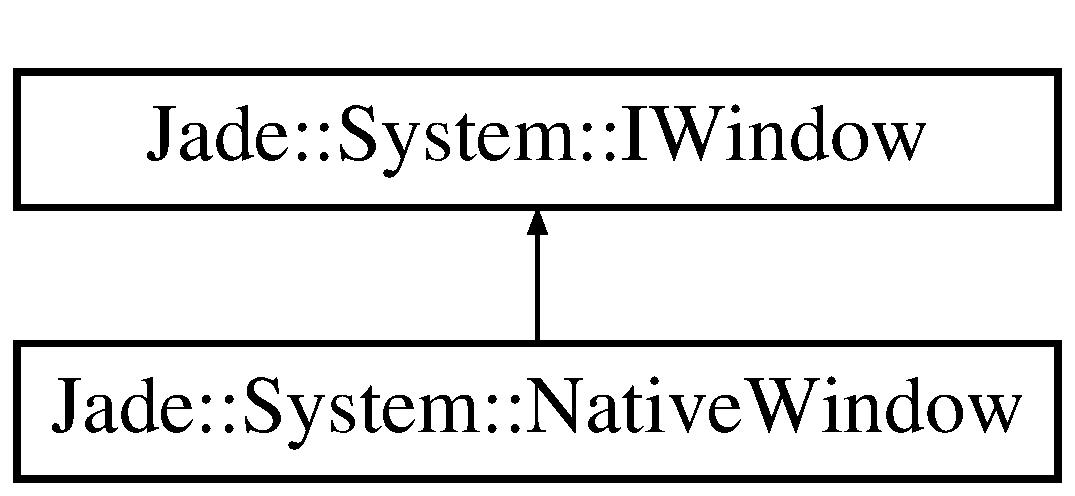
\includegraphics[height=2.000000cm]{class_jade_1_1_system_1_1_native_window}
\end{center}
\end{figure}
\subsection*{Public Member Functions}
\begin{DoxyCompactItemize}
\item 
\hypertarget{class_jade_1_1_system_1_1_native_window_a340e87c62e604ab931bb46e274a92fbb}{}int {\bfseries Get\+Width} () override\label{class_jade_1_1_system_1_1_native_window_a340e87c62e604ab931bb46e274a92fbb}

\item 
\hypertarget{class_jade_1_1_system_1_1_native_window_a16338fed3dede5a15e3ac3407980380a}{}void {\bfseries Set\+Width} (int value) override\label{class_jade_1_1_system_1_1_native_window_a16338fed3dede5a15e3ac3407980380a}

\item 
\hypertarget{class_jade_1_1_system_1_1_native_window_a37122bfb1149c77301dee67eec81e6ce}{}int {\bfseries Get\+Height} () override\label{class_jade_1_1_system_1_1_native_window_a37122bfb1149c77301dee67eec81e6ce}

\item 
\hypertarget{class_jade_1_1_system_1_1_native_window_a43808d2a6bdbfde47ef779b2a9f99f5b}{}void {\bfseries Set\+Height} (int value) override\label{class_jade_1_1_system_1_1_native_window_a43808d2a6bdbfde47ef779b2a9f99f5b}

\item 
\hypertarget{class_jade_1_1_system_1_1_native_window_a6c2c78580d13064c1846d4a5110c1a6e}{}float {\bfseries Get\+Aspect\+Ratio} () override\label{class_jade_1_1_system_1_1_native_window_a6c2c78580d13064c1846d4a5110c1a6e}

\item 
\hypertarget{class_jade_1_1_system_1_1_native_window_af20d2f3111fcdd2d331b0c7dad1202c8}{}int {\bfseries Get\+X} () override\label{class_jade_1_1_system_1_1_native_window_af20d2f3111fcdd2d331b0c7dad1202c8}

\item 
\hypertarget{class_jade_1_1_system_1_1_native_window_ac85f726a57868fde5b07c07fe3140b75}{}void {\bfseries Set\+X} (int value) override\label{class_jade_1_1_system_1_1_native_window_ac85f726a57868fde5b07c07fe3140b75}

\item 
\hypertarget{class_jade_1_1_system_1_1_native_window_ab83310067da365ffc0053bf99a7737dd}{}int {\bfseries Get\+Y} () override\label{class_jade_1_1_system_1_1_native_window_ab83310067da365ffc0053bf99a7737dd}

\item 
\hypertarget{class_jade_1_1_system_1_1_native_window_ab26ef2dcfab58d9334231190c076de6f}{}void {\bfseries Set\+Y} (int value) override\label{class_jade_1_1_system_1_1_native_window_ab26ef2dcfab58d9334231190c076de6f}

\item 
\hypertarget{class_jade_1_1_system_1_1_native_window_a21775d8b3abd191876b97c22eb2b90f1}{}std\+::string {\bfseries Get\+Title} () override\label{class_jade_1_1_system_1_1_native_window_a21775d8b3abd191876b97c22eb2b90f1}

\item 
\hypertarget{class_jade_1_1_system_1_1_native_window_a40e7d596064c2d2cc2f51268bd63883c}{}void {\bfseries Set\+Title} (std\+::string value) override\label{class_jade_1_1_system_1_1_native_window_a40e7d596064c2d2cc2f51268bd63883c}

\item 
\hypertarget{class_jade_1_1_system_1_1_native_window_ab7d6920378df512b2d37e1997efe2ed6}{}\hyperlink{class_jade_1_1_math_1_1_point}{Math\+::\+Point} {\bfseries Get\+Position} () override\label{class_jade_1_1_system_1_1_native_window_ab7d6920378df512b2d37e1997efe2ed6}

\item 
\hypertarget{class_jade_1_1_system_1_1_native_window_af36a9bdd4c95a8fc2a05ac0aadd7650e}{}void {\bfseries Set\+Position} (int x, int y) override\label{class_jade_1_1_system_1_1_native_window_af36a9bdd4c95a8fc2a05ac0aadd7650e}

\item 
\hypertarget{class_jade_1_1_system_1_1_native_window_a2452bbf1e7ee28815add632fd05e9399}{}void {\bfseries Set\+Icon} (std\+::string filename) override\label{class_jade_1_1_system_1_1_native_window_a2452bbf1e7ee28815add632fd05e9399}

\item 
\hypertarget{class_jade_1_1_system_1_1_native_window_ad7cdd6d0f1e0a237a74a146b4f51e86d}{}void {\bfseries Close} () override\label{class_jade_1_1_system_1_1_native_window_ad7cdd6d0f1e0a237a74a146b4f51e86d}

\item 
\hypertarget{class_jade_1_1_system_1_1_native_window_a4e78af761ee6598512769faada4edbab}{}void $\ast$ {\bfseries Handle} () override\label{class_jade_1_1_system_1_1_native_window_a4e78af761ee6598512769faada4edbab}

\item 
\hypertarget{class_jade_1_1_system_1_1_native_window_a2528e5b7365c4699f60a1069e9f6f71f}{}void {\bfseries Show} () override\label{class_jade_1_1_system_1_1_native_window_a2528e5b7365c4699f60a1069e9f6f71f}

\item 
\hypertarget{class_jade_1_1_system_1_1_native_window_a62ba6c4a598ab86db4fd9d684fc83d5c}{}void {\bfseries Hide} () override\label{class_jade_1_1_system_1_1_native_window_a62ba6c4a598ab86db4fd9d684fc83d5c}

\item 
\hypertarget{class_jade_1_1_system_1_1_native_window_a6ad5a215e71e19fdd1c95de27626843f}{}void {\bfseries Restore} () override\label{class_jade_1_1_system_1_1_native_window_a6ad5a215e71e19fdd1c95de27626843f}

\item 
\hypertarget{class_jade_1_1_system_1_1_native_window_aa761d97a973e42042c947a1464ea77a1}{}void {\bfseries Maximize} () override\label{class_jade_1_1_system_1_1_native_window_aa761d97a973e42042c947a1464ea77a1}

\item 
\hypertarget{class_jade_1_1_system_1_1_native_window_aad29faecc2038b6c41320bf41be21004}{}bool {\bfseries Is\+Minimized} () override\label{class_jade_1_1_system_1_1_native_window_aad29faecc2038b6c41320bf41be21004}

\item 
\hypertarget{class_jade_1_1_system_1_1_native_window_a2efbd7057d5614d57a1eb7dfe852b5b2}{}void {\bfseries Minimize} () override\label{class_jade_1_1_system_1_1_native_window_a2efbd7057d5614d57a1eb7dfe852b5b2}

\item 
\hypertarget{class_jade_1_1_system_1_1_native_window_a2f5dc616023406c2ad2f0114feeca3f8}{}bool {\bfseries Is\+Maximized} () override\label{class_jade_1_1_system_1_1_native_window_a2f5dc616023406c2ad2f0114feeca3f8}

\item 
\hypertarget{class_jade_1_1_system_1_1_native_window_a31b73c3253d99fad80d017701882af7e}{}bool {\bfseries Is\+Visible} () override\label{class_jade_1_1_system_1_1_native_window_a31b73c3253d99fad80d017701882af7e}

\item 
\hypertarget{class_jade_1_1_system_1_1_native_window_a49af1c9967504f90f5bea8a6b58090f6}{}bool {\bfseries Is\+Open} () override\label{class_jade_1_1_system_1_1_native_window_a49af1c9967504f90f5bea8a6b58090f6}

\item 
\hypertarget{class_jade_1_1_system_1_1_native_window_a2ee0c135f10b384ed3a9dc5a53ec2c16}{}bool {\bfseries Is\+Fullscreen} () override\label{class_jade_1_1_system_1_1_native_window_a2ee0c135f10b384ed3a9dc5a53ec2c16}

\item 
\hypertarget{class_jade_1_1_system_1_1_native_window_a599df3a529a57565c3608af5d17a7aa0}{}bool {\bfseries Is\+Active} () override\label{class_jade_1_1_system_1_1_native_window_a599df3a529a57565c3608af5d17a7aa0}

\item 
\hypertarget{class_jade_1_1_system_1_1_native_window_aa759a2e68dfc0f39be2e508866fcdf28}{}\hyperlink{class_jade_1_1_system_1_1_timer}{System\+::\+Timer} {\bfseries Get\+Timer} () override\label{class_jade_1_1_system_1_1_native_window_aa759a2e68dfc0f39be2e508866fcdf28}

\item 
\hypertarget{class_jade_1_1_system_1_1_native_window_ac36d165a709f1fddce8c4408188b45d1}{}\hyperlink{struct_jade_1_1_input_1_1_input}{Input\+::\+Input} {\bfseries Get\+Input} () override\label{class_jade_1_1_system_1_1_native_window_ac36d165a709f1fddce8c4408188b45d1}

\item 
\hypertarget{class_jade_1_1_system_1_1_native_window_a5798bbff6f1d6dd8c0ada281b93de7a5}{}{\bfseries Native\+Window} (int width, int height, int x, int y, std\+::string title, bool fullscreen)\label{class_jade_1_1_system_1_1_native_window_a5798bbff6f1d6dd8c0ada281b93de7a5}

\end{DoxyCompactItemize}


The documentation for this class was generated from the following files\+:\begin{DoxyCompactItemize}
\item 
C\+:/\+Users/\+Ben/\+Documents/\+Git\+Hub/\+Jade/\+Jade/\+Source/\+System/\+Window/Native\+Window.\+h\item 
C\+:/\+Users/\+Ben/\+Documents/\+Git\+Hub/\+Jade/\+Jade/\+Source/\+System/\+Window/Native\+Window.\+cpp\end{DoxyCompactItemize}

\hypertarget{struct_jade_1_1_math_1_1_never_changes}{}\section{Jade\+:\+:Math\+:\+:Never\+Changes Struct Reference}
\label{struct_jade_1_1_math_1_1_never_changes}\index{Jade\+::\+Math\+::\+Never\+Changes@{Jade\+::\+Math\+::\+Never\+Changes}}
\subsection*{Public Attributes}
\begin{DoxyCompactItemize}
\item 
\hypertarget{struct_jade_1_1_math_1_1_never_changes_a5908973be46b89c468e79e58970a15f0}{}\hyperlink{struct_jade_1_1_math_1_1_matrix}{Matrix} {\bfseries view}\label{struct_jade_1_1_math_1_1_never_changes_a5908973be46b89c468e79e58970a15f0}

\end{DoxyCompactItemize}


The documentation for this struct was generated from the following file\+:\begin{DoxyCompactItemize}
\item 
C\+:/\+Users/\+Ben/\+Documents/\+Git\+Hub/\+Jade/\+Jade/\+Source/\+Math/Space.\+h\end{DoxyCompactItemize}

\hypertarget{struct_jade_1_1_math_1_1_on_resize}{}\section{Jade\+:\+:Math\+:\+:On\+Resize Struct Reference}
\label{struct_jade_1_1_math_1_1_on_resize}\index{Jade\+::\+Math\+::\+On\+Resize@{Jade\+::\+Math\+::\+On\+Resize}}
\subsection*{Public Attributes}
\begin{DoxyCompactItemize}
\item 
\hypertarget{struct_jade_1_1_math_1_1_on_resize_ae4073cea394b68822c6a707fd4ae1afe}{}\hyperlink{struct_jade_1_1_math_1_1_matrix}{Matrix} {\bfseries projection}\label{struct_jade_1_1_math_1_1_on_resize_ae4073cea394b68822c6a707fd4ae1afe}

\end{DoxyCompactItemize}


The documentation for this struct was generated from the following file\+:\begin{DoxyCompactItemize}
\item 
C\+:/\+Users/\+Ben/\+Documents/\+Git\+Hub/\+Jade/\+Jade/\+Source/\+Math/Space.\+h\end{DoxyCompactItemize}

\hypertarget{struct_jade_1_1_math_1_1_per_object}{}\section{Jade\+:\+:Math\+:\+:Per\+Object Struct Reference}
\label{struct_jade_1_1_math_1_1_per_object}\index{Jade\+::\+Math\+::\+Per\+Object@{Jade\+::\+Math\+::\+Per\+Object}}
\subsection*{Public Attributes}
\begin{DoxyCompactItemize}
\item 
\hypertarget{struct_jade_1_1_math_1_1_per_object_ab6e1f936ada0c7d91e330a6a1f102083}{}\hyperlink{struct_jade_1_1_math_1_1_matrix}{Matrix} {\bfseries world}\label{struct_jade_1_1_math_1_1_per_object_ab6e1f936ada0c7d91e330a6a1f102083}

\end{DoxyCompactItemize}


The documentation for this struct was generated from the following file\+:\begin{DoxyCompactItemize}
\item 
C\+:/\+Users/\+Ben/\+Documents/\+Git\+Hub/\+Jade/\+Jade/\+Source/\+Math/Space.\+h\end{DoxyCompactItemize}

\hypertarget{class_jade_1_1_system_1_1_platform}{}\section{Jade\+:\+:System\+:\+:Platform Class Reference}
\label{class_jade_1_1_system_1_1_platform}\index{Jade\+::\+System\+::\+Platform@{Jade\+::\+System\+::\+Platform}}
\subsection*{Public Types}
\begin{DoxyCompactItemize}
\item 
\hypertarget{class_jade_1_1_system_1_1_platform_a863c143f8bd803f8d76bf31965681b4b}{}enum {\bfseries Platform\+I\+D} \+: int \{ {\bfseries Unknown} = 0, 
{\bfseries Windows} = 1, 
{\bfseries Mac\+O\+S\+X} = 2, 
{\bfseries Linux} = 3
 \}\label{class_jade_1_1_system_1_1_platform_a863c143f8bd803f8d76bf31965681b4b}

\end{DoxyCompactItemize}
\subsection*{Static Public Member Functions}
\begin{DoxyCompactItemize}
\item 
\hypertarget{class_jade_1_1_system_1_1_platform_adf4687dad2e5c57f03c52d95518f683a}{}static Platform\+I\+D {\bfseries Get\+Platform\+I\+D} ()\label{class_jade_1_1_system_1_1_platform_adf4687dad2e5c57f03c52d95518f683a}

\end{DoxyCompactItemize}


The documentation for this class was generated from the following file\+:\begin{DoxyCompactItemize}
\item 
C\+:/\+Users/\+Ben/\+Documents/\+Git\+Hub/\+Jade/\+Jade/\+Source/\+System/Platform.\+h\end{DoxyCompactItemize}

\hypertarget{class_jade_1_1_math_1_1_point}{}\section{Jade\+:\+:Math\+:\+:Point Class Reference}
\label{class_jade_1_1_math_1_1_point}\index{Jade\+::\+Math\+::\+Point@{Jade\+::\+Math\+::\+Point}}
\subsection*{Public Member Functions}
\begin{DoxyCompactItemize}
\item 
\hypertarget{class_jade_1_1_math_1_1_point_af7fb5d8ba845c62043aa8c1147dab365}{}{\bfseries Point} (float x, float y)\label{class_jade_1_1_math_1_1_point_af7fb5d8ba845c62043aa8c1147dab365}

\end{DoxyCompactItemize}


The documentation for this class was generated from the following file\+:\begin{DoxyCompactItemize}
\item 
C\+:/\+Users/\+Ben/\+Documents/\+Git\+Hub/\+Jade/\+Jade/\+Source/\+Math/Point.\+h\end{DoxyCompactItemize}

\hypertarget{struct_jade_1_1_math_1_1_quaternion}{}\section{Jade\+:\+:Math\+:\+:Quaternion Struct Reference}
\label{struct_jade_1_1_math_1_1_quaternion}\index{Jade\+::\+Math\+::\+Quaternion@{Jade\+::\+Math\+::\+Quaternion}}


The documentation for this struct was generated from the following file\+:\begin{DoxyCompactItemize}
\item 
C\+:/\+Users/\+Ben/\+Documents/\+Git\+Hub/\+Jade/\+Jade/\+Source/\+Math/Quaternion.\+h\end{DoxyCompactItemize}

\hypertarget{class_jade_1_1_graphics_1_1_rasterizer}{}\section{Jade\+:\+:Graphics\+:\+:Rasterizer Class Reference}
\label{class_jade_1_1_graphics_1_1_rasterizer}\index{Jade\+::\+Graphics\+::\+Rasterizer@{Jade\+::\+Graphics\+::\+Rasterizer}}
\subsection*{Public Member Functions}
\begin{DoxyCompactItemize}
\item 
\hypertarget{class_jade_1_1_graphics_1_1_rasterizer_a4aa26ad8f6501e4adfcde35d351fc176}{}{\bfseries Rasterizer} (\hyperlink{class_jade_1_1_graphics_1_1_device}{Device} device)\label{class_jade_1_1_graphics_1_1_rasterizer_a4aa26ad8f6501e4adfcde35d351fc176}

\item 
bool \hyperlink{class_jade_1_1_graphics_1_1_rasterizer_aa4dfe961881a063f3e7e0b3e2a03500a}{Set\+Rasterizer\+State} (Cull\+Mode cull\+Mode, Fill\+Mode fill\+Mode, Wind\+Mode wind\+Mode) const 
\begin{DoxyCompactList}\small\item\em Sets the rasterizer state to the specified cull and fill mode. \end{DoxyCompactList}\item 
\hypertarget{class_jade_1_1_graphics_1_1_rasterizer_a6b64516bb21e19638f6e9b1d5d600d97}{}Cull\+Mode \hyperlink{class_jade_1_1_graphics_1_1_rasterizer_a6b64516bb21e19638f6e9b1d5d600d97}{Get\+Cull\+Mode} () const \label{class_jade_1_1_graphics_1_1_rasterizer_a6b64516bb21e19638f6e9b1d5d600d97}

\begin{DoxyCompactList}\small\item\em Returns the current cull mode. Return values can only be None, Front, or Back. \end{DoxyCompactList}\item 
\hypertarget{class_jade_1_1_graphics_1_1_rasterizer_aec61b803aa6bb26e9f7002eca858e1b6}{}Fill\+Mode \hyperlink{class_jade_1_1_graphics_1_1_rasterizer_aec61b803aa6bb26e9f7002eca858e1b6}{Get\+Fill\+Mode} () const \label{class_jade_1_1_graphics_1_1_rasterizer_aec61b803aa6bb26e9f7002eca858e1b6}

\begin{DoxyCompactList}\small\item\em Returns the current fill mode. Return values can only be Wireframe or Solid. \end{DoxyCompactList}\item 
\hypertarget{class_jade_1_1_graphics_1_1_rasterizer_a67934284de71de2de67a6183fcb94734}{}Wind\+Mode \hyperlink{class_jade_1_1_graphics_1_1_rasterizer_a67934284de71de2de67a6183fcb94734}{Get\+Wind\+Mode} () const \label{class_jade_1_1_graphics_1_1_rasterizer_a67934284de71de2de67a6183fcb94734}

\begin{DoxyCompactList}\small\item\em Returns the current wind mode. Return value can only be Clockwise or Counter\+Clockwise. \end{DoxyCompactList}\end{DoxyCompactItemize}


\subsection{Member Function Documentation}
\hypertarget{class_jade_1_1_graphics_1_1_rasterizer_aa4dfe961881a063f3e7e0b3e2a03500a}{}\index{Jade\+::\+Graphics\+::\+Rasterizer@{Jade\+::\+Graphics\+::\+Rasterizer}!Set\+Rasterizer\+State@{Set\+Rasterizer\+State}}
\index{Set\+Rasterizer\+State@{Set\+Rasterizer\+State}!Jade\+::\+Graphics\+::\+Rasterizer@{Jade\+::\+Graphics\+::\+Rasterizer}}
\subsubsection[{Set\+Rasterizer\+State(\+Cull\+Mode cull\+Mode, Fill\+Mode fill\+Mode, Wind\+Mode wind\+Mode) const }]{\setlength{\rightskip}{0pt plus 5cm}bool Jade\+::\+Graphics\+::\+Rasterizer\+::\+Set\+Rasterizer\+State (
\begin{DoxyParamCaption}
\item[{Cull\+Mode}]{cull\+Mode, }
\item[{Fill\+Mode}]{fill\+Mode, }
\item[{Wind\+Mode}]{wind\+Mode}
\end{DoxyParamCaption}
) const\hspace{0.3cm}{\ttfamily [inline]}}\label{class_jade_1_1_graphics_1_1_rasterizer_aa4dfe961881a063f3e7e0b3e2a03500a}


Sets the rasterizer state to the specified cull and fill mode. 


\begin{DoxyParams}[1]{Parameters}
\mbox{\tt in}  & {\em cull\+Mode} & Represents the faces that will be hidden from view when rendering. Front, Back, and None are accepted values here. \\
\hline
\mbox{\tt in}  & {\em fill\+Mode} & Represents how the faces will be rendered. Solid and Wireframe are accepted values here. \\
\hline
\end{DoxyParams}


The documentation for this class was generated from the following file\+:\begin{DoxyCompactItemize}
\item 
C\+:/\+Users/\+Ben/\+Documents/\+Git\+Hub/\+Jade/\+Jade/\+Source/\+Graphics/\+Rasterizer/Rasterizer.\+h\end{DoxyCompactItemize}

\hypertarget{class_jade_1_1_graphics_1_1_rasterizer_factory}{}\section{Jade\+:\+:Graphics\+:\+:Rasterizer\+Factory Class Reference}
\label{class_jade_1_1_graphics_1_1_rasterizer_factory}\index{Jade\+::\+Graphics\+::\+Rasterizer\+Factory@{Jade\+::\+Graphics\+::\+Rasterizer\+Factory}}
\subsection*{Static Public Member Functions}
\begin{DoxyCompactItemize}
\item 
\hypertarget{class_jade_1_1_graphics_1_1_rasterizer_factory_ab9d99dc1f3e7dabfb08cd6497efb8484}{}{\footnotesize template$<$typename T $>$ }\\static std\+::shared\+\_\+ptr$<$ T $>$ {\bfseries Generate} (\hyperlink{class_jade_1_1_graphics_1_1_device}{Device} device)\label{class_jade_1_1_graphics_1_1_rasterizer_factory_ab9d99dc1f3e7dabfb08cd6497efb8484}

\end{DoxyCompactItemize}


The documentation for this class was generated from the following file\+:\begin{DoxyCompactItemize}
\item 
C\+:/\+Users/\+Ben/\+Documents/\+Git\+Hub/\+Jade/\+Jade/\+Source/\+Graphics/\+Rasterizer/Rasterizer\+Factory.\+h\end{DoxyCompactItemize}

\hypertarget{class_jade_1_1_math_1_1_ray}{}\section{Jade\+:\+:Math\+:\+:Ray Class Reference}
\label{class_jade_1_1_math_1_1_ray}\index{Jade\+::\+Math\+::\+Ray@{Jade\+::\+Math\+::\+Ray}}


The documentation for this class was generated from the following file\+:\begin{DoxyCompactItemize}
\item 
C\+:/\+Users/\+Ben/\+Documents/\+Git\+Hub/\+Jade/\+Jade/\+Source/\+Math/Ray.\+h\end{DoxyCompactItemize}

\hypertarget{class_jade_1_1_math_1_1_rectangle}{}\section{Jade\+:\+:Math\+:\+:Rectangle Class Reference}
\label{class_jade_1_1_math_1_1_rectangle}\index{Jade\+::\+Math\+::\+Rectangle@{Jade\+::\+Math\+::\+Rectangle}}
\subsection*{Public Member Functions}
\begin{DoxyCompactItemize}
\item 
\hypertarget{class_jade_1_1_math_1_1_rectangle_a81b43b9a6c1700fdb71fb42f6a18ae18}{}{\bfseries Rectangle} (float x, float y, float width, float height)\label{class_jade_1_1_math_1_1_rectangle_a81b43b9a6c1700fdb71fb42f6a18ae18}

\end{DoxyCompactItemize}


The documentation for this class was generated from the following file\+:\begin{DoxyCompactItemize}
\item 
C\+:/\+Users/\+Ben/\+Documents/\+Git\+Hub/\+Jade/\+Jade/\+Source/\+Math/Rectangle.\+h\end{DoxyCompactItemize}

\hypertarget{class_jade_1_1_graphics_1_1_script}{}\section{Jade\+:\+:Graphics\+:\+:Script Class Reference}
\label{class_jade_1_1_graphics_1_1_script}\index{Jade\+::\+Graphics\+::\+Script@{Jade\+::\+Graphics\+::\+Script}}


The documentation for this class was generated from the following file\+:\begin{DoxyCompactItemize}
\item 
C\+:/\+Users/\+Ben/\+Documents/\+Git\+Hub/\+Jade/\+Jade/\+Source/\+Core/\+Script/Script.\+h\end{DoxyCompactItemize}

\hypertarget{class_jade_1_1_graphics_1_1_shader}{}\section{Jade\+:\+:Graphics\+:\+:Shader Class Reference}
\label{class_jade_1_1_graphics_1_1_shader}\index{Jade\+::\+Graphics\+::\+Shader@{Jade\+::\+Graphics\+::\+Shader}}
\subsection*{Public Member Functions}
\begin{DoxyCompactItemize}
\item 
\hypertarget{class_jade_1_1_graphics_1_1_shader_a6ba8cfe295f29771b8b56590ff39181b}{}{\bfseries Shader} (\hyperlink{class_jade_1_1_graphics_1_1_device}{Device} device, std\+::map$<$ std\+::string, Shader\+Type $>$ shaders)\label{class_jade_1_1_graphics_1_1_shader_a6ba8cfe295f29771b8b56590ff39181b}

\end{DoxyCompactItemize}


The documentation for this class was generated from the following files\+:\begin{DoxyCompactItemize}
\item 
C\+:/\+Users/\+Ben/\+Documents/\+Git\+Hub/\+Jade/\+Jade/\+Source/\+Graphics/\+Shader/Shader.\+h\item 
C\+:/\+Users/\+Ben/\+Documents/\+Git\+Hub/\+Jade/\+Jade/\+Source/\+Graphics/\+Shader/Shader.\+cpp\end{DoxyCompactItemize}

\hypertarget{class_jade_1_1_core_1_1_shader_creation_exception}{}\section{Jade\+:\+:Core\+:\+:Shader\+Creation\+Exception Class Reference}
\label{class_jade_1_1_core_1_1_shader_creation_exception}\index{Jade\+::\+Core\+::\+Shader\+Creation\+Exception@{Jade\+::\+Core\+::\+Shader\+Creation\+Exception}}
Inheritance diagram for Jade\+:\+:Core\+:\+:Shader\+Creation\+Exception\+:\begin{figure}[H]
\begin{center}
\leavevmode
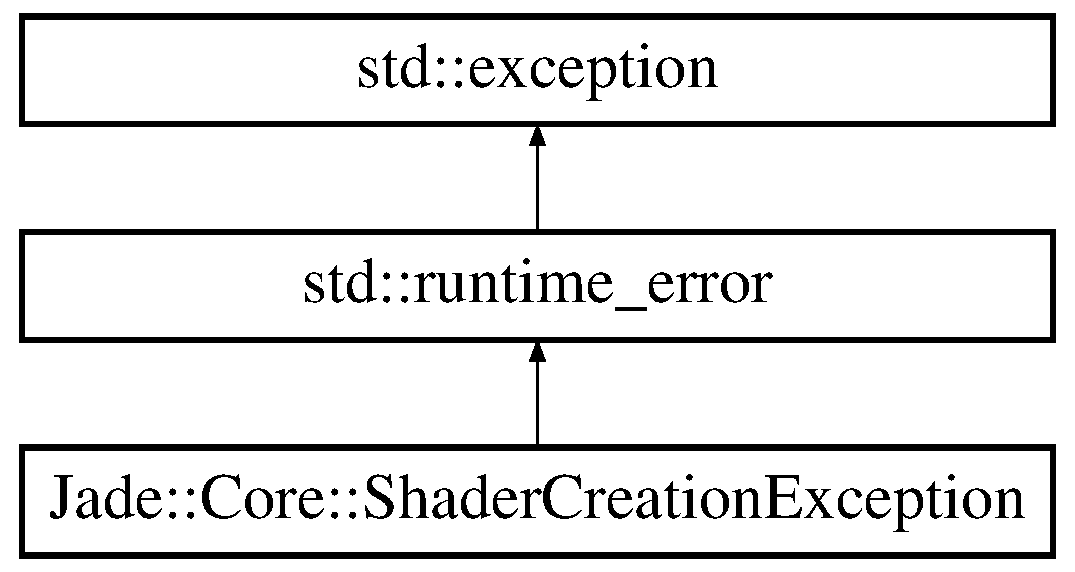
\includegraphics[height=3.000000cm]{class_jade_1_1_core_1_1_shader_creation_exception}
\end{center}
\end{figure}


The documentation for this class was generated from the following file\+:\begin{DoxyCompactItemize}
\item 
C\+:/\+Users/\+Ben/\+Documents/\+Git\+Hub/\+Jade/\+Jade/\+Source/\+Core/\+Exception/Shader\+Creation\+Exception.\+h\end{DoxyCompactItemize}

\hypertarget{struct_jade_1_1_graphics_1_1_specification}{}\section{Jade\+:\+:Graphics\+:\+:Specification Struct Reference}
\label{struct_jade_1_1_graphics_1_1_specification}\index{Jade\+::\+Graphics\+::\+Specification@{Jade\+::\+Graphics\+::\+Specification}}
\subsection*{Public Attributes}
\begin{DoxyCompactItemize}
\item 
\hypertarget{struct_jade_1_1_graphics_1_1_specification_a76947e56f89284a056142d36549925d1}{}int {\bfseries back\+Buffer\+Width}\label{struct_jade_1_1_graphics_1_1_specification_a76947e56f89284a056142d36549925d1}

\item 
\hypertarget{struct_jade_1_1_graphics_1_1_specification_af66492f2015f718021e8a43a389bfb53}{}int {\bfseries back\+Buffer\+Height}\label{struct_jade_1_1_graphics_1_1_specification_af66492f2015f718021e8a43a389bfb53}

\item 
\hypertarget{struct_jade_1_1_graphics_1_1_specification_a7c86964edc5f3923a7658b561f4d6bb4}{}int {\bfseries color\+Bits}\label{struct_jade_1_1_graphics_1_1_specification_a7c86964edc5f3923a7658b561f4d6bb4}

\item 
\hypertarget{struct_jade_1_1_graphics_1_1_specification_ad941863bb47f1069f04afe226d1007d0}{}int {\bfseries samples}\label{struct_jade_1_1_graphics_1_1_specification_ad941863bb47f1069f04afe226d1007d0}

\item 
\hypertarget{struct_jade_1_1_graphics_1_1_specification_ab1c4c9ce465199a05169cb9404b76811}{}bool {\bfseries vsync}\label{struct_jade_1_1_graphics_1_1_specification_ab1c4c9ce465199a05169cb9404b76811}

\end{DoxyCompactItemize}


The documentation for this struct was generated from the following file\+:\begin{DoxyCompactItemize}
\item 
C\+:/\+Users/\+Ben/\+Documents/\+Git\+Hub/\+Jade/\+Jade/\+Source/\+Graphics/\+Device/Specification.\+h\end{DoxyCompactItemize}

\hypertarget{class_jade_1_1_graphics_1_1_texture}{}\section{Jade\+:\+:Graphics\+:\+:Texture Class Reference}
\label{class_jade_1_1_graphics_1_1_texture}\index{Jade\+::\+Graphics\+::\+Texture@{Jade\+::\+Graphics\+::\+Texture}}
\subsection*{Public Member Functions}
\begin{DoxyCompactItemize}
\item 
\hypertarget{class_jade_1_1_graphics_1_1_texture_a59de955b57a5db4845792cef4c9959d9}{}{\bfseries Texture} (\hyperlink{class_jade_1_1_graphics_1_1_device}{Device} device, std\+::string filename, Texture\+Type type)\label{class_jade_1_1_graphics_1_1_texture_a59de955b57a5db4845792cef4c9959d9}

\item 
\hypertarget{class_jade_1_1_graphics_1_1_texture_aba04918ff5aff35169ebfe6fdeac6727}{}bool {\bfseries Create\+Texture\+From\+File} () const \label{class_jade_1_1_graphics_1_1_texture_aba04918ff5aff35169ebfe6fdeac6727}

\item 
\hypertarget{class_jade_1_1_graphics_1_1_texture_a5330c4e0ace59056884388cf8be3c9ee}{}std\+::string {\bfseries Get\+Filename} ()\label{class_jade_1_1_graphics_1_1_texture_a5330c4e0ace59056884388cf8be3c9ee}

\item 
\hypertarget{class_jade_1_1_graphics_1_1_texture_accc5f797f7d2f9cf4c2b4f3b65dc8839}{}std\+::shared\+\_\+ptr$<$ \hyperlink{struct_jade_1_1_graphics_1_1_i_texture}{I\+Texture} $>$ {\bfseries Get\+I\+Texture} () const \label{class_jade_1_1_graphics_1_1_texture_accc5f797f7d2f9cf4c2b4f3b65dc8839}

\end{DoxyCompactItemize}


The documentation for this class was generated from the following file\+:\begin{DoxyCompactItemize}
\item 
C\+:/\+Users/\+Ben/\+Documents/\+Git\+Hub/\+Jade/\+Jade/\+Source/\+Graphics/\+Texture/Texture.\+h\end{DoxyCompactItemize}

\hypertarget{class_jade_1_1_graphics_1_1_texture_factory}{}\section{Jade\+:\+:Graphics\+:\+:Texture\+Factory Class Reference}
\label{class_jade_1_1_graphics_1_1_texture_factory}\index{Jade\+::\+Graphics\+::\+Texture\+Factory@{Jade\+::\+Graphics\+::\+Texture\+Factory}}
\subsection*{Static Public Member Functions}
\begin{DoxyCompactItemize}
\item 
\hypertarget{class_jade_1_1_graphics_1_1_texture_factory_a378568ba62fa85bb98fd76d625f1fd0b}{}{\footnotesize template$<$typename T , typename... Params$>$ }\\static std\+::shared\+\_\+ptr$<$ T $>$ {\bfseries Generate} (\hyperlink{class_jade_1_1_graphics_1_1_device}{Device} device, Params...\+params)\label{class_jade_1_1_graphics_1_1_texture_factory_a378568ba62fa85bb98fd76d625f1fd0b}

\end{DoxyCompactItemize}


The documentation for this class was generated from the following file\+:\begin{DoxyCompactItemize}
\item 
C\+:/\+Users/\+Ben/\+Documents/\+Git\+Hub/\+Jade/\+Jade/\+Source/\+Graphics/\+Texture/Texture\+Factory.\+h\end{DoxyCompactItemize}

\hypertarget{class_jade_1_1_system_1_1_thread}{}\section{Jade\+:\+:System\+:\+:Thread Class Reference}
\label{class_jade_1_1_system_1_1_thread}\index{Jade\+::\+System\+::\+Thread@{Jade\+::\+System\+::\+Thread}}
\subsection*{Public Member Functions}
\begin{DoxyCompactItemize}
\item 
\hypertarget{class_jade_1_1_system_1_1_thread_a192fdadcd198c2d6110906fbdd56f92a}{}void {\bfseries Execute} (std\+::thread thread)\label{class_jade_1_1_system_1_1_thread_a192fdadcd198c2d6110906fbdd56f92a}

\end{DoxyCompactItemize}


The documentation for this class was generated from the following files\+:\begin{DoxyCompactItemize}
\item 
C\+:/\+Users/\+Ben/\+Documents/\+Git\+Hub/\+Jade/\+Jade/\+Source/\+System/Thread.\+h\item 
C\+:/\+Users/\+Ben/\+Documents/\+Git\+Hub/\+Jade/\+Jade/\+Source/\+System/Thread.\+cpp\end{DoxyCompactItemize}

\hypertarget{class_jade_1_1_system_1_1_timer}{}\section{Jade\+:\+:System\+:\+:Timer Class Reference}
\label{class_jade_1_1_system_1_1_timer}\index{Jade\+::\+System\+::\+Timer@{Jade\+::\+System\+::\+Timer}}
\subsection*{Public Member Functions}
\begin{DoxyCompactItemize}
\item 
\hypertarget{class_jade_1_1_system_1_1_timer_a98d6cf8fcc1b9402f327c048159423c9}{}float {\bfseries Get\+Delta\+Time} () const \label{class_jade_1_1_system_1_1_timer_a98d6cf8fcc1b9402f327c048159423c9}

\item 
\hypertarget{class_jade_1_1_system_1_1_timer_a6ecf21b869b1890514dc6b68b119a6c7}{}void {\bfseries Set\+Delta\+Time} (float value)\label{class_jade_1_1_system_1_1_timer_a6ecf21b869b1890514dc6b68b119a6c7}

\item 
\hypertarget{class_jade_1_1_system_1_1_timer_a8ded659a510f3bb3f5e1b7132bb7eeb2}{}float {\bfseries Get\+Elasped\+Time} () const \label{class_jade_1_1_system_1_1_timer_a8ded659a510f3bb3f5e1b7132bb7eeb2}

\item 
\hypertarget{class_jade_1_1_system_1_1_timer_abd0304fb7ec5b84cb1c6e1eed127387b}{}void {\bfseries Set\+Elapsed\+Time} (float value)\label{class_jade_1_1_system_1_1_timer_abd0304fb7ec5b84cb1c6e1eed127387b}

\end{DoxyCompactItemize}


The documentation for this class was generated from the following file\+:\begin{DoxyCompactItemize}
\item 
C\+:/\+Users/\+Ben/\+Documents/\+Git\+Hub/\+Jade/\+Jade/\+Source/\+System/Timer.\+h\end{DoxyCompactItemize}

\hypertarget{class_jade_1_1_core_1_1_utility}{}\section{Jade\+:\+:Core\+:\+:Utility Class Reference}
\label{class_jade_1_1_core_1_1_utility}\index{Jade\+::\+Core\+::\+Utility@{Jade\+::\+Core\+::\+Utility}}
\subsection*{Static Public Member Functions}
\begin{DoxyCompactItemize}
\item 
\hypertarget{class_jade_1_1_core_1_1_utility_a5c3cc38dda87f98c783a0229071b352a}{}static std\+::string {\bfseries Get\+File\+Path} ()\label{class_jade_1_1_core_1_1_utility_a5c3cc38dda87f98c783a0229071b352a}

\item 
\hypertarget{class_jade_1_1_core_1_1_utility_ae01de942236cb4bb6067ea55d1e5eaa5}{}static std\+::wstring {\bfseries String\+To\+W\+String} (std\+::string string)\label{class_jade_1_1_core_1_1_utility_ae01de942236cb4bb6067ea55d1e5eaa5}

\end{DoxyCompactItemize}


The documentation for this class was generated from the following files\+:\begin{DoxyCompactItemize}
\item 
C\+:/\+Users/\+Ben/\+Documents/\+Git\+Hub/\+Jade/\+Jade/\+Source/\+Core/Utility.\+h\item 
C\+:/\+Users/\+Ben/\+Documents/\+Git\+Hub/\+Jade/\+Jade/\+Source/\+Core/Utility.\+cpp\end{DoxyCompactItemize}

\hypertarget{struct_jade_1_1_math_1_1_vector2}{}\section{Jade\+:\+:Math\+:\+:Vector2 Struct Reference}
\label{struct_jade_1_1_math_1_1_vector2}\index{Jade\+::\+Math\+::\+Vector2@{Jade\+::\+Math\+::\+Vector2}}
\subsection*{Public Member Functions}
\begin{DoxyCompactItemize}
\item 
\hypertarget{struct_jade_1_1_math_1_1_vector2_a7c927668c9cf1bcb510b97f505e9ff1c}{}bool {\bfseries operator==} (const \hyperlink{struct_jade_1_1_math_1_1_vector2}{Vector2} vector)\label{struct_jade_1_1_math_1_1_vector2_a7c927668c9cf1bcb510b97f505e9ff1c}

\item 
\hypertarget{struct_jade_1_1_math_1_1_vector2_a3184e930d7610c445449eacc26e6ecd3}{}bool {\bfseries operator!=} (const \hyperlink{struct_jade_1_1_math_1_1_vector2}{Vector2} vector)\label{struct_jade_1_1_math_1_1_vector2_a3184e930d7610c445449eacc26e6ecd3}

\item 
\hypertarget{struct_jade_1_1_math_1_1_vector2_a62707e92121bba9df43225ab1c920702}{}\hyperlink{struct_jade_1_1_math_1_1_vector2}{Vector2} {\bfseries operator+} (const \hyperlink{struct_jade_1_1_math_1_1_vector2}{Vector2} vector)\label{struct_jade_1_1_math_1_1_vector2_a62707e92121bba9df43225ab1c920702}

\item 
\hypertarget{struct_jade_1_1_math_1_1_vector2_aae78ed21c27a88486cdd39345e732826}{}\hyperlink{struct_jade_1_1_math_1_1_vector2}{Vector2} {\bfseries operator-\/} (const \hyperlink{struct_jade_1_1_math_1_1_vector2}{Vector2} vector)\label{struct_jade_1_1_math_1_1_vector2_aae78ed21c27a88486cdd39345e732826}

\item 
\hypertarget{struct_jade_1_1_math_1_1_vector2_abd744dd74a1259811db2ed0fab7546f0}{}\hyperlink{struct_jade_1_1_math_1_1_vector2}{Vector2} {\bfseries operator$\ast$} (const float scalar)\label{struct_jade_1_1_math_1_1_vector2_abd744dd74a1259811db2ed0fab7546f0}

\item 
\hypertarget{struct_jade_1_1_math_1_1_vector2_a8988aff2f26ae306413ccd0c0381f0a4}{}\hyperlink{struct_jade_1_1_math_1_1_vector2}{Vector2} {\bfseries operator/} (const float scalar)\label{struct_jade_1_1_math_1_1_vector2_a8988aff2f26ae306413ccd0c0381f0a4}

\item 
\hypertarget{struct_jade_1_1_math_1_1_vector2_ab320239a30e8576e6a644ddfb269b40f}{}{\bfseries Vector2} (float x, float y)\label{struct_jade_1_1_math_1_1_vector2_ab320239a30e8576e6a644ddfb269b40f}

\item 
\hypertarget{struct_jade_1_1_math_1_1_vector2_ac196020f2a95b05cd511dfab3e0385ba}{}float {\bfseries Distance} (\hyperlink{struct_jade_1_1_math_1_1_vector2}{Vector2} target)\label{struct_jade_1_1_math_1_1_vector2_ac196020f2a95b05cd511dfab3e0385ba}

\item 
\hypertarget{struct_jade_1_1_math_1_1_vector2_a42da30ca3cd936c99f3e31fbca4b78c9}{}void {\bfseries Normalize} ()\label{struct_jade_1_1_math_1_1_vector2_a42da30ca3cd936c99f3e31fbca4b78c9}

\item 
\hypertarget{struct_jade_1_1_math_1_1_vector2_aaa667fa6a5c96f0b79f5ff92ebcf9bb3}{}void {\bfseries Set\+X} (float value)\label{struct_jade_1_1_math_1_1_vector2_aaa667fa6a5c96f0b79f5ff92ebcf9bb3}

\item 
\hypertarget{struct_jade_1_1_math_1_1_vector2_af3477eef05d8a5ab76df71e606d69d7e}{}float {\bfseries Get\+X} ()\label{struct_jade_1_1_math_1_1_vector2_af3477eef05d8a5ab76df71e606d69d7e}

\item 
\hypertarget{struct_jade_1_1_math_1_1_vector2_a231bbb73a9c6a92d939fd354e5e0565e}{}void {\bfseries Set\+Y} (float value)\label{struct_jade_1_1_math_1_1_vector2_a231bbb73a9c6a92d939fd354e5e0565e}

\item 
\hypertarget{struct_jade_1_1_math_1_1_vector2_aede9d32a44af45b2302b8a13bb6bf1e2}{}float {\bfseries Get\+Y} ()\label{struct_jade_1_1_math_1_1_vector2_aede9d32a44af45b2302b8a13bb6bf1e2}

\item 
\hypertarget{struct_jade_1_1_math_1_1_vector2_a7708742d949d6861894ecdcad9c880ab}{}float {\bfseries Get\+Magnitude} ()\label{struct_jade_1_1_math_1_1_vector2_a7708742d949d6861894ecdcad9c880ab}

\end{DoxyCompactItemize}


The documentation for this struct was generated from the following files\+:\begin{DoxyCompactItemize}
\item 
C\+:/\+Users/\+Ben/\+Documents/\+Git\+Hub/\+Jade/\+Jade/\+Source/\+Math/Vector2.\+h\item 
C\+:/\+Users/\+Ben/\+Documents/\+Git\+Hub/\+Jade/\+Jade/\+Source/\+Math/Vector2.\+cpp\end{DoxyCompactItemize}

\hypertarget{struct_jade_1_1_math_1_1_vector3}{}\section{Jade\+:\+:Math\+:\+:Vector3 Struct Reference}
\label{struct_jade_1_1_math_1_1_vector3}\index{Jade\+::\+Math\+::\+Vector3@{Jade\+::\+Math\+::\+Vector3}}
\subsection*{Public Member Functions}
\begin{DoxyCompactItemize}
\item 
\hypertarget{struct_jade_1_1_math_1_1_vector3_a63e0f3bba35a37c3e3c551d8f3c855dd}{}bool {\bfseries operator==} (\hyperlink{struct_jade_1_1_math_1_1_vector3}{Vector3} vector) const \label{struct_jade_1_1_math_1_1_vector3_a63e0f3bba35a37c3e3c551d8f3c855dd}

\item 
\hypertarget{struct_jade_1_1_math_1_1_vector3_a9eef48f68a136c5778d1adf7d4cbee3f}{}bool {\bfseries operator!=} (\hyperlink{struct_jade_1_1_math_1_1_vector3}{Vector3} vector) const \label{struct_jade_1_1_math_1_1_vector3_a9eef48f68a136c5778d1adf7d4cbee3f}

\item 
\hypertarget{struct_jade_1_1_math_1_1_vector3_a52267470a1ecec61f21bf65908ac9531}{}\hyperlink{struct_jade_1_1_math_1_1_vector3}{Vector3} {\bfseries operator+} (\hyperlink{struct_jade_1_1_math_1_1_vector3}{Vector3} vector) const \label{struct_jade_1_1_math_1_1_vector3_a52267470a1ecec61f21bf65908ac9531}

\item 
\hypertarget{struct_jade_1_1_math_1_1_vector3_a61d8011114aca01c5d6b1f1095d1c46f}{}\hyperlink{struct_jade_1_1_math_1_1_vector3}{Vector3} {\bfseries operator-\/} (\hyperlink{struct_jade_1_1_math_1_1_vector3}{Vector3} vector) const \label{struct_jade_1_1_math_1_1_vector3_a61d8011114aca01c5d6b1f1095d1c46f}

\item 
\hypertarget{struct_jade_1_1_math_1_1_vector3_acbda6ff13e942bc727136c3aec4c65eb}{}\hyperlink{struct_jade_1_1_math_1_1_vector3}{Vector3} {\bfseries operator$\ast$} (float scalar) const \label{struct_jade_1_1_math_1_1_vector3_acbda6ff13e942bc727136c3aec4c65eb}

\item 
\hypertarget{struct_jade_1_1_math_1_1_vector3_a1b088a2fe7999d8fa39a1bfc283a3342}{}\hyperlink{struct_jade_1_1_math_1_1_vector3}{Vector3} {\bfseries operator/} (float scalar) const \label{struct_jade_1_1_math_1_1_vector3_a1b088a2fe7999d8fa39a1bfc283a3342}

\item 
\hypertarget{struct_jade_1_1_math_1_1_vector3_a482c6c8728383806453aa1f8b767f2df}{}{\bfseries Vector3} (float x, float y, float z)\label{struct_jade_1_1_math_1_1_vector3_a482c6c8728383806453aa1f8b767f2df}

\item 
\hypertarget{struct_jade_1_1_math_1_1_vector3_a45525b5f36b4d7fdc8aca366a7526d8a}{}\hyperlink{struct_jade_1_1_math_1_1_vector3}{Vector3} {\bfseries Cross} (\hyperlink{struct_jade_1_1_math_1_1_vector3}{Vector3} vector) const \label{struct_jade_1_1_math_1_1_vector3_a45525b5f36b4d7fdc8aca366a7526d8a}

\item 
\hypertarget{struct_jade_1_1_math_1_1_vector3_ae1bac021a7124b01f2a27bf1f1eec6fe}{}float {\bfseries Dot} (\hyperlink{struct_jade_1_1_math_1_1_vector3}{Vector3} vector) const \label{struct_jade_1_1_math_1_1_vector3_ae1bac021a7124b01f2a27bf1f1eec6fe}

\item 
\hypertarget{struct_jade_1_1_math_1_1_vector3_af608af0c5cebb1204395dae33508fc28}{}float {\bfseries Distance} (\hyperlink{struct_jade_1_1_math_1_1_vector3}{Vector3} target) const \label{struct_jade_1_1_math_1_1_vector3_af608af0c5cebb1204395dae33508fc28}

\item 
\hypertarget{struct_jade_1_1_math_1_1_vector3_aa72152a483442f988b1ca949d3fa4451}{}\hyperlink{struct_jade_1_1_math_1_1_vector3}{Vector3} {\bfseries Lerp} (\hyperlink{struct_jade_1_1_math_1_1_vector3}{Vector3} start, \hyperlink{struct_jade_1_1_math_1_1_vector3}{Vector3} end, float delta) const \label{struct_jade_1_1_math_1_1_vector3_aa72152a483442f988b1ca949d3fa4451}

\item 
\hypertarget{struct_jade_1_1_math_1_1_vector3_aa4b4e9f0c65783d0464114cf448ec142}{}\hyperlink{struct_jade_1_1_math_1_1_vector3}{Vector3} {\bfseries Normalize} () const \label{struct_jade_1_1_math_1_1_vector3_aa4b4e9f0c65783d0464114cf448ec142}

\item 
\hypertarget{struct_jade_1_1_math_1_1_vector3_afebc895ea42bc43682c884bd1f1c1bc7}{}void {\bfseries Set\+X} (float value)\label{struct_jade_1_1_math_1_1_vector3_afebc895ea42bc43682c884bd1f1c1bc7}

\item 
\hypertarget{struct_jade_1_1_math_1_1_vector3_a3d07ab81ffd0eb1ec767c6fcf778fe1b}{}float {\bfseries Get\+X} () const \label{struct_jade_1_1_math_1_1_vector3_a3d07ab81ffd0eb1ec767c6fcf778fe1b}

\item 
\hypertarget{struct_jade_1_1_math_1_1_vector3_a3781306cf2528c9696dac16ee23e0cb8}{}void {\bfseries Set\+Y} (float value)\label{struct_jade_1_1_math_1_1_vector3_a3781306cf2528c9696dac16ee23e0cb8}

\item 
\hypertarget{struct_jade_1_1_math_1_1_vector3_ac59059f11c95d48f250103d37d745975}{}float {\bfseries Get\+Y} () const \label{struct_jade_1_1_math_1_1_vector3_ac59059f11c95d48f250103d37d745975}

\item 
\hypertarget{struct_jade_1_1_math_1_1_vector3_a61f68491c01900520469a881c10aa1b1}{}void {\bfseries Set\+Z} (float value)\label{struct_jade_1_1_math_1_1_vector3_a61f68491c01900520469a881c10aa1b1}

\item 
\hypertarget{struct_jade_1_1_math_1_1_vector3_a5c16f89e721cf3df775a571dfa190efc}{}float {\bfseries Get\+Z} () const \label{struct_jade_1_1_math_1_1_vector3_a5c16f89e721cf3df775a571dfa190efc}

\item 
\hypertarget{struct_jade_1_1_math_1_1_vector3_a10d1a769edb34fd13206be0a10571c49}{}float {\bfseries Get\+Magnitude} () const \label{struct_jade_1_1_math_1_1_vector3_a10d1a769edb34fd13206be0a10571c49}

\item 
\hypertarget{struct_jade_1_1_math_1_1_vector3_af459521ad17a2b2f81216885b216eace}{}std\+::string {\bfseries To\+String} () const \label{struct_jade_1_1_math_1_1_vector3_af459521ad17a2b2f81216885b216eace}

\end{DoxyCompactItemize}
\subsection*{Static Public Attributes}
\begin{DoxyCompactItemize}
\item 
\hypertarget{struct_jade_1_1_math_1_1_vector3_a77308c98f3b78b3aa423c1a4b07d2d4d}{}static const \hyperlink{struct_jade_1_1_math_1_1_vector3}{Vector3} {\bfseries Back}\label{struct_jade_1_1_math_1_1_vector3_a77308c98f3b78b3aa423c1a4b07d2d4d}

\item 
\hypertarget{struct_jade_1_1_math_1_1_vector3_a49375cbe21dbf350a958fba241b1f70d}{}static const \hyperlink{struct_jade_1_1_math_1_1_vector3}{Vector3} {\bfseries Down}\label{struct_jade_1_1_math_1_1_vector3_a49375cbe21dbf350a958fba241b1f70d}

\item 
\hypertarget{struct_jade_1_1_math_1_1_vector3_aee95d6a6ca4b096e5d20c8c91cde4224}{}static const \hyperlink{struct_jade_1_1_math_1_1_vector3}{Vector3} {\bfseries Forward}\label{struct_jade_1_1_math_1_1_vector3_aee95d6a6ca4b096e5d20c8c91cde4224}

\item 
\hypertarget{struct_jade_1_1_math_1_1_vector3_afed3c798e2a1779ee9b5990995eb15e6}{}static const \hyperlink{struct_jade_1_1_math_1_1_vector3}{Vector3} {\bfseries Left}\label{struct_jade_1_1_math_1_1_vector3_afed3c798e2a1779ee9b5990995eb15e6}

\item 
\hypertarget{struct_jade_1_1_math_1_1_vector3_a854ad88e3255492ef78fad329aee63e5}{}static const \hyperlink{struct_jade_1_1_math_1_1_vector3}{Vector3} {\bfseries One}\label{struct_jade_1_1_math_1_1_vector3_a854ad88e3255492ef78fad329aee63e5}

\item 
\hypertarget{struct_jade_1_1_math_1_1_vector3_a32c1b39e3d1f929650223fa6f1f18233}{}static const \hyperlink{struct_jade_1_1_math_1_1_vector3}{Vector3} {\bfseries Right}\label{struct_jade_1_1_math_1_1_vector3_a32c1b39e3d1f929650223fa6f1f18233}

\item 
\hypertarget{struct_jade_1_1_math_1_1_vector3_abacda252350cbf318921c3275ae1e740}{}static const \hyperlink{struct_jade_1_1_math_1_1_vector3}{Vector3} {\bfseries Up}\label{struct_jade_1_1_math_1_1_vector3_abacda252350cbf318921c3275ae1e740}

\item 
\hypertarget{struct_jade_1_1_math_1_1_vector3_abcd8a01c98dbc949747ed530c790d367}{}static const \hyperlink{struct_jade_1_1_math_1_1_vector3}{Vector3} {\bfseries Zero}\label{struct_jade_1_1_math_1_1_vector3_abcd8a01c98dbc949747ed530c790d367}

\end{DoxyCompactItemize}


The documentation for this struct was generated from the following files\+:\begin{DoxyCompactItemize}
\item 
C\+:/\+Users/\+Ben/\+Documents/\+Git\+Hub/\+Jade/\+Jade/\+Source/\+Math/Vector3.\+h\item 
C\+:/\+Users/\+Ben/\+Documents/\+Git\+Hub/\+Jade/\+Jade/\+Source/\+Math/Vector3.\+cpp\end{DoxyCompactItemize}

\hypertarget{struct_jade_1_1_math_1_1_vector4}{}\section{Jade\+:\+:Math\+:\+:Vector4 Struct Reference}
\label{struct_jade_1_1_math_1_1_vector4}\index{Jade\+::\+Math\+::\+Vector4@{Jade\+::\+Math\+::\+Vector4}}
\subsection*{Public Member Functions}
\begin{DoxyCompactItemize}
\item 
\hypertarget{struct_jade_1_1_math_1_1_vector4_aab69b9a478483051acf89991669b9fc0}{}bool {\bfseries operator==} (const \hyperlink{struct_jade_1_1_math_1_1_vector4}{Vector4} vector)\label{struct_jade_1_1_math_1_1_vector4_aab69b9a478483051acf89991669b9fc0}

\item 
\hypertarget{struct_jade_1_1_math_1_1_vector4_a1af27df772e177edf757d2d6e942037a}{}bool {\bfseries operator!=} (const \hyperlink{struct_jade_1_1_math_1_1_vector4}{Vector4} vector)\label{struct_jade_1_1_math_1_1_vector4_a1af27df772e177edf757d2d6e942037a}

\item 
\hypertarget{struct_jade_1_1_math_1_1_vector4_a2cd525987dc8b64caceb082e94551970}{}\hyperlink{struct_jade_1_1_math_1_1_vector4}{Vector4} {\bfseries operator+} (const \hyperlink{struct_jade_1_1_math_1_1_vector4}{Vector4} vector)\label{struct_jade_1_1_math_1_1_vector4_a2cd525987dc8b64caceb082e94551970}

\item 
\hypertarget{struct_jade_1_1_math_1_1_vector4_a5bf1ab468224593a37c536f445dd4df7}{}\hyperlink{struct_jade_1_1_math_1_1_vector4}{Vector4} {\bfseries operator-\/} (const \hyperlink{struct_jade_1_1_math_1_1_vector4}{Vector4} vector)\label{struct_jade_1_1_math_1_1_vector4_a5bf1ab468224593a37c536f445dd4df7}

\item 
\hypertarget{struct_jade_1_1_math_1_1_vector4_a0a85a222ecb0e1430f9c62bbbbd34893}{}\hyperlink{struct_jade_1_1_math_1_1_vector4}{Vector4} {\bfseries operator$\ast$} (const float scalar)\label{struct_jade_1_1_math_1_1_vector4_a0a85a222ecb0e1430f9c62bbbbd34893}

\item 
\hypertarget{struct_jade_1_1_math_1_1_vector4_a3990b149cc7543732895db014efc5137}{}\hyperlink{struct_jade_1_1_math_1_1_vector4}{Vector4} {\bfseries operator/} (const float scalar)\label{struct_jade_1_1_math_1_1_vector4_a3990b149cc7543732895db014efc5137}

\item 
\hypertarget{struct_jade_1_1_math_1_1_vector4_a9bbcdd8a9116238d3a1c634a2ae3a9eb}{}{\bfseries Vector4} (float x, float y, float z, float w)\label{struct_jade_1_1_math_1_1_vector4_a9bbcdd8a9116238d3a1c634a2ae3a9eb}

\item 
\hypertarget{struct_jade_1_1_math_1_1_vector4_a90c741d959471030fa0a5c3838b72e65}{}float {\bfseries Distance} (\hyperlink{struct_jade_1_1_math_1_1_vector4}{Vector4} target)\label{struct_jade_1_1_math_1_1_vector4_a90c741d959471030fa0a5c3838b72e65}

\item 
\hypertarget{struct_jade_1_1_math_1_1_vector4_aef822785fd8a63d06e719bdf72f53874}{}void {\bfseries Normalize} ()\label{struct_jade_1_1_math_1_1_vector4_aef822785fd8a63d06e719bdf72f53874}

\item 
\hypertarget{struct_jade_1_1_math_1_1_vector4_ad8ecdc2c814ee19c332845e6f6e384cf}{}void {\bfseries Set\+X} (float value)\label{struct_jade_1_1_math_1_1_vector4_ad8ecdc2c814ee19c332845e6f6e384cf}

\item 
\hypertarget{struct_jade_1_1_math_1_1_vector4_a82613eef27ef73bef4cbe4e0f119ad23}{}float {\bfseries Get\+X} ()\label{struct_jade_1_1_math_1_1_vector4_a82613eef27ef73bef4cbe4e0f119ad23}

\item 
\hypertarget{struct_jade_1_1_math_1_1_vector4_a3c0833b04281dbd1e81d1973d41457da}{}void {\bfseries Set\+Y} (float value)\label{struct_jade_1_1_math_1_1_vector4_a3c0833b04281dbd1e81d1973d41457da}

\item 
\hypertarget{struct_jade_1_1_math_1_1_vector4_a7812d812373ef39826905f809ab98ff4}{}float {\bfseries Get\+Y} ()\label{struct_jade_1_1_math_1_1_vector4_a7812d812373ef39826905f809ab98ff4}

\item 
\hypertarget{struct_jade_1_1_math_1_1_vector4_aeec995a42d4dd2e24d09651aea1be98f}{}void {\bfseries Set\+Z} (float value)\label{struct_jade_1_1_math_1_1_vector4_aeec995a42d4dd2e24d09651aea1be98f}

\item 
\hypertarget{struct_jade_1_1_math_1_1_vector4_a386493f4eb2a26035633a63225740e00}{}float {\bfseries Get\+Z} ()\label{struct_jade_1_1_math_1_1_vector4_a386493f4eb2a26035633a63225740e00}

\item 
\hypertarget{struct_jade_1_1_math_1_1_vector4_abed8d3f761e46198cdc2dfd20bcd712d}{}void {\bfseries Set\+W} (float value)\label{struct_jade_1_1_math_1_1_vector4_abed8d3f761e46198cdc2dfd20bcd712d}

\item 
\hypertarget{struct_jade_1_1_math_1_1_vector4_a9ad4cd3b5dffb8aeb428ba26287c589c}{}float {\bfseries Get\+W} ()\label{struct_jade_1_1_math_1_1_vector4_a9ad4cd3b5dffb8aeb428ba26287c589c}

\item 
\hypertarget{struct_jade_1_1_math_1_1_vector4_aef10cbee168bb99e46a7d4ba3543b620}{}float {\bfseries Get\+Magnitude} ()\label{struct_jade_1_1_math_1_1_vector4_aef10cbee168bb99e46a7d4ba3543b620}

\end{DoxyCompactItemize}
\subsection*{Public Attributes}
\begin{DoxyCompactItemize}
\item 
\hypertarget{struct_jade_1_1_math_1_1_vector4_a4fc8b8e4786461e1495daf2eb43f3d1c}{}float {\bfseries x}\label{struct_jade_1_1_math_1_1_vector4_a4fc8b8e4786461e1495daf2eb43f3d1c}

\item 
\hypertarget{struct_jade_1_1_math_1_1_vector4_a7f99929ae36c4b5e63ae077e0db2ee47}{}float {\bfseries y}\label{struct_jade_1_1_math_1_1_vector4_a7f99929ae36c4b5e63ae077e0db2ee47}

\item 
\hypertarget{struct_jade_1_1_math_1_1_vector4_a9d89c361326b8794c3a2db4d63b12909}{}float {\bfseries z}\label{struct_jade_1_1_math_1_1_vector4_a9d89c361326b8794c3a2db4d63b12909}

\item 
\hypertarget{struct_jade_1_1_math_1_1_vector4_a58a32332a8a4bba8bcd1f11adb9edba4}{}float {\bfseries w}\label{struct_jade_1_1_math_1_1_vector4_a58a32332a8a4bba8bcd1f11adb9edba4}

\item 
\hypertarget{struct_jade_1_1_math_1_1_vector4_a744e34f4956a96da558964ef1ce2cbc1}{}float {\bfseries magnitude}\label{struct_jade_1_1_math_1_1_vector4_a744e34f4956a96da558964ef1ce2cbc1}

\end{DoxyCompactItemize}


The documentation for this struct was generated from the following file\+:\begin{DoxyCompactItemize}
\item 
C\+:/\+Users/\+Ben/\+Documents/\+Git\+Hub/\+Jade/\+Jade/\+Source/\+Math/Vector4.\+h\end{DoxyCompactItemize}

\hypertarget{struct_jade_1_1_math_1_1_vertex}{}\section{Jade\+:\+:Math\+:\+:Vertex Struct Reference}
\label{struct_jade_1_1_math_1_1_vertex}\index{Jade\+::\+Math\+::\+Vertex@{Jade\+::\+Math\+::\+Vertex}}
\subsection*{Public Attributes}
\begin{DoxyCompactItemize}
\item 
\hypertarget{struct_jade_1_1_math_1_1_vertex_a0dcd581ed4b39170c9bc8ab401c45cf1}{}\hyperlink{struct_jade_1_1_math_1_1_vector3}{Vector3} {\bfseries position}\label{struct_jade_1_1_math_1_1_vertex_a0dcd581ed4b39170c9bc8ab401c45cf1}

\item 
\hypertarget{struct_jade_1_1_math_1_1_vertex_a3bb1ba0bbe53216aee9bd01704e22dba}{}\hyperlink{struct_jade_1_1_math_1_1_vector2}{Vector2} {\bfseries texture}\label{struct_jade_1_1_math_1_1_vertex_a3bb1ba0bbe53216aee9bd01704e22dba}

\item 
\hypertarget{struct_jade_1_1_math_1_1_vertex_a1fbe2d046b5b4f3b7f03e72838888294}{}\hyperlink{struct_jade_1_1_math_1_1_vector3}{Vector3} {\bfseries normal}\label{struct_jade_1_1_math_1_1_vertex_a1fbe2d046b5b4f3b7f03e72838888294}

\end{DoxyCompactItemize}


The documentation for this struct was generated from the following file\+:\begin{DoxyCompactItemize}
\item 
C\+:/\+Users/\+Ben/\+Documents/\+Git\+Hub/\+Jade/\+Jade/\+Source/\+Math/Vertex.\+h\end{DoxyCompactItemize}

\hypertarget{class_jade_1_1_graphics_1_1_vertex_buffer}{}\section{Jade\+:\+:Graphics\+:\+:Vertex\+Buffer Class Reference}
\label{class_jade_1_1_graphics_1_1_vertex_buffer}\index{Jade\+::\+Graphics\+::\+Vertex\+Buffer@{Jade\+::\+Graphics\+::\+Vertex\+Buffer}}
\subsection*{Public Member Functions}
\begin{DoxyCompactItemize}
\item 
\hypertarget{class_jade_1_1_graphics_1_1_vertex_buffer_aaf549d4196ba9f478e41a0910eebb71c}{}{\bfseries Vertex\+Buffer} (\hyperlink{class_jade_1_1_graphics_1_1_device}{Device} device, Primitive\+Type primitive\+Type)\label{class_jade_1_1_graphics_1_1_vertex_buffer_aaf549d4196ba9f478e41a0910eebb71c}

\item 
\hypertarget{class_jade_1_1_graphics_1_1_vertex_buffer_a4ee04daf19a1d243150048605699e75b}{}void {\bfseries Bind} ()\label{class_jade_1_1_graphics_1_1_vertex_buffer_a4ee04daf19a1d243150048605699e75b}

\item 
\hypertarget{class_jade_1_1_graphics_1_1_vertex_buffer_adc3f97a200bd61c607bad78fb776a01e}{}bool {\bfseries Create} ()\label{class_jade_1_1_graphics_1_1_vertex_buffer_adc3f97a200bd61c607bad78fb776a01e}

\item 
\hypertarget{class_jade_1_1_graphics_1_1_vertex_buffer_af9949ba0bf4f9309e38d0b5f2f1759f9}{}std\+::vector$<$ \hyperlink{struct_jade_1_1_math_1_1_vertex}{Math\+::\+Vertex} $>$ {\bfseries Get\+Vertices} ()\label{class_jade_1_1_graphics_1_1_vertex_buffer_af9949ba0bf4f9309e38d0b5f2f1759f9}

\item 
\hypertarget{class_jade_1_1_graphics_1_1_vertex_buffer_a3e5439468988ce5f4e66ba4fe6a0fda1}{}void {\bfseries Set\+Vertices} (std\+::vector$<$ \hyperlink{struct_jade_1_1_math_1_1_vertex}{Math\+::\+Vertex} $>$ vertices)\label{class_jade_1_1_graphics_1_1_vertex_buffer_a3e5439468988ce5f4e66ba4fe6a0fda1}

\item 
\hypertarget{class_jade_1_1_graphics_1_1_vertex_buffer_a33bd36a104e809fe035bdf4ca75fb5ce}{}void {\bfseries Unbind} ()\label{class_jade_1_1_graphics_1_1_vertex_buffer_a33bd36a104e809fe035bdf4ca75fb5ce}

\item 
\hypertarget{class_jade_1_1_graphics_1_1_vertex_buffer_a81df74dd0fec4434ba87a9ca01834317}{}void {\bfseries Update} ()\label{class_jade_1_1_graphics_1_1_vertex_buffer_a81df74dd0fec4434ba87a9ca01834317}

\end{DoxyCompactItemize}


The documentation for this class was generated from the following files\+:\begin{DoxyCompactItemize}
\item 
C\+:/\+Users/\+Ben/\+Documents/\+Git\+Hub/\+Jade/\+Jade/\+Source/\+Graphics/\+Buffer/Vertex\+Buffer.\+h\item 
C\+:/\+Users/\+Ben/\+Documents/\+Git\+Hub/\+Jade/\+Jade/\+Source/\+Graphics/\+Buffer/Vertex\+Buffer.\+cpp\end{DoxyCompactItemize}

\hypertarget{class_jade_1_1_graphics_1_1_v_k_device}{}\section{Jade\+:\+:Graphics\+:\+:V\+K\+Device Class Reference}
\label{class_jade_1_1_graphics_1_1_v_k_device}\index{Jade\+::\+Graphics\+::\+V\+K\+Device@{Jade\+::\+Graphics\+::\+V\+K\+Device}}
Inheritance diagram for Jade\+:\+:Graphics\+:\+:V\+K\+Device\+:\begin{figure}[H]
\begin{center}
\leavevmode
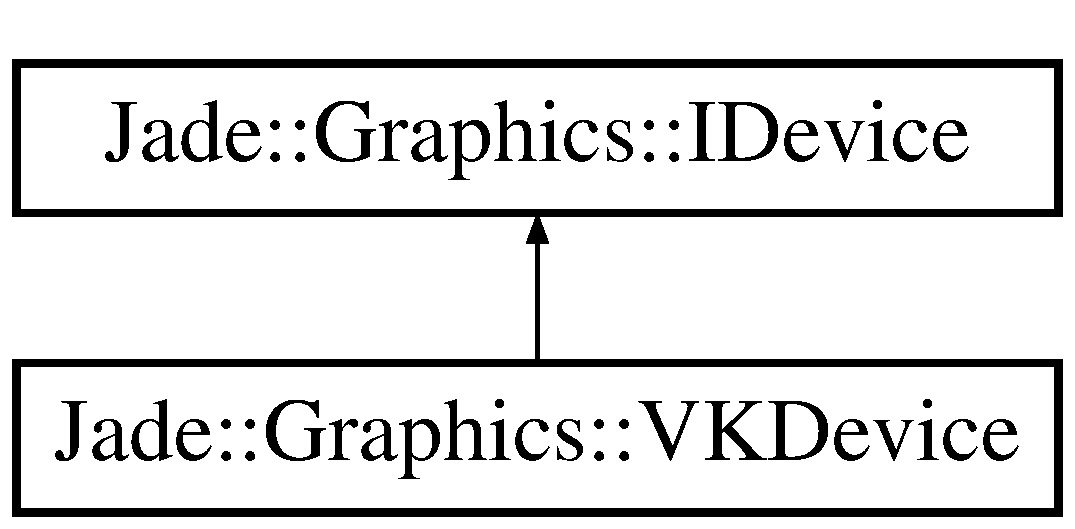
\includegraphics[height=2.000000cm]{class_jade_1_1_graphics_1_1_v_k_device}
\end{center}
\end{figure}
\subsection*{Public Member Functions}
\begin{DoxyCompactItemize}
\item 
\hypertarget{class_jade_1_1_graphics_1_1_v_k_device_ae8c46924cfda44f10d9c4d919492bf02}{}{\bfseries V\+K\+Device} (std\+::shared\+\_\+ptr$<$ \hyperlink{struct_jade_1_1_system_1_1_i_window}{System\+::\+I\+Window} $>$ window)\label{class_jade_1_1_graphics_1_1_v_k_device_ae8c46924cfda44f10d9c4d919492bf02}

\item 
\hypertarget{class_jade_1_1_graphics_1_1_v_k_device_aba3e595f7647339eb3bb0883a0b8754c}{}void {\bfseries Clear} (\hyperlink{struct_jade_1_1_math_1_1_color}{Math\+::\+Color} color) override\label{class_jade_1_1_graphics_1_1_v_k_device_aba3e595f7647339eb3bb0883a0b8754c}

\item 
\hypertarget{class_jade_1_1_graphics_1_1_v_k_device_a262ae03683d38b7f294e5750aa36a5df}{}void {\bfseries Present} () override\label{class_jade_1_1_graphics_1_1_v_k_device_a262ae03683d38b7f294e5750aa36a5df}

\end{DoxyCompactItemize}


The documentation for this class was generated from the following files\+:\begin{DoxyCompactItemize}
\item 
C\+:/\+Users/\+Ben/\+Documents/\+Git\+Hub/\+Jade/\+Jade/\+Source/\+Graphics/\+Device/V\+K\+Device.\+h\item 
C\+:/\+Users/\+Ben/\+Documents/\+Git\+Hub/\+Jade/\+Jade/\+Source/\+Graphics/\+Device/V\+K\+Device.\+cpp\end{DoxyCompactItemize}

\hypertarget{class_jade_1_1_graphics_1_1_widget}{}\section{Jade\+:\+:Graphics\+:\+:Widget Class Reference}
\label{class_jade_1_1_graphics_1_1_widget}\index{Jade\+::\+Graphics\+::\+Widget@{Jade\+::\+Graphics\+::\+Widget}}
Inheritance diagram for Jade\+:\+:Graphics\+:\+:Widget\+:\begin{figure}[H]
\begin{center}
\leavevmode
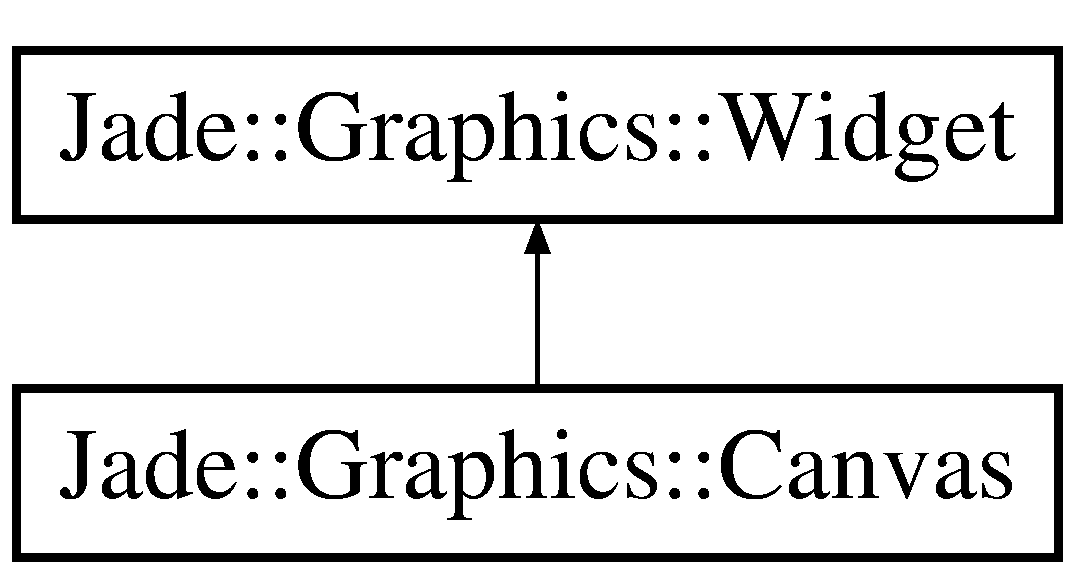
\includegraphics[height=2.000000cm]{class_jade_1_1_graphics_1_1_widget}
\end{center}
\end{figure}
\subsection*{Public Member Functions}
\begin{DoxyCompactItemize}
\item 
\hypertarget{class_jade_1_1_graphics_1_1_widget_a6b4cf0eb5064c61cf56ebb44681a2c60}{}virtual \hyperlink{class_jade_1_1_math_1_1_point}{Math\+::\+Point} {\bfseries Get\+Position} ()=0\label{class_jade_1_1_graphics_1_1_widget_a6b4cf0eb5064c61cf56ebb44681a2c60}

\item 
\hypertarget{class_jade_1_1_graphics_1_1_widget_ab89794b5d4ee480828ea6de52c9b1048}{}virtual void {\bfseries Set\+Position} (int x, int y)=0\label{class_jade_1_1_graphics_1_1_widget_ab89794b5d4ee480828ea6de52c9b1048}

\item 
\hypertarget{class_jade_1_1_graphics_1_1_widget_a16d7008052de562ea8d52b3c97c801c3}{}virtual void {\bfseries Show} ()=0\label{class_jade_1_1_graphics_1_1_widget_a16d7008052de562ea8d52b3c97c801c3}

\item 
\hypertarget{class_jade_1_1_graphics_1_1_widget_a0ad3acf723f554f315da105d9b36e921}{}virtual void {\bfseries Hide} ()=0\label{class_jade_1_1_graphics_1_1_widget_a0ad3acf723f554f315da105d9b36e921}

\item 
\hypertarget{class_jade_1_1_graphics_1_1_widget_adb8d9882202a73428260cbd3d8b15f9a}{}virtual void \hyperlink{class_jade_1_1_graphics_1_1_widget_adb8d9882202a73428260cbd3d8b15f9a}{Draw} ()=0\label{class_jade_1_1_graphics_1_1_widget_adb8d9882202a73428260cbd3d8b15f9a}

\begin{DoxyCompactList}\small\item\em Submits the widget information to the current device for rendering. \end{DoxyCompactList}\end{DoxyCompactItemize}


The documentation for this class was generated from the following file\+:\begin{DoxyCompactItemize}
\item 
C\+:/\+Users/\+Ben/\+Documents/\+Git\+Hub/\+Jade/\+Jade/\+Source/\+Graphics/\+Widget/Widget.\+h\end{DoxyCompactItemize}

\hypertarget{class_jade_1_1_system_1_1_window}{}\section{Jade\+:\+:System\+:\+:Window Class Reference}
\label{class_jade_1_1_system_1_1_window}\index{Jade\+::\+System\+::\+Window@{Jade\+::\+System\+::\+Window}}
\subsection*{Public Member Functions}
\begin{DoxyCompactItemize}
\item 
\hypertarget{class_jade_1_1_system_1_1_window_a3d6db589237ba8c173e876b4da44261f}{}bool {\bfseries Is\+Open} () const \label{class_jade_1_1_system_1_1_window_a3d6db589237ba8c173e876b4da44261f}

\item 
\hypertarget{class_jade_1_1_system_1_1_window_a28c7ebb91e752ec16f1550393f8d96b5}{}int {\bfseries Get\+Width} () const \label{class_jade_1_1_system_1_1_window_a28c7ebb91e752ec16f1550393f8d96b5}

\item 
\hypertarget{class_jade_1_1_system_1_1_window_adfc7b77a2b4f48d08da1e1e41543b44a}{}void {\bfseries Set\+Width} (int width) const \label{class_jade_1_1_system_1_1_window_adfc7b77a2b4f48d08da1e1e41543b44a}

\item 
\hypertarget{class_jade_1_1_system_1_1_window_a73e056060c2af44d3f8fd0f950fe3192}{}int {\bfseries Get\+Height} () const \label{class_jade_1_1_system_1_1_window_a73e056060c2af44d3f8fd0f950fe3192}

\item 
\hypertarget{class_jade_1_1_system_1_1_window_a15efc837b2906cbd8b521bbe355fd80c}{}void {\bfseries Set\+Height} (int height) const \label{class_jade_1_1_system_1_1_window_a15efc837b2906cbd8b521bbe355fd80c}

\item 
\hypertarget{class_jade_1_1_system_1_1_window_a3b9474c8b49b42b3d5657dc2c21fd59c}{}float {\bfseries Get\+Aspect\+Ratio} () const \label{class_jade_1_1_system_1_1_window_a3b9474c8b49b42b3d5657dc2c21fd59c}

\item 
\hypertarget{class_jade_1_1_system_1_1_window_a1489a0e9995db4c89b5be8a8ab02971b}{}void $\ast$ {\bfseries Handle} () const \label{class_jade_1_1_system_1_1_window_a1489a0e9995db4c89b5be8a8ab02971b}

\item 
\hypertarget{class_jade_1_1_system_1_1_window_a61e1612462c18be13dc3b2e1a01dfce5}{}std\+::string {\bfseries Get\+Title} () const \label{class_jade_1_1_system_1_1_window_a61e1612462c18be13dc3b2e1a01dfce5}

\item 
\hypertarget{class_jade_1_1_system_1_1_window_a275f84ab49b78f1ba46612447f5683e1}{}void {\bfseries Set\+Title} (std\+::string title) const \label{class_jade_1_1_system_1_1_window_a275f84ab49b78f1ba46612447f5683e1}

\item 
\hypertarget{class_jade_1_1_system_1_1_window_a0d6abe35b92fd2d2598919062b0e6b0c}{}void {\bfseries Set\+Icon} (std\+::string filename) const \label{class_jade_1_1_system_1_1_window_a0d6abe35b92fd2d2598919062b0e6b0c}

\item 
\hypertarget{class_jade_1_1_system_1_1_window_ae36b19e7f8e05bb0e1af58063e1f3f7b}{}bool {\bfseries Is\+Fullscreen} () const \label{class_jade_1_1_system_1_1_window_ae36b19e7f8e05bb0e1af58063e1f3f7b}

\item 
\hypertarget{class_jade_1_1_system_1_1_window_a1b05887e9ddd213ba43a16a4caf5d85f}{}bool {\bfseries Is\+Active} () const \label{class_jade_1_1_system_1_1_window_a1b05887e9ddd213ba43a16a4caf5d85f}

\item 
\hypertarget{class_jade_1_1_system_1_1_window_a092090dd6658c8edca8c9030d0c00490}{}std\+::shared\+\_\+ptr$<$ \hyperlink{struct_jade_1_1_system_1_1_i_window}{I\+Window} $>$ {\bfseries Get\+I\+Window} () const \label{class_jade_1_1_system_1_1_window_a092090dd6658c8edca8c9030d0c00490}

\item 
\hypertarget{class_jade_1_1_system_1_1_window_aff8a9ea34e259660afda6d1f3696434a}{}\hyperlink{class_jade_1_1_system_1_1_timer}{Timer} {\bfseries Get\+Time} () const \label{class_jade_1_1_system_1_1_window_aff8a9ea34e259660afda6d1f3696434a}

\item 
\hypertarget{class_jade_1_1_system_1_1_window_a9679baac6ae29568307624fb2dfcef3f}{}\hyperlink{struct_jade_1_1_input_1_1_input}{Input\+::\+Input} {\bfseries Get\+Input} () const \label{class_jade_1_1_system_1_1_window_a9679baac6ae29568307624fb2dfcef3f}

\item 
\hypertarget{class_jade_1_1_system_1_1_window_a7c43d89407ac25953bc0f73d34fffe33}{}{\bfseries Window} (int width, int height, int x, int y, std\+::string title, bool fullscreen)\label{class_jade_1_1_system_1_1_window_a7c43d89407ac25953bc0f73d34fffe33}

\item 
\hypertarget{class_jade_1_1_system_1_1_window_a06eb435ef0e8dfed2b970e28363de3d7}{}bool {\bfseries Poll\+Events} () const \label{class_jade_1_1_system_1_1_window_a06eb435ef0e8dfed2b970e28363de3d7}

\item 
\hypertarget{class_jade_1_1_system_1_1_window_ac450a8a630467335661f4fd16a7f660e}{}void {\bfseries Close} () const \label{class_jade_1_1_system_1_1_window_ac450a8a630467335661f4fd16a7f660e}

\end{DoxyCompactItemize}


The documentation for this class was generated from the following file\+:\begin{DoxyCompactItemize}
\item 
C\+:/\+Users/\+Ben/\+Documents/\+Git\+Hub/\+Jade/\+Jade/\+Source/\+System/\+Window/Window.\+h\end{DoxyCompactItemize}

%--- End generated contents ---

% Index
\backmatter
\newpage
\phantomsection
\clearemptydoublepage
\addcontentsline{toc}{chapter}{Index}
\printindex

\end{document}
